\section{The Aeroacoustic Source Field}
\label{sect:source}
%Ribner presented an alternative approach to Lighthill's acoustic analogy which posited fluctuating fluid dilatations as the source of aeroacoustic emission \citep{Ribner1962}.
%This is a reinterpretation of Lighthill's source, which in subsonic, unheated, turbulent jets consists of fluctuating momentum flux.
%The driving factor behind Ribner's analysis is the conceptual simplification of the aeroacoustic sources: Lighthill's quadrupoles are replaced by the contraction or expansion of fluid elements (confusingly identified alternatively as \emph{pseudosound} or \emph{pseudo-pressure}) due to the fluctuating momentum flux, which in turn drive the acoustic field.
%This conceptual simplicity makes the dilatation-based approach to the acoustic analogy particularly attractive to the experimentalist for high-speed (though subsonic), turbulent flows.
%The analysis, described briefly in the subsequent section, is (relatively) simple to perform computationally, relying exclusively on second-order derivatives (unlike the third-order differential equation derived by Lilley \citep{Lilley2003}) which include a natural filtering mechanism.
%More importantly, the pseudosound field (which is the direct precursor to the source field) can be directly compared against the time-resolved hydrodynamic pressure field measured in the irrotational near-field, thus serving as a helpful validation of the computations.
%
%\section{Ribner's Acoustic Analogy}
%To briefly acquaint the reader, an overview of Ribner's analysis will be provided here.
%Further details can be found in Ribner \citep{Ribner1962} if the reader is so inclined. 
%Ribner's analysis directly follows from Lighthill's, and as such includes the same restrictions on the applicable class of flows.
%Starting from Lighthill's analogy (\eq{eq:lighthill_analogy}), the source term is first reduced by neglecting viscosity and entropic fluctuations (thereby assuming that the flow is of high Reynolds number and unheated), leaving only the Reynolds stress terms:
%\begin{equation}
%	\frac{1}{c^2}\frac{\partial^2 p}{\partial t^2} - \nabla^2 p = \nabla \cdot \nabla \cdot \rho \mathbf{u} \otimes \mathbf{u}.
%\end{equation}
%Ribner then split the pressure fluctuations into an acoustic component and an incompressible component (pseudosound, which is associated with the convective hydrodynamic fluctuations), $p' + p_0 = p_a + p_s$. 
%The incompressible component of the flow will then satisfy
%\begin{equation}
%	 \rho \frac{\partial}{\partial t} (\nabla \cdot \mathbf{v} )  = 0
%\end{equation}
%where $\mathbf{v}$ is now used in place of $\mathbf{u}$ to signify an incompressible (solenoidal) velocity field. 
%Therefore, 
%\begin{equation}
%	- \nabla^2 p_s = \nabla \cdot \nabla \cdot \rho_0 \mathbf{v} \otimes \mathbf{v}.
%	\label{eq:solenoidal_pressure}
%\end{equation}
%Ribner's analysis then assumes that the full density and velocity fields can be approximated as the incompressible (solenoidal) fields (the higher-order terms scaling with the \textit{fluctuating} Mach number \citep{Ristorcelli1997}), thus producing Ribner's Dilatation Equation
%\begin{equation}
%	\frac{1}{c^2}\frac{\partial^2 p_a}{\partial t^2} - \nabla^2 p_a = -\frac{1}{c^2}\frac{\partial^2 p_s}{\partial t^2}.
%	\label{eq:ribner_source}
%\end{equation} 
%
%In this way, acoustic pressure field is ultimately linked to the time rate of change of the dilatation (see Ristorcelli \citep{Ristorcelli1997} for a very enlightening perturbation analysis which makes this relationship far more clear).
%This is far from a controversial assertion; numerous other researchers have used the dilatation field to examine the aeroacoustic phenomena (primarily using DNS or LES simulations); see Mitchell \etal \citep{Mitchell1995}, Colonius \etal \citep{Colonius1997}, or Freund \etal \citep{Freund2000} for examples.
%In fact, this relationship can easily be illustrated, as has been done in \fig{fig:LES_dilatation}. 
%Here, phase-averaged data at two phases has been plotted from a simulated Mach 1.3 jet excited by plasma actuators at $St_{DF} = 0.25$; details of the numerical methods and results can be found in Speth \& Gaitonde \citep{Speth2014}. 
%The toroidal structures generated by the excitation have been visualized in the foreground using Q-criterion, and the dilatation field in the background in grayscale.
%Highly coherent dilatation waves can be observed convecting alongside the large-scale structures near the shear layer. 
%Further out radially, the dilatation field becomes less coherent and more indicative of far-field propagating pressure waves.
%Broadly and qualitatively speaking, the connection between the large-scale structures and the acoustic emission is clear; the current work attempts to evaluate this relationship more formally.
%\begin{figure}
%	\centering
%	\begin{subfigure}{.5\textwidth}
%		\centering
%		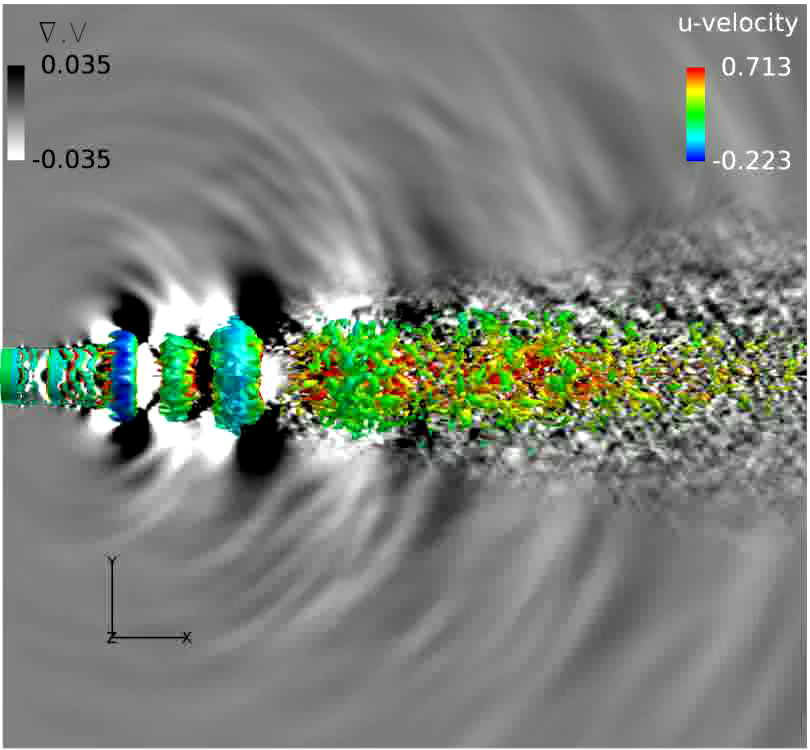
\includegraphics[width=0.95\linewidth]{Figures/LES_dilatation1.jpg}
%		\caption{}
%	\end{subfigure}%
%	\begin{subfigure}{.5\textwidth}
%		\centering
%		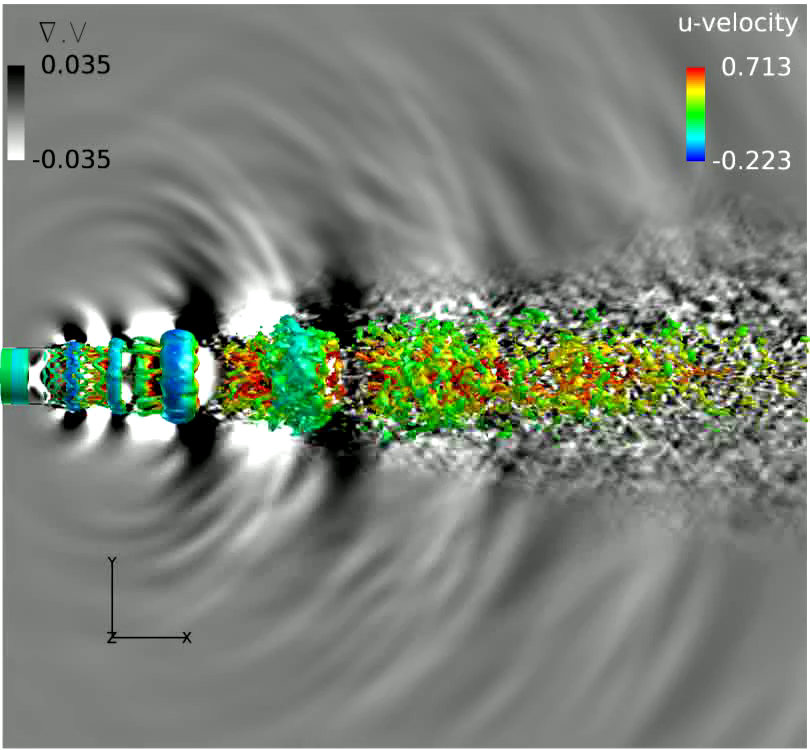
\includegraphics[width=0.95\linewidth]{Figures/LES_dilatation2.jpg}
%		\caption{}
%	\end{subfigure}
%	\caption{Two phases of actuation taken from the implicit LES database of Speth \& Gaitonde \citep{Speth2014}. Isosurfaces are computed from Q-criterion and colored by axial velocity, and the background corresponds to dilatation.}
%	\label{fig:LES_dilatation}
%\end{figure}
%\section{Numerical Methodology}
%Computing the aeroacoustic source per Ribner's dilatation method from the estimated, time-resolved velocity field constitutes a three-step process. 
%First, the solenoidal velocity field is computed via the Helmholtz' decomposition; the double divergence of the resulting stress tensor is then used as the source of Poisson's equation to calculate the pseudo-pressure field. 
%Finally, the pseudo-pressure field is filtered in time using an energy threshold in the wavelet domain, and the second time derivative of the resultant field is computed, producing the source field.
%This process is outlined in the following sections.
%\subsubsection{Helmholtz Decomposition}
%For a given vector field, $\mathbf{F}$, Helmholtz's theorem states that any sufficiently smooth vector field can be linearly decomposed into irrotational and solenoidal vector fields, as
%\begin{equation}
%\mathbf{F} = \mathbf{F}_{potential} + \mathbf{F}_{rotational} = \nabla \Phi + \nabla \times \Psi
%\end{equation}
%where $\Phi$ is a scalar field and $\Psi$ is a vector field.
%From basic vector calculus properties, one can therefore compute these solenoidal and irrotational components by taking the divergence of this equation, leading to:
%\begin{equation}
%\nabla \cdot \mathbf{F} = \nabla^{2} \Phi
%\end{equation}
%which is simply Poisson's equation, where in the context of a velocity decomposition the forcing term is simply the divergence of the flow field (that is, the dilatation).
%
%This initially presents a quandary for the researcher, as only planar PIV measurements are available, and hence the azimuthal velocity and derivative terms are unknown.
%As mentioned previously, the flow-field in a natural, high Reynolds number jet is a combination of numerous azimuthal Fourier modes.
%Though the velocity field has been found to contain a significant amount of energy at the higher order modes, the axisymmetric mode is still the dominant mode within the potential core region of the jet \citep{Glauser1987}.
%Additionally, it is the acoustic emission from the coherent large-scale toroidal structure generated by excitation that is the primary focus of this endeavor, not the full acoustic emission from the relatively incoherent natural turbulence.
%Due to the specific nature of the excitation (axisymmetric excitation), the azimuthal components of the flow are not expected to be significant.
%
%The database of Speth \& Gaitonde \citep{Speth2014} was provided to the author for the purpose of validating this assumption.
%Comparisons between the near-field pressure response to excitation of the experimental (\sect{sect:nearfield}) and numerical databases were performed in the reference, and a good match was found.
%Sample results for the pressure and radial velocity field for a single azimuthal plane are shown in \fig{fig:LES_streamwise_phavg}; these results correspond to an actuation phase of $1.4 \pi$ for $St_{DF} = 0.05$, and have been phase-averaged over nine actuation cycles.
%(While less than desirable, the computationalists could not store the full, instantaneous 3-D velocity fields due to harddrive limitations. The $St_{DF} = 0.05$ was therefore chosen for this analysis since it contained the fewest number of actuation cycles and thus has the highest level of incoherent fluctuations.)
%From these plots, a large-scale coherent structure generated by the excitation can easily be identified, centered at $x/D = 2.1, r/D = 0.5$.
%\begin{figure}
%	\centering
%	\begin{subfigure}{0.75\textwidth}
%		\centering
%		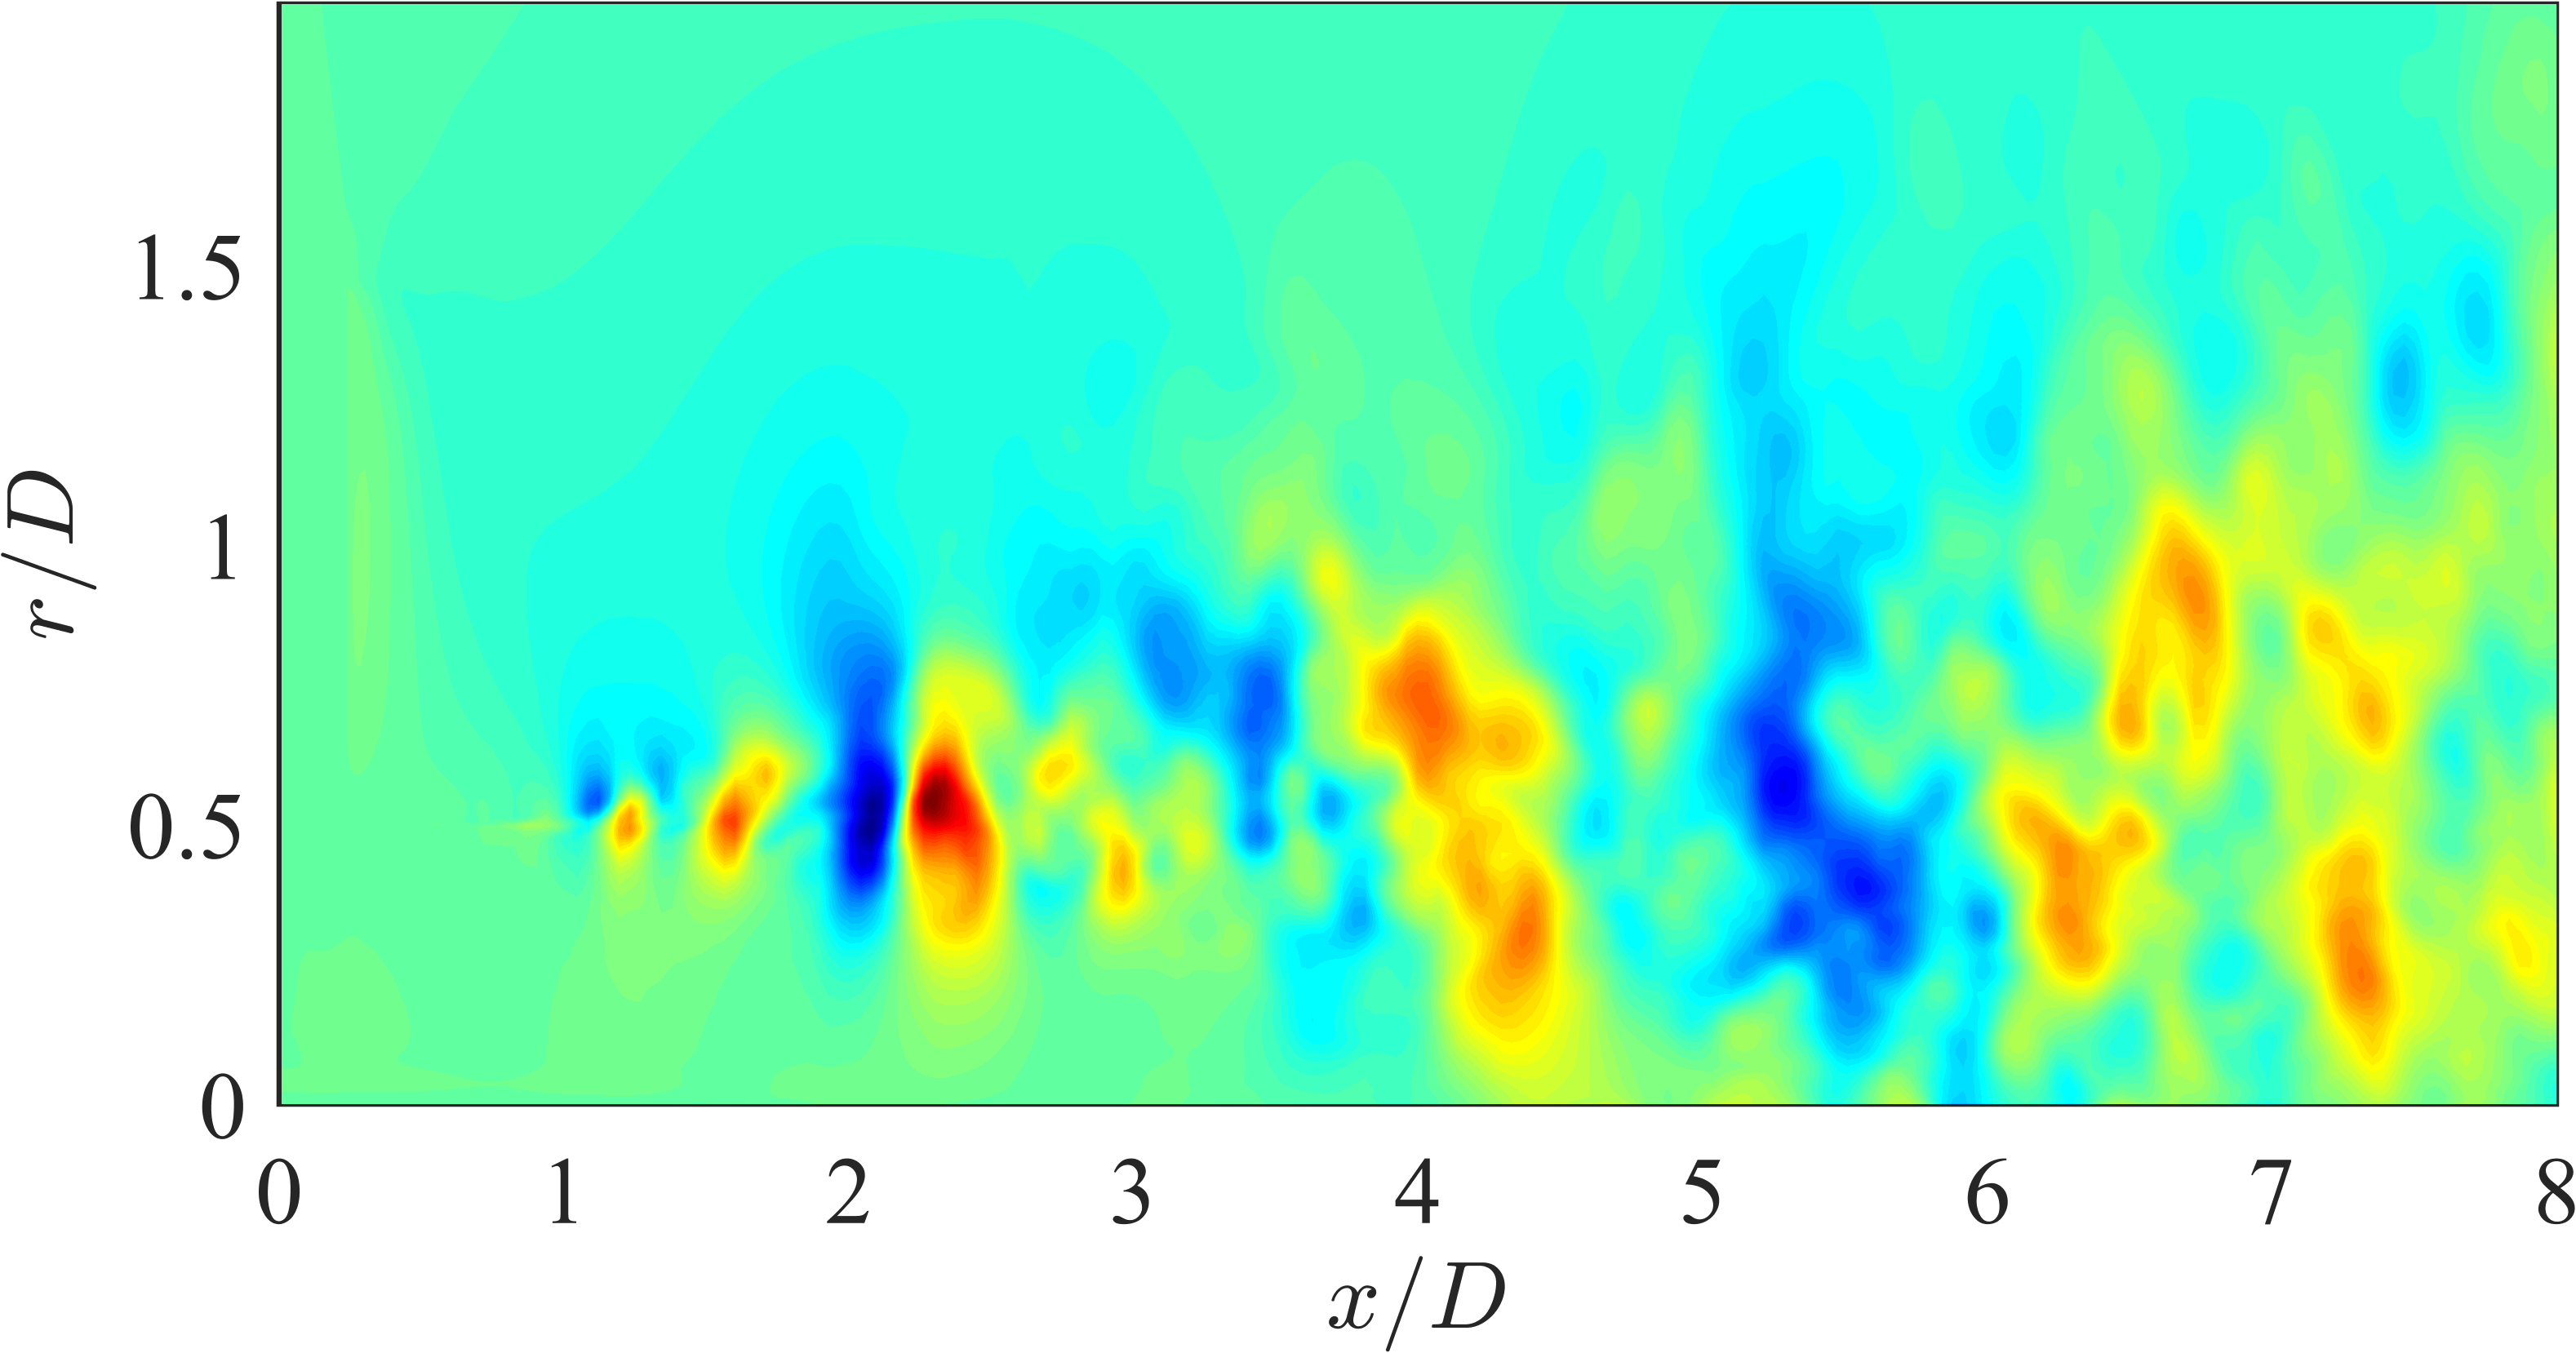
\includegraphics[width=0.95\linewidth]{Figures/LES_phavg_streamwise_Ur.png}
%		\caption{}
%	\end{subfigure}\\
%	\begin{subfigure}{0.75\textwidth}
%		\centering
%		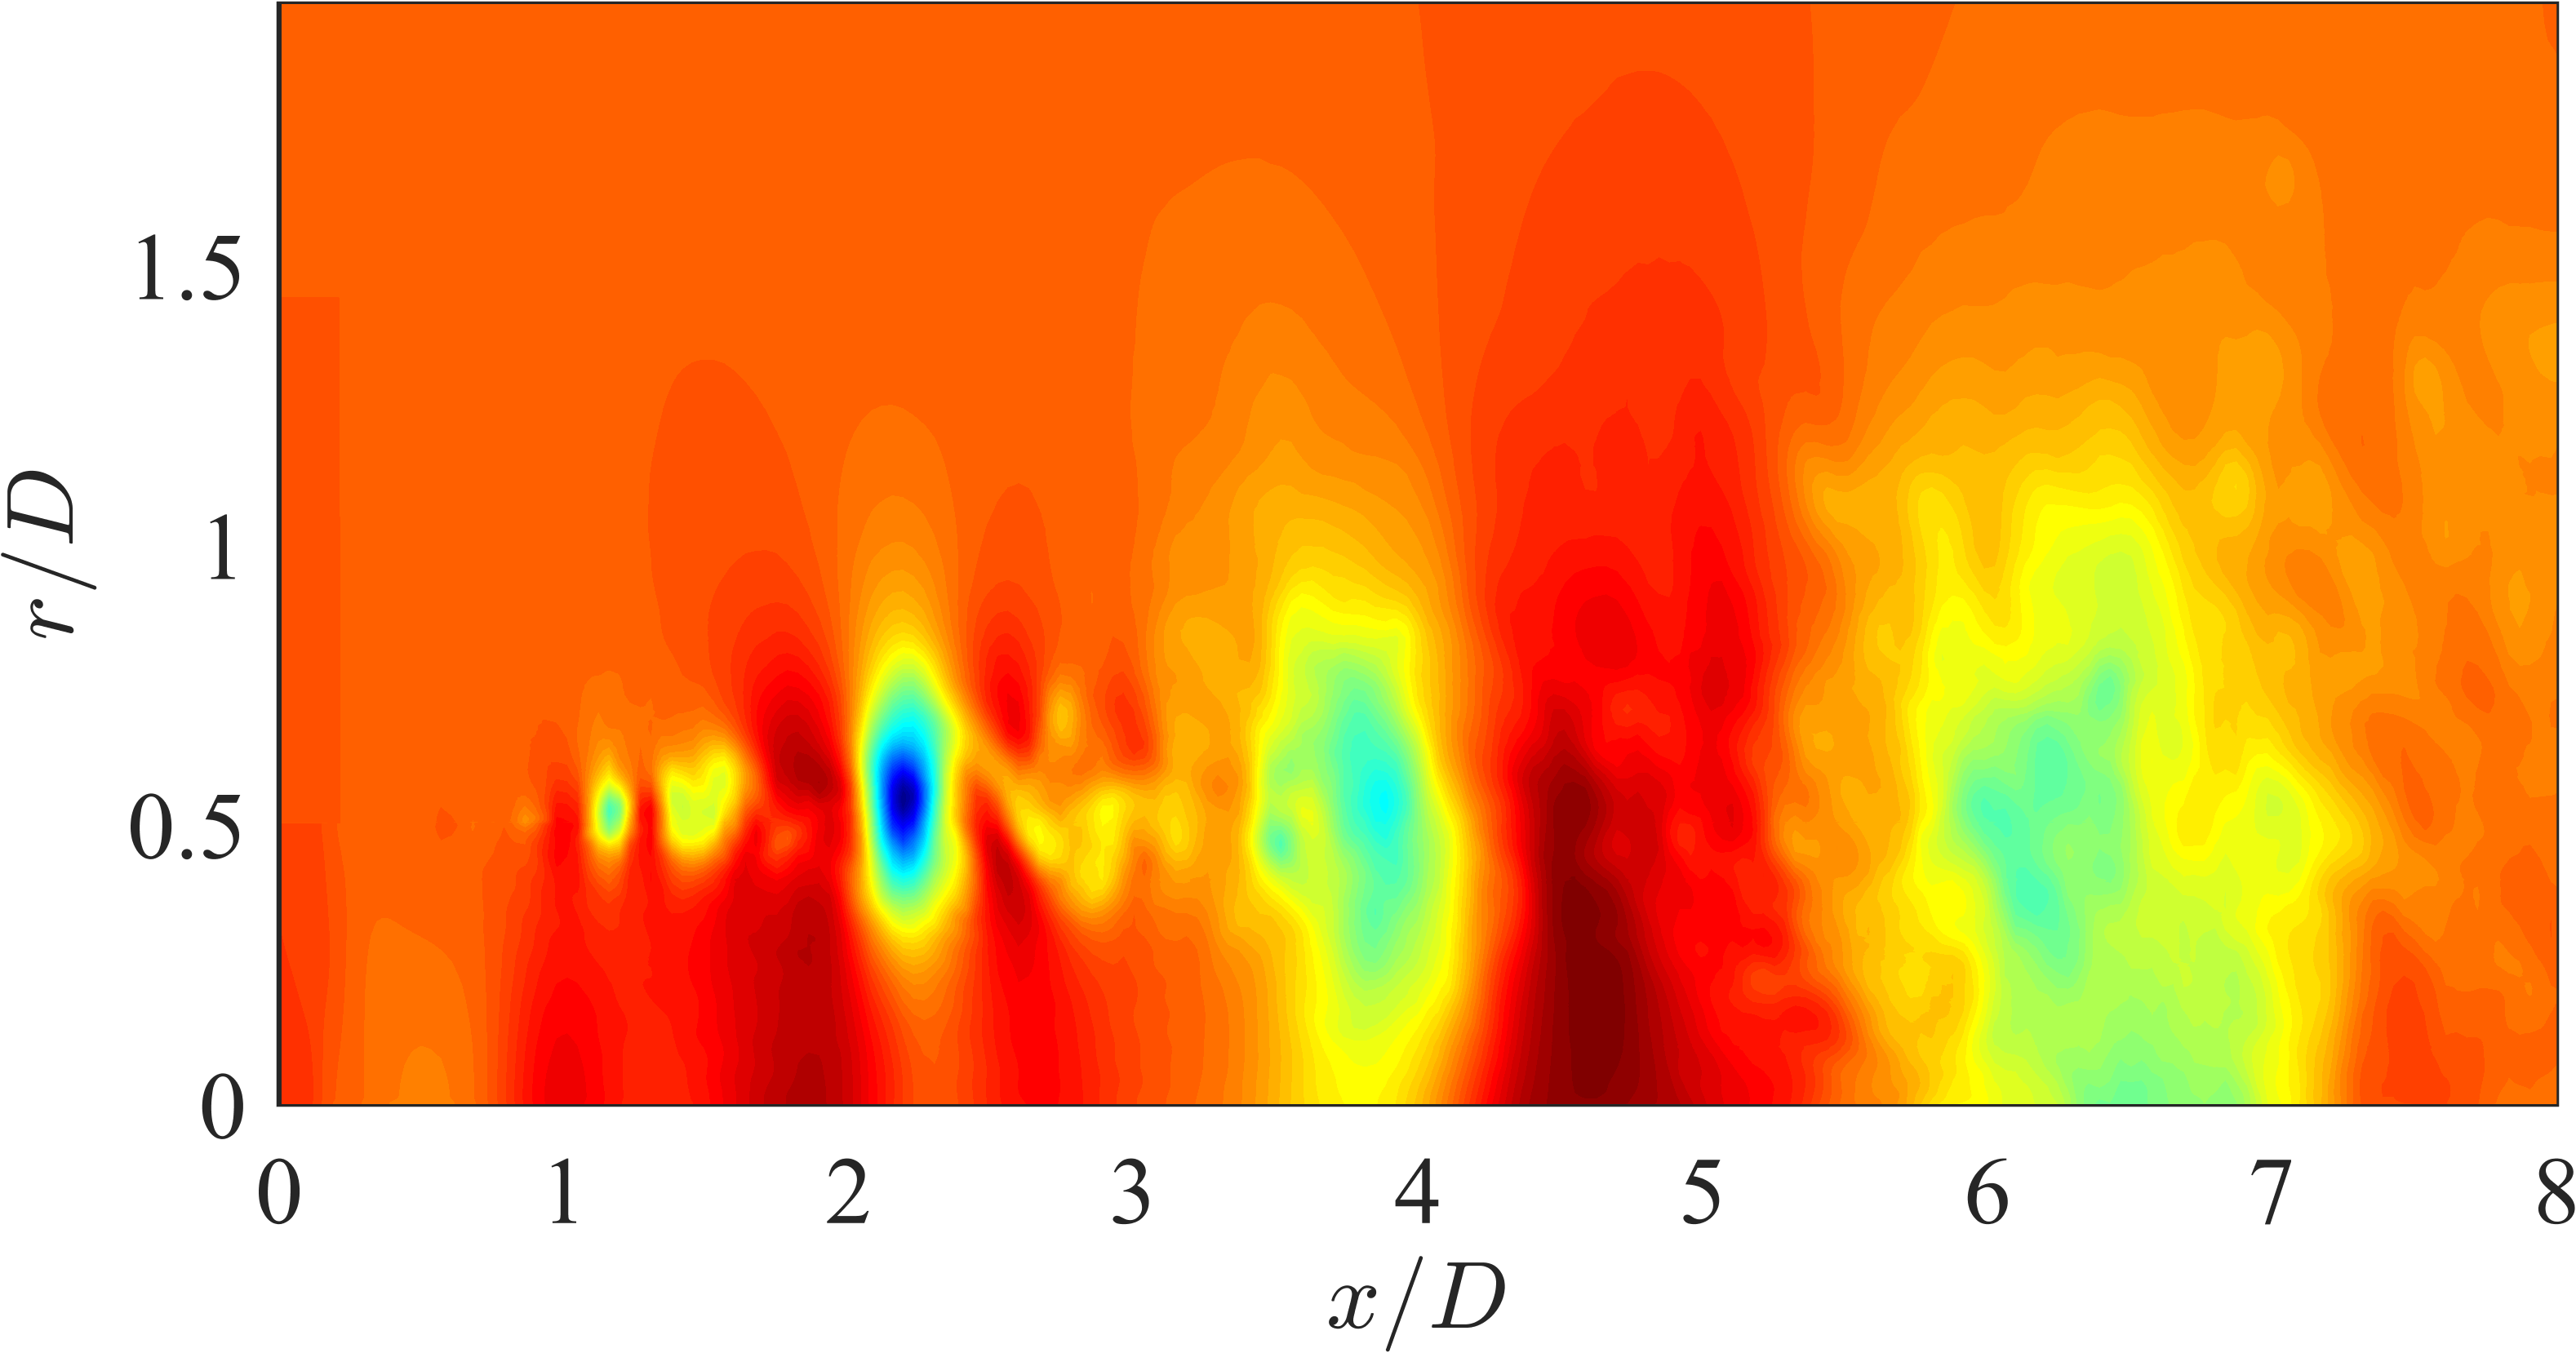
\includegraphics[width=0.95\linewidth]{Figures/LES_phavg_streamwise_p.png}
%		\caption{}
%	\end{subfigure}
%	\caption{Axial velocity (a) and pressure (b) contours taken from the database of Speth \& Gaitonde \citep{Speth2014} for $St_{DF} = 0.05$.}
%	\label{fig:LES_streamwise_phavg}
%\end{figure}
%
%The azimuthal velocity field corresponding to the axial location of the large-scale structure is shown in \fig{fig:LES_cross_phavg}.
%While the azimuthal velocity is, unsurprisingly, non-zero, the field is highly incoherent as compared to the radial or axial velocity fields and of much lower amplitude.
%Finally, The dilatation field computed using the full 3-D gradients and the partial dilatation field computed using only the radial and axial gradients can be found in \fig{fig:LES_streamwise_dil}.
%Because there are weak azimuthal structures inherent even in the excited turbulent jet, a noticeable difference between the two- and full three-component dilatation fields is readily apparent in terms of fluctuation amplitude.
%However, the spatial structure of the full dilatation field is largely retained in the reduced (two-component) dilatation field, just at an amplitude reduced by a nearly constant factor of $\sim 2$.
%Because of this, the loss of the azimuthal gradient information is not expected to be produce unacceptable errors in the final solution.
%Therefore, the azimuthal terms are dropped, leaving
%\begin{equation}
%\frac{\partial U_r}{\partial r} + \frac{\partial U_x}{\partial x} + \frac{U_r}{r} = \frac{1}{r} \frac{\partial \Phi}{\partial r} + \frac{\partial^2 \Phi}{\partial r^2} + \frac{\partial^2 \Phi}{\partial x^2}.
%\label{eq:helmholtz}
%\end{equation}
%\begin{figure}
%	\centering
%	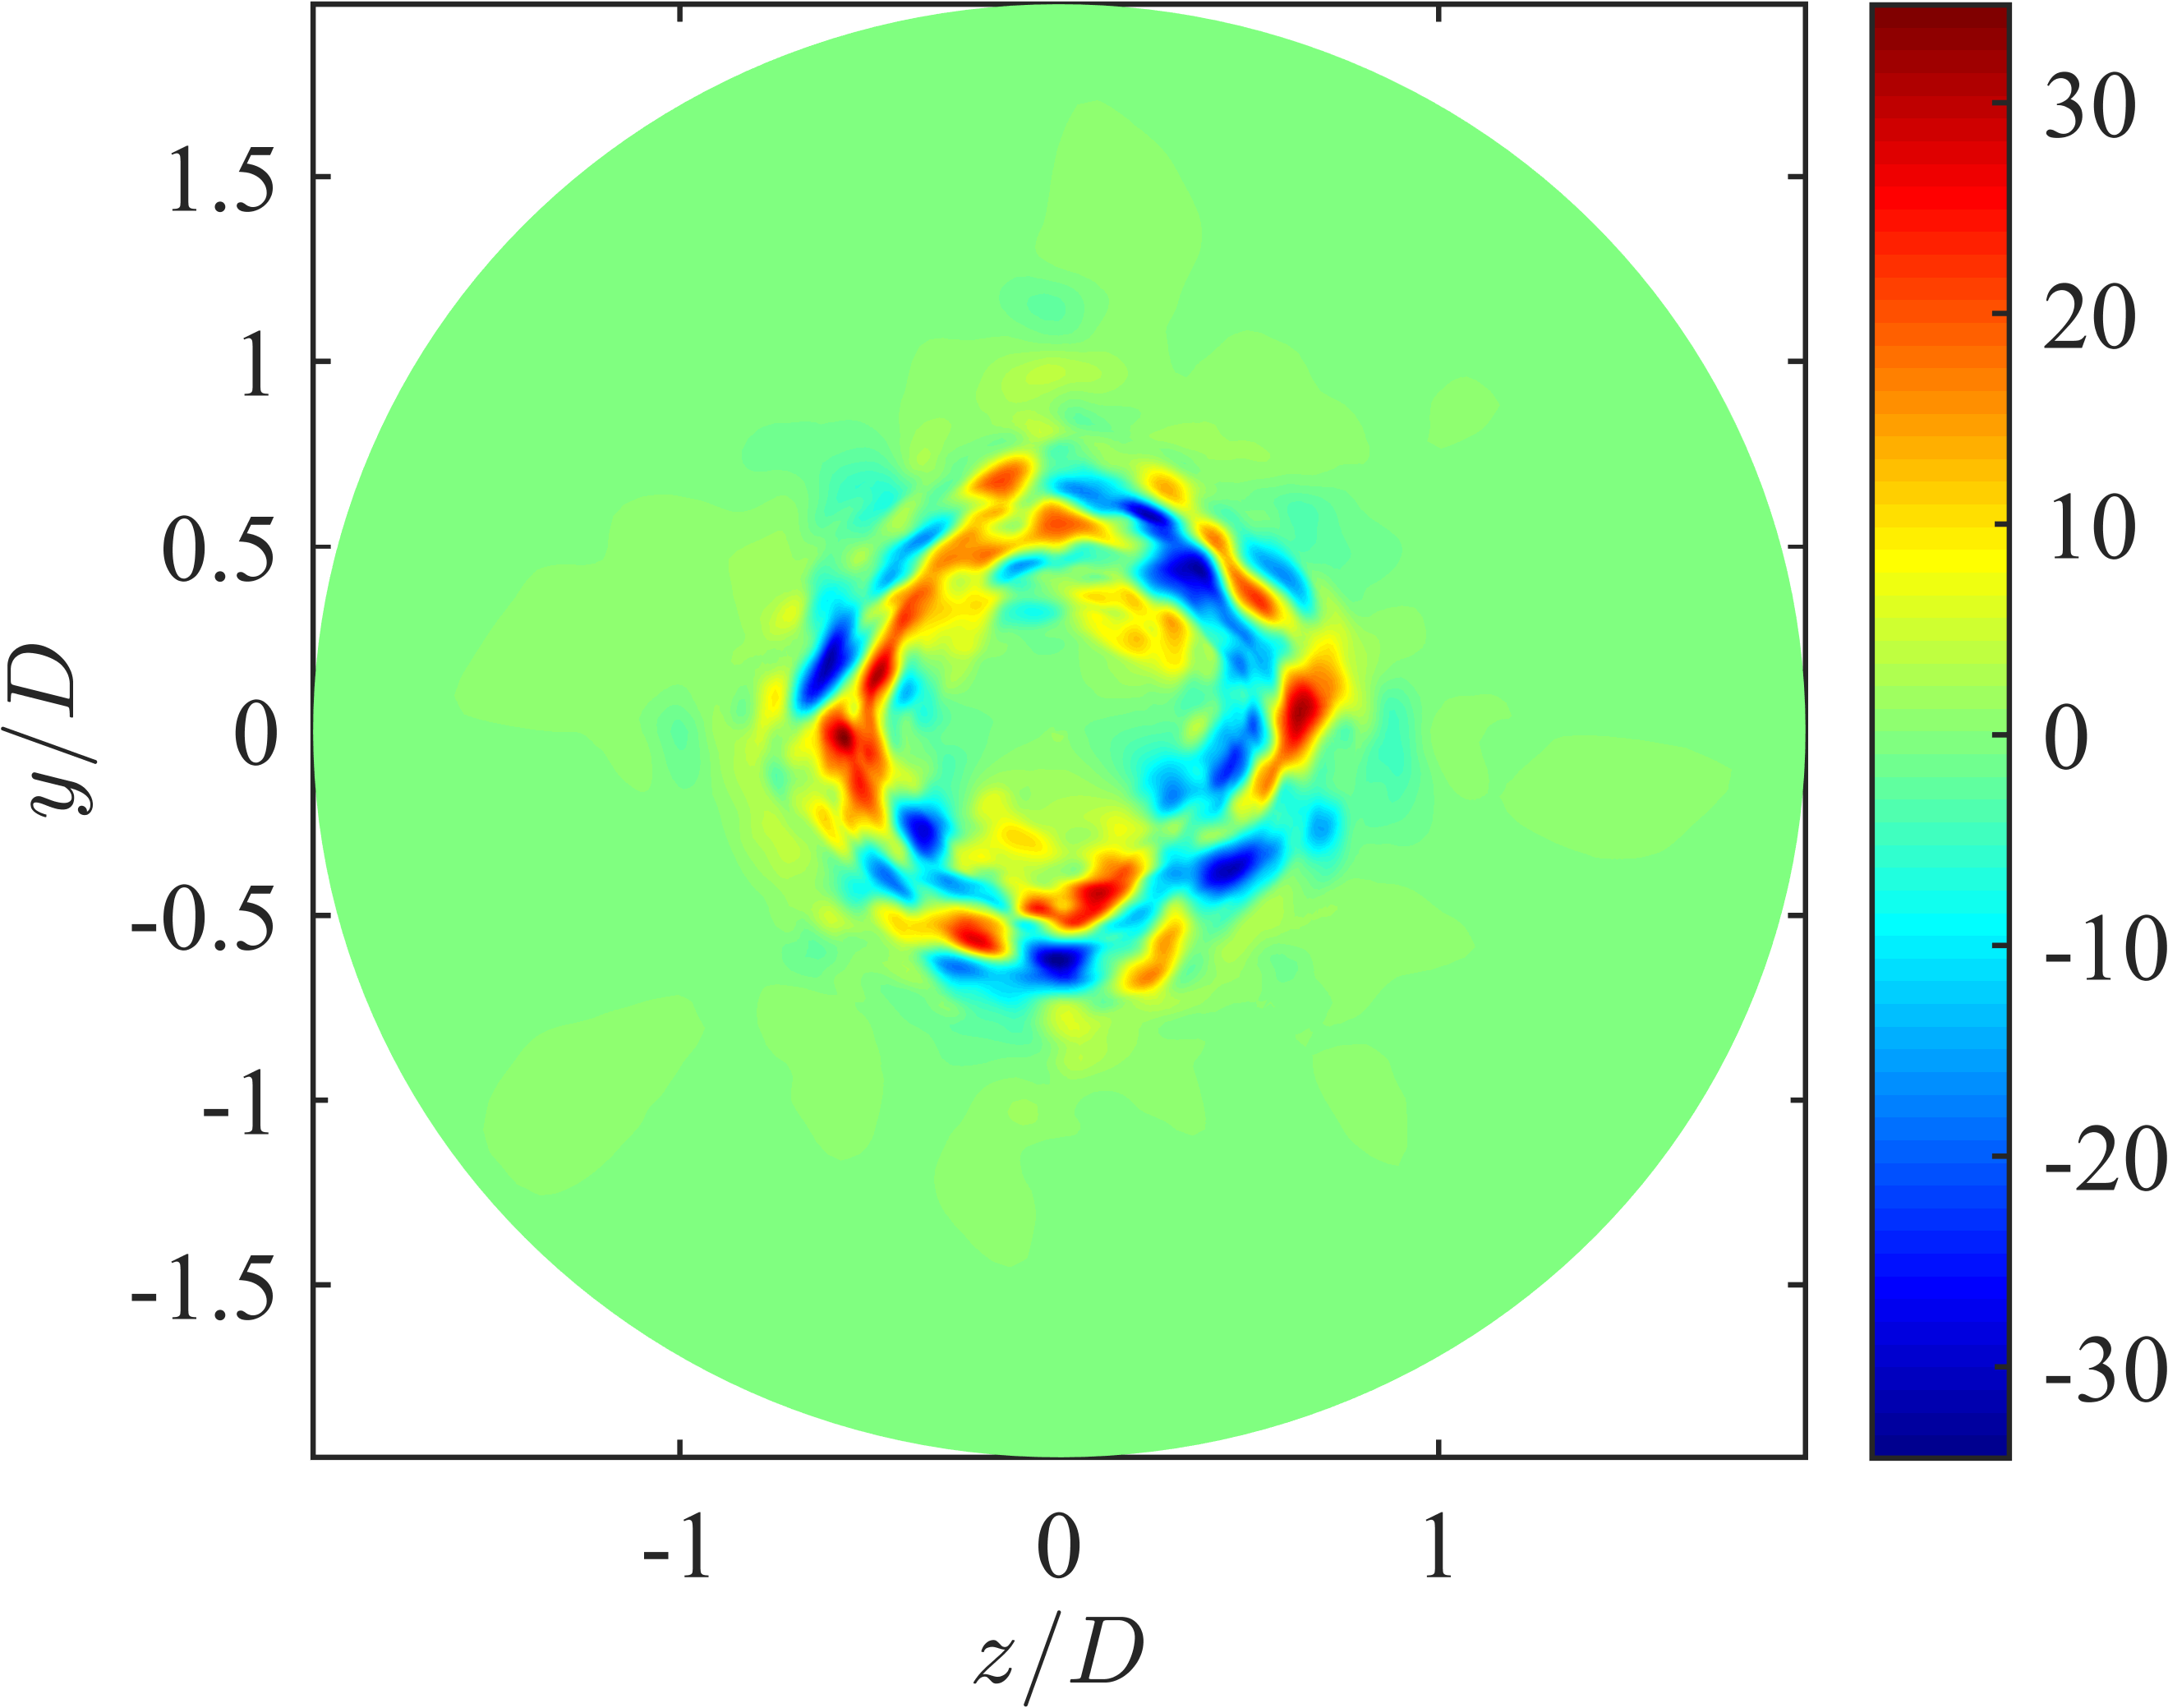
\includegraphics[width = 3.5in]{Figures/LES_phavg_cross_velocity.png}
%	\caption{Azimuthal velocity at $x/D = 2.1$ for the same instance as the previous figure; units are in m/s.}
%	\label{fig:LES_cross_phavg}
%\end{figure}
%\begin{figure}
%	\centering
%	\begin{subfigure}{0.75\textwidth}
%		\centering
%		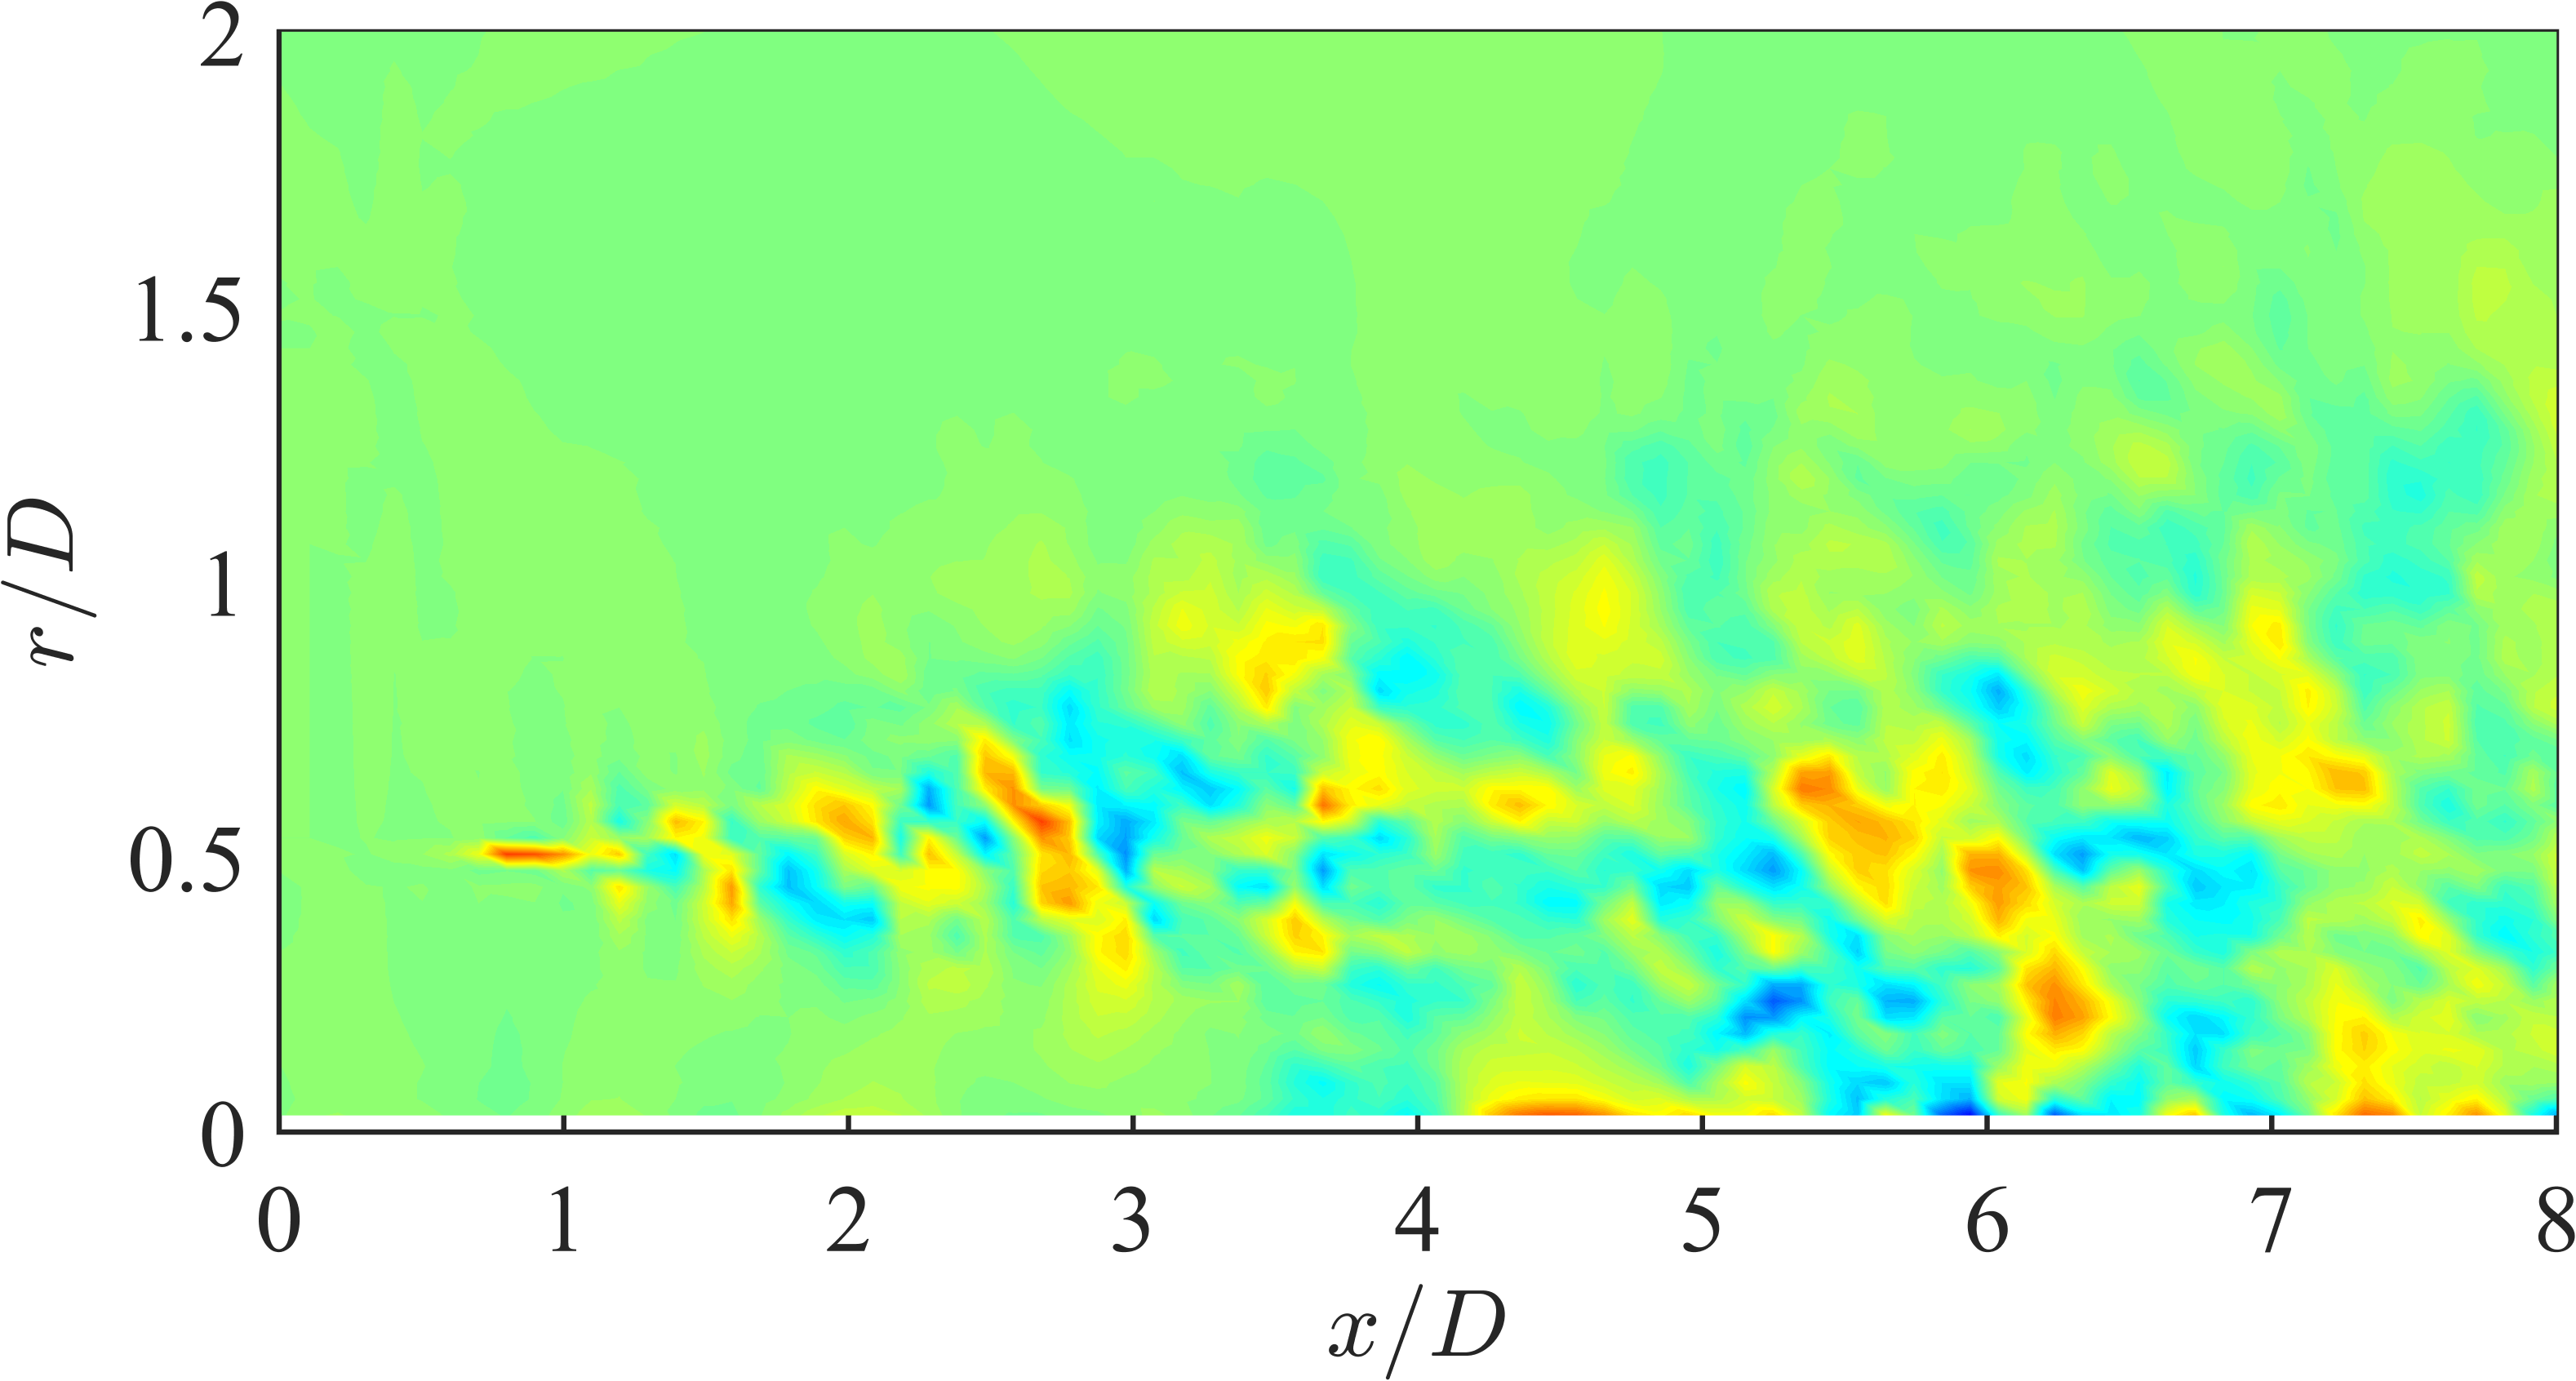
\includegraphics[width=0.95\linewidth]{Figures/LES_2CDil.png}
%		\caption{}
%	\end{subfigure}\\
%	\begin{subfigure}{0.75\textwidth}
%		\centering
%		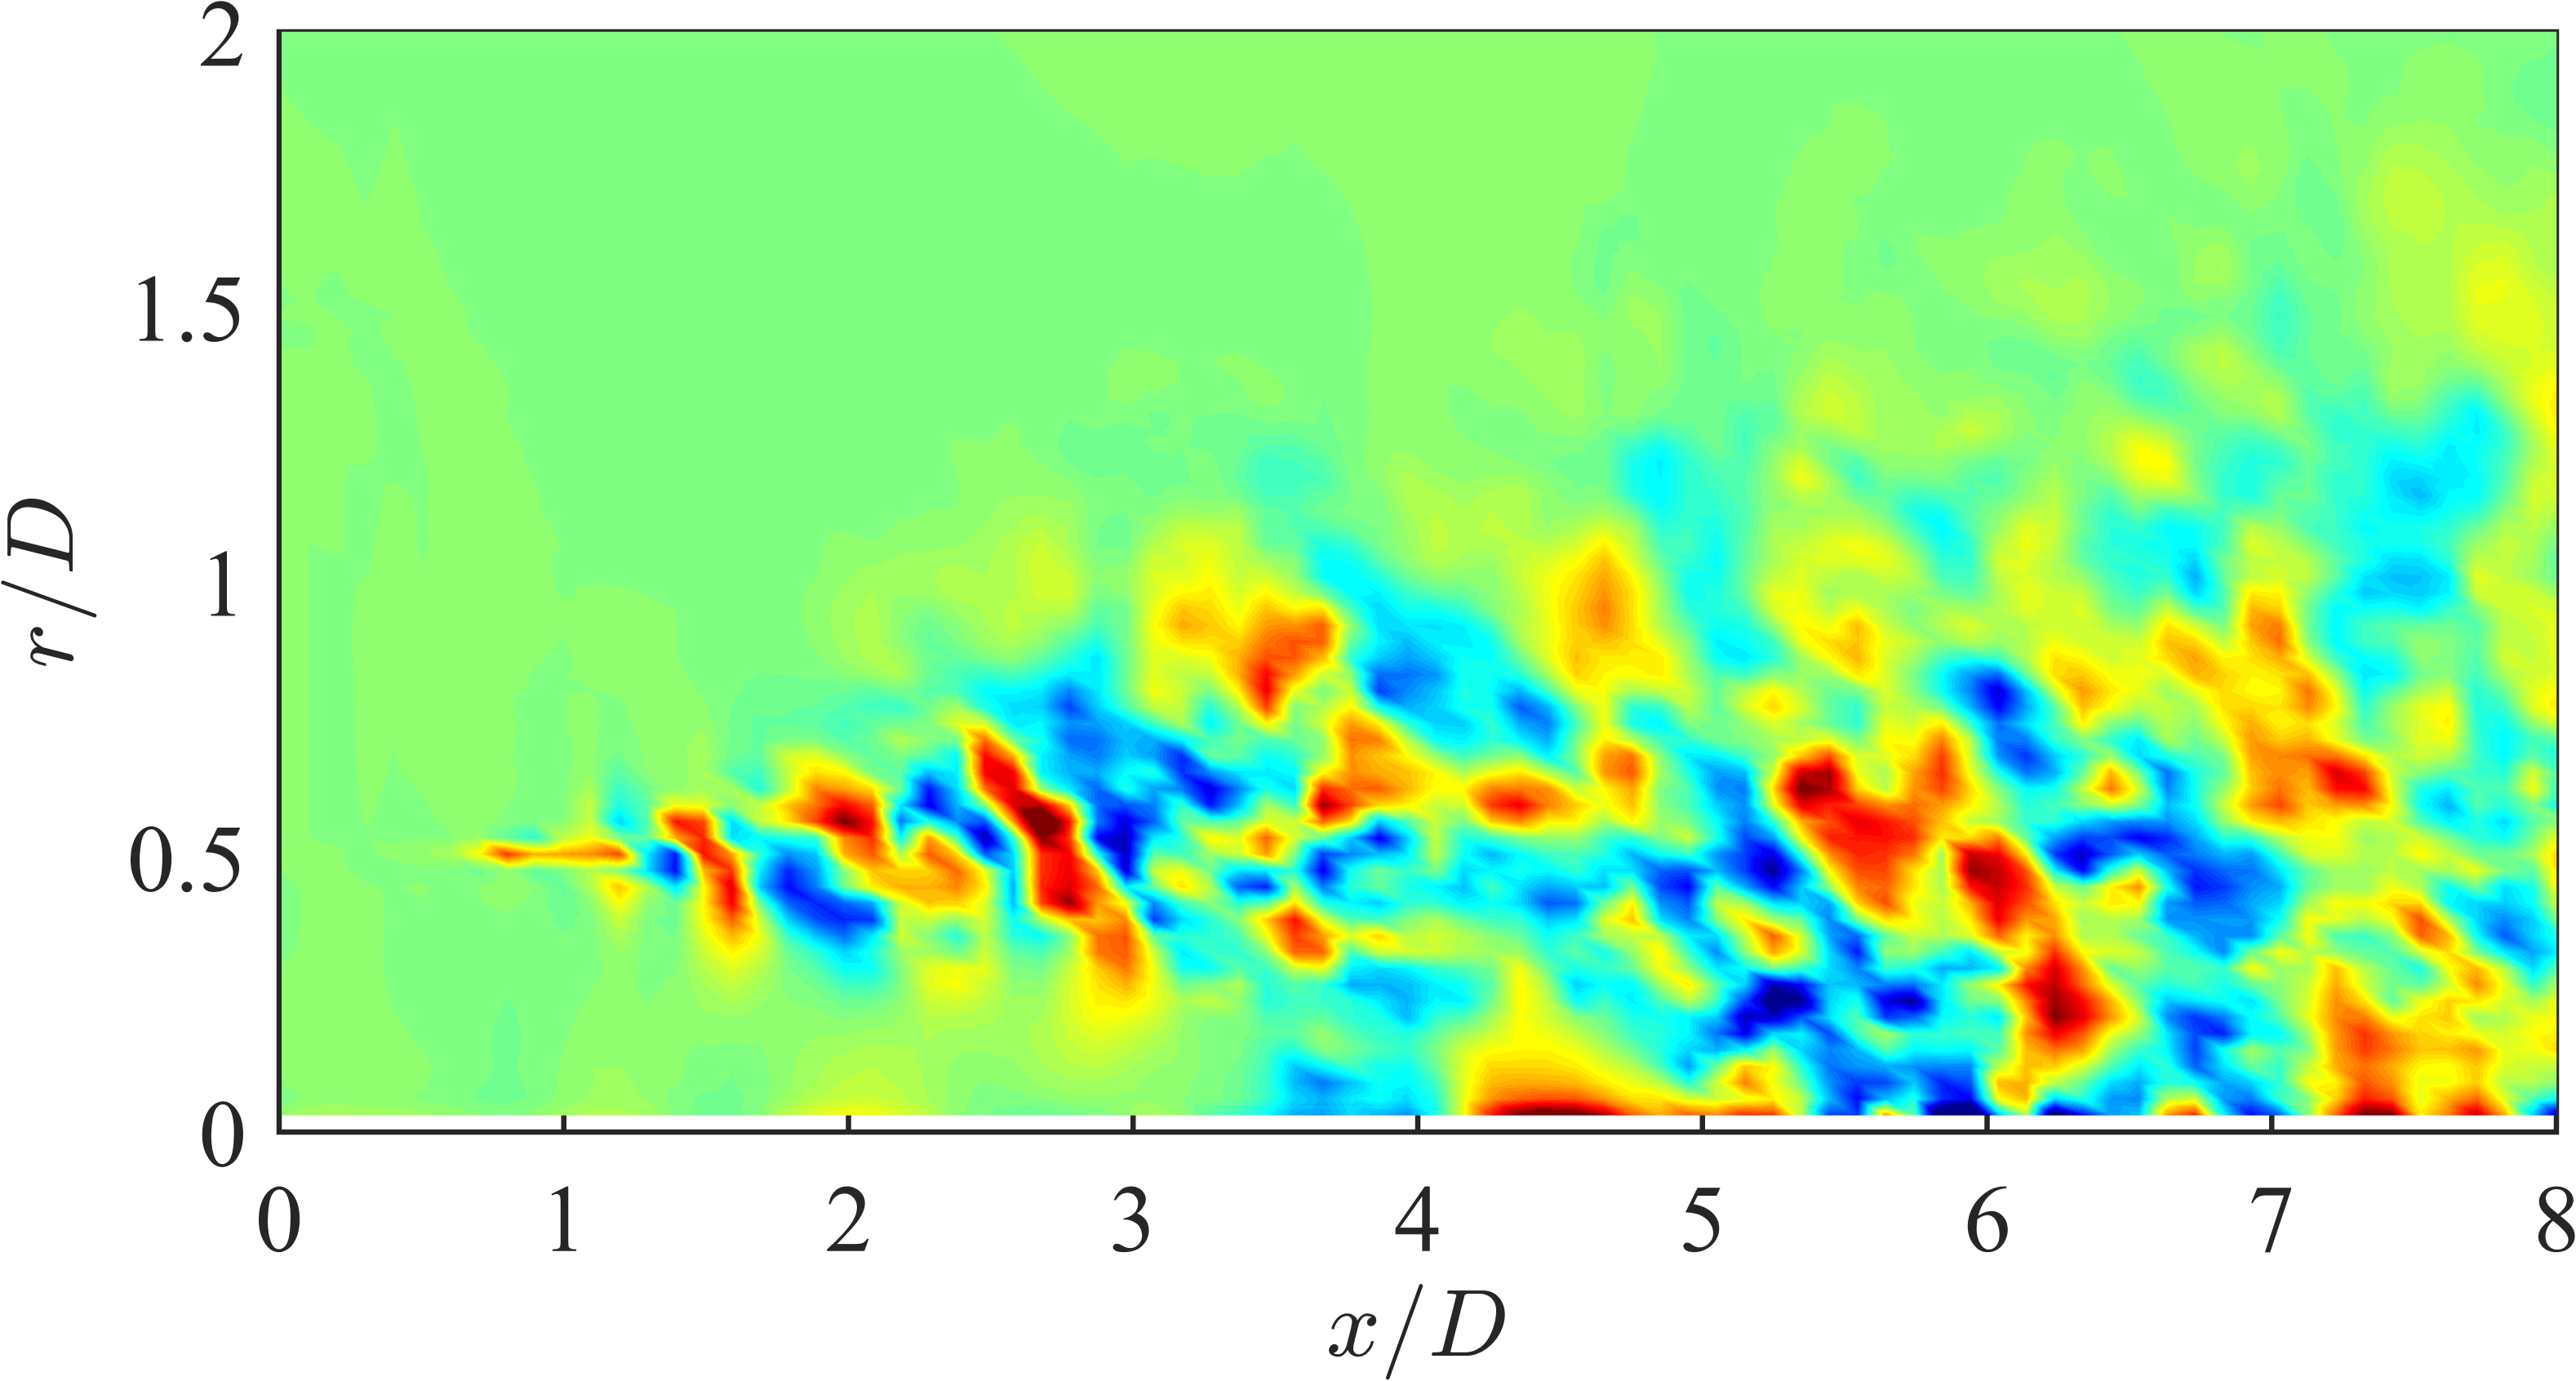
\includegraphics[width=0.95\linewidth]{Figures/LES_3CDil.png}
%		\caption{}
%	\end{subfigure}
%	\caption{Dilatation computed using only the axial and radial components (a) and computed using the full three-component velocity vector (b); a uniform colorscale has been used for the two plots.}
%	\label{fig:LES_streamwise_dil}
%\end{figure}
%
%The solution procedure is therefore to first compute $\Phi$ using \eq{eq:helmholtz}, then subtract the gradient of this field (the potential velocity field) from the raw velocity vector field in order to produce the solenoidal velocity field. 
%This was done using a standard, second-order accurate centered finite difference scheme by Taylor approximation.
%A relatively low-order approximation to the spatial derivatives was deemed sufficient for this particular work, as the spatial grid was very fine compared to the wavelength of the dominant structures under investigation.
%For reference, $l/ds \simeq 30$, where $l$ is the average characteristic length of the excited large-scale structures near the end of the potential core and $ds$ is the grid spacing ($ds = 0.6$ mm).
%
%As the flow has already been assumed to be axisymmetric, the Poisson equation is solved over the top half of the jet only.
%(The top plane was chosen as the microphone tips are visible in the lower plane, which produced spurious vectors in the shear layer.)
%At the lower boundary (jet centerline), a zero-normal-gradient boundary condition was used to enforce axisymmetry.
%At the radial boundary, the solenoidal component was set to zero (as there is no turbulent flow in this region, and the only outgoing waves will be compressible).
%At the inflow and outflow however, the proper boundary conditions are not immediately obvious.
%Other researchers using numerical databases \citep{Unnikrishnan2015} have argued that the solenoidal component be set to zero here as the turbulent eddies have either not grown to significant values or decay to insignificant values at these locations, respectively.
%For the domain explored in the current work however, this does not appear to be necessarily accurate, and instead the \textit{potential} component is set to zero at both the inlet and outlet.
%At the outflow boundary ($x/D \simeq 13$), there is still significant vortical behavior, but the Mach number is relatively low ($M_j \simeq 0.5$) and hence compressibility is expected to be negligible.
%At the inflow boundary (which is $\sim1.4$ mm downstream of the nozzle exit), the solenoidal component is clearly not negligible in the shear layer region (since $\partial U_x / \partial r \neq 0$).
%If the inflow is approximated as a plug flow (which the ensemble-averaged PIV indicates is not entirely unreasonable for the experimental grid), $\partial U_x / \partial x = \partial U_r / \partial r = 0$ and hence the potential component is negligible here.
%Therefore, the potential component was set to zero at both the inlet and outlet.
%Second-order accurate centered finite differences were again used to approximate the derivatives in the boundary conditions; a single ghost node was used along each boundary to enforce these conditions.
%
%Sample results from the experimental database for this procedure have been provided in \fig{fig:valid_helmholtz}.
%Here, the axial and radial velocity components for the original (estimated) and decomposed velocity fields are shown for $St_{DF}=0.05$.
%From the raw velocity field, a single large-scale structure is readily identifiable at $x/D \simeq 6$ (which is the end of the potential core).
%Due to the very low frequency of the excitation (impulsive forcing), no other large-scale structures are clearly visible in the flow-field.
%As expected, the Helmholtz decomposition produces a solenoidal velocity that is quite similar to the full velocity field; even at high subsonic Mach numbers, compressibility plays a minor (though definitely non-negligible) role in the overall evolution of the shear layer and potential core.
%The potential (compressible) velocity field does exhibit coherent axial and radial velocity fluctuations which correspond to the large-scale structure; in fact, the potential and solenoidal velocity fluctuations associated with the large-scale structure are of similar magnitude, suggesting that compressibility is important for the development of the large-scale structure themselves.
%
%The upstream development of the potential field, in which no large-amplitude oscillations are observed, validates the assumption of plug flow made in the boundary conditions.
%In contrast, non-negligible fluctuations are observed near the outflow boundary; unfortunately, the experimental domain does not extend far enough downstream for the compressible component to fully decay.
%However, the potential component is still far weaker than the solenoidal component.
%For validation purposes, the boundary conditions of Unnikrishnan \& Gaitonde \citep{Unnikrishnan2015} (zero solenoidal component at the inflow and outflow) were also implemented and compared against the current results.
%Though not shown here for brevity, the zero-solenoidal boundary conditions produced similar fields at the interior of the domain, but non-physical oscillations at the inflow and outflow boundaries.
%Based on these results, the zero-potential boundary conditions were retained; though there is a discrepancy between the boundary conditions and the physical system at the outflow boundary, the numerical effects of this are expected to be minor.
%\begin{figure}
%	\centering
%	\begin{subfigure}{0.5\textwidth}
%		\centering
%		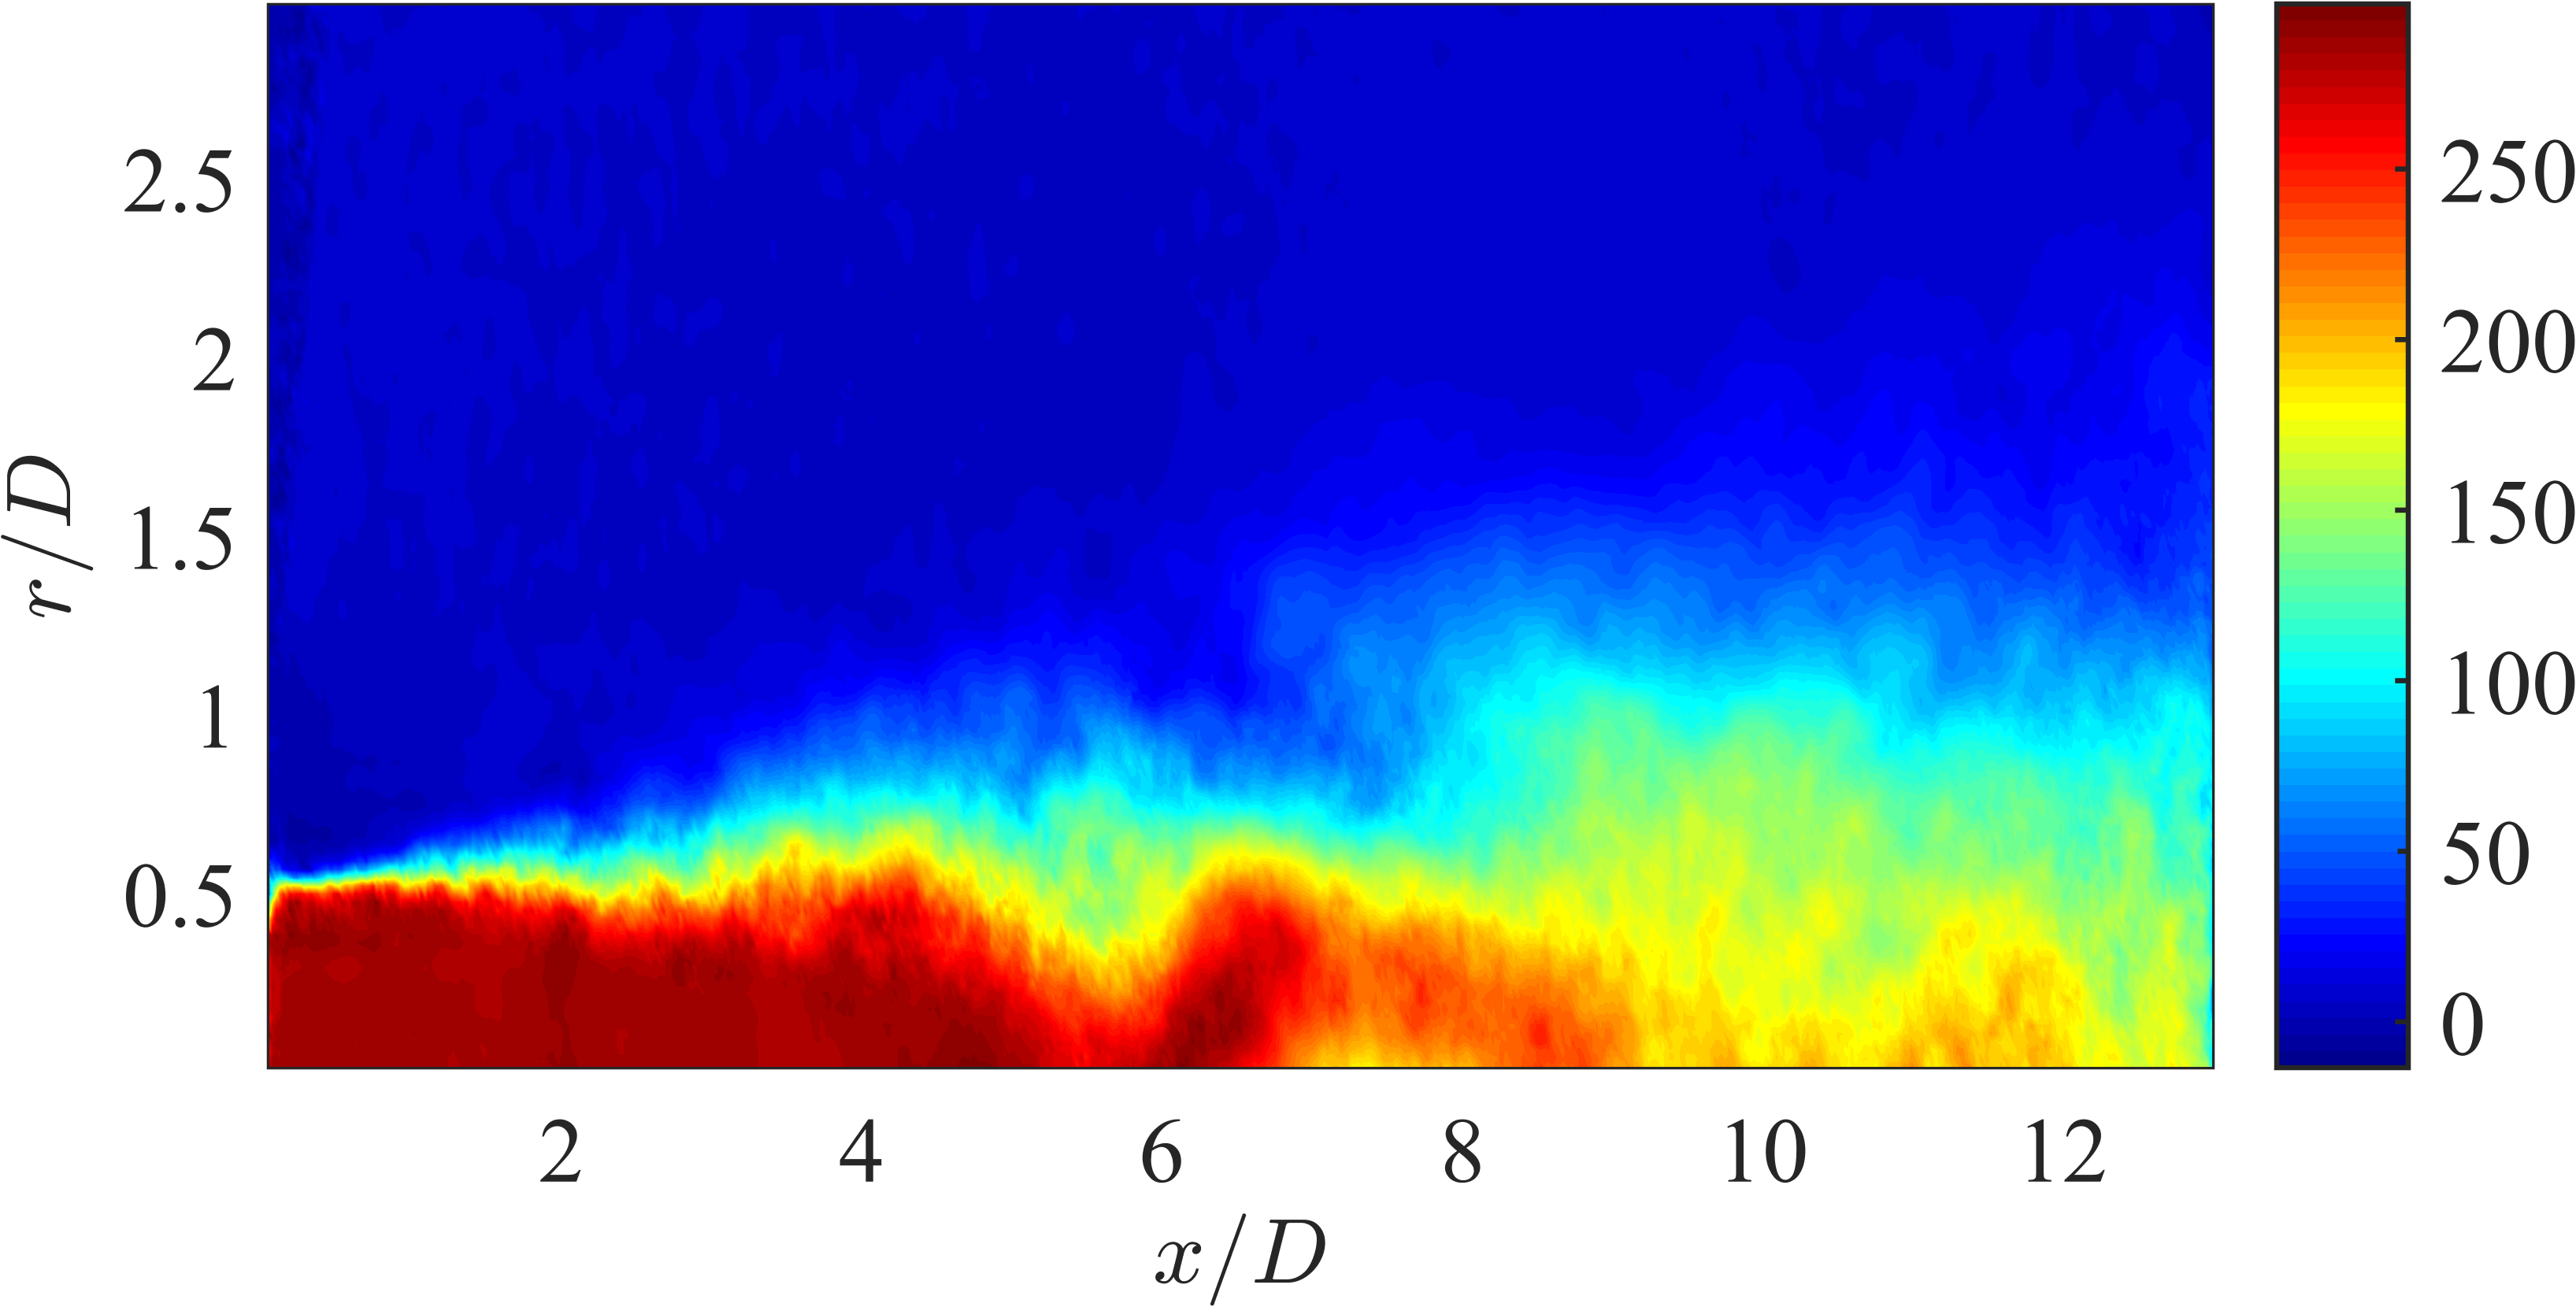
\includegraphics[width=0.95\linewidth]{Figures/ch5_valid_Inst_Uz.png}
%		\caption{}
%	\end{subfigure}%
%	\begin{subfigure}{0.5\textwidth}
%		\centering
%		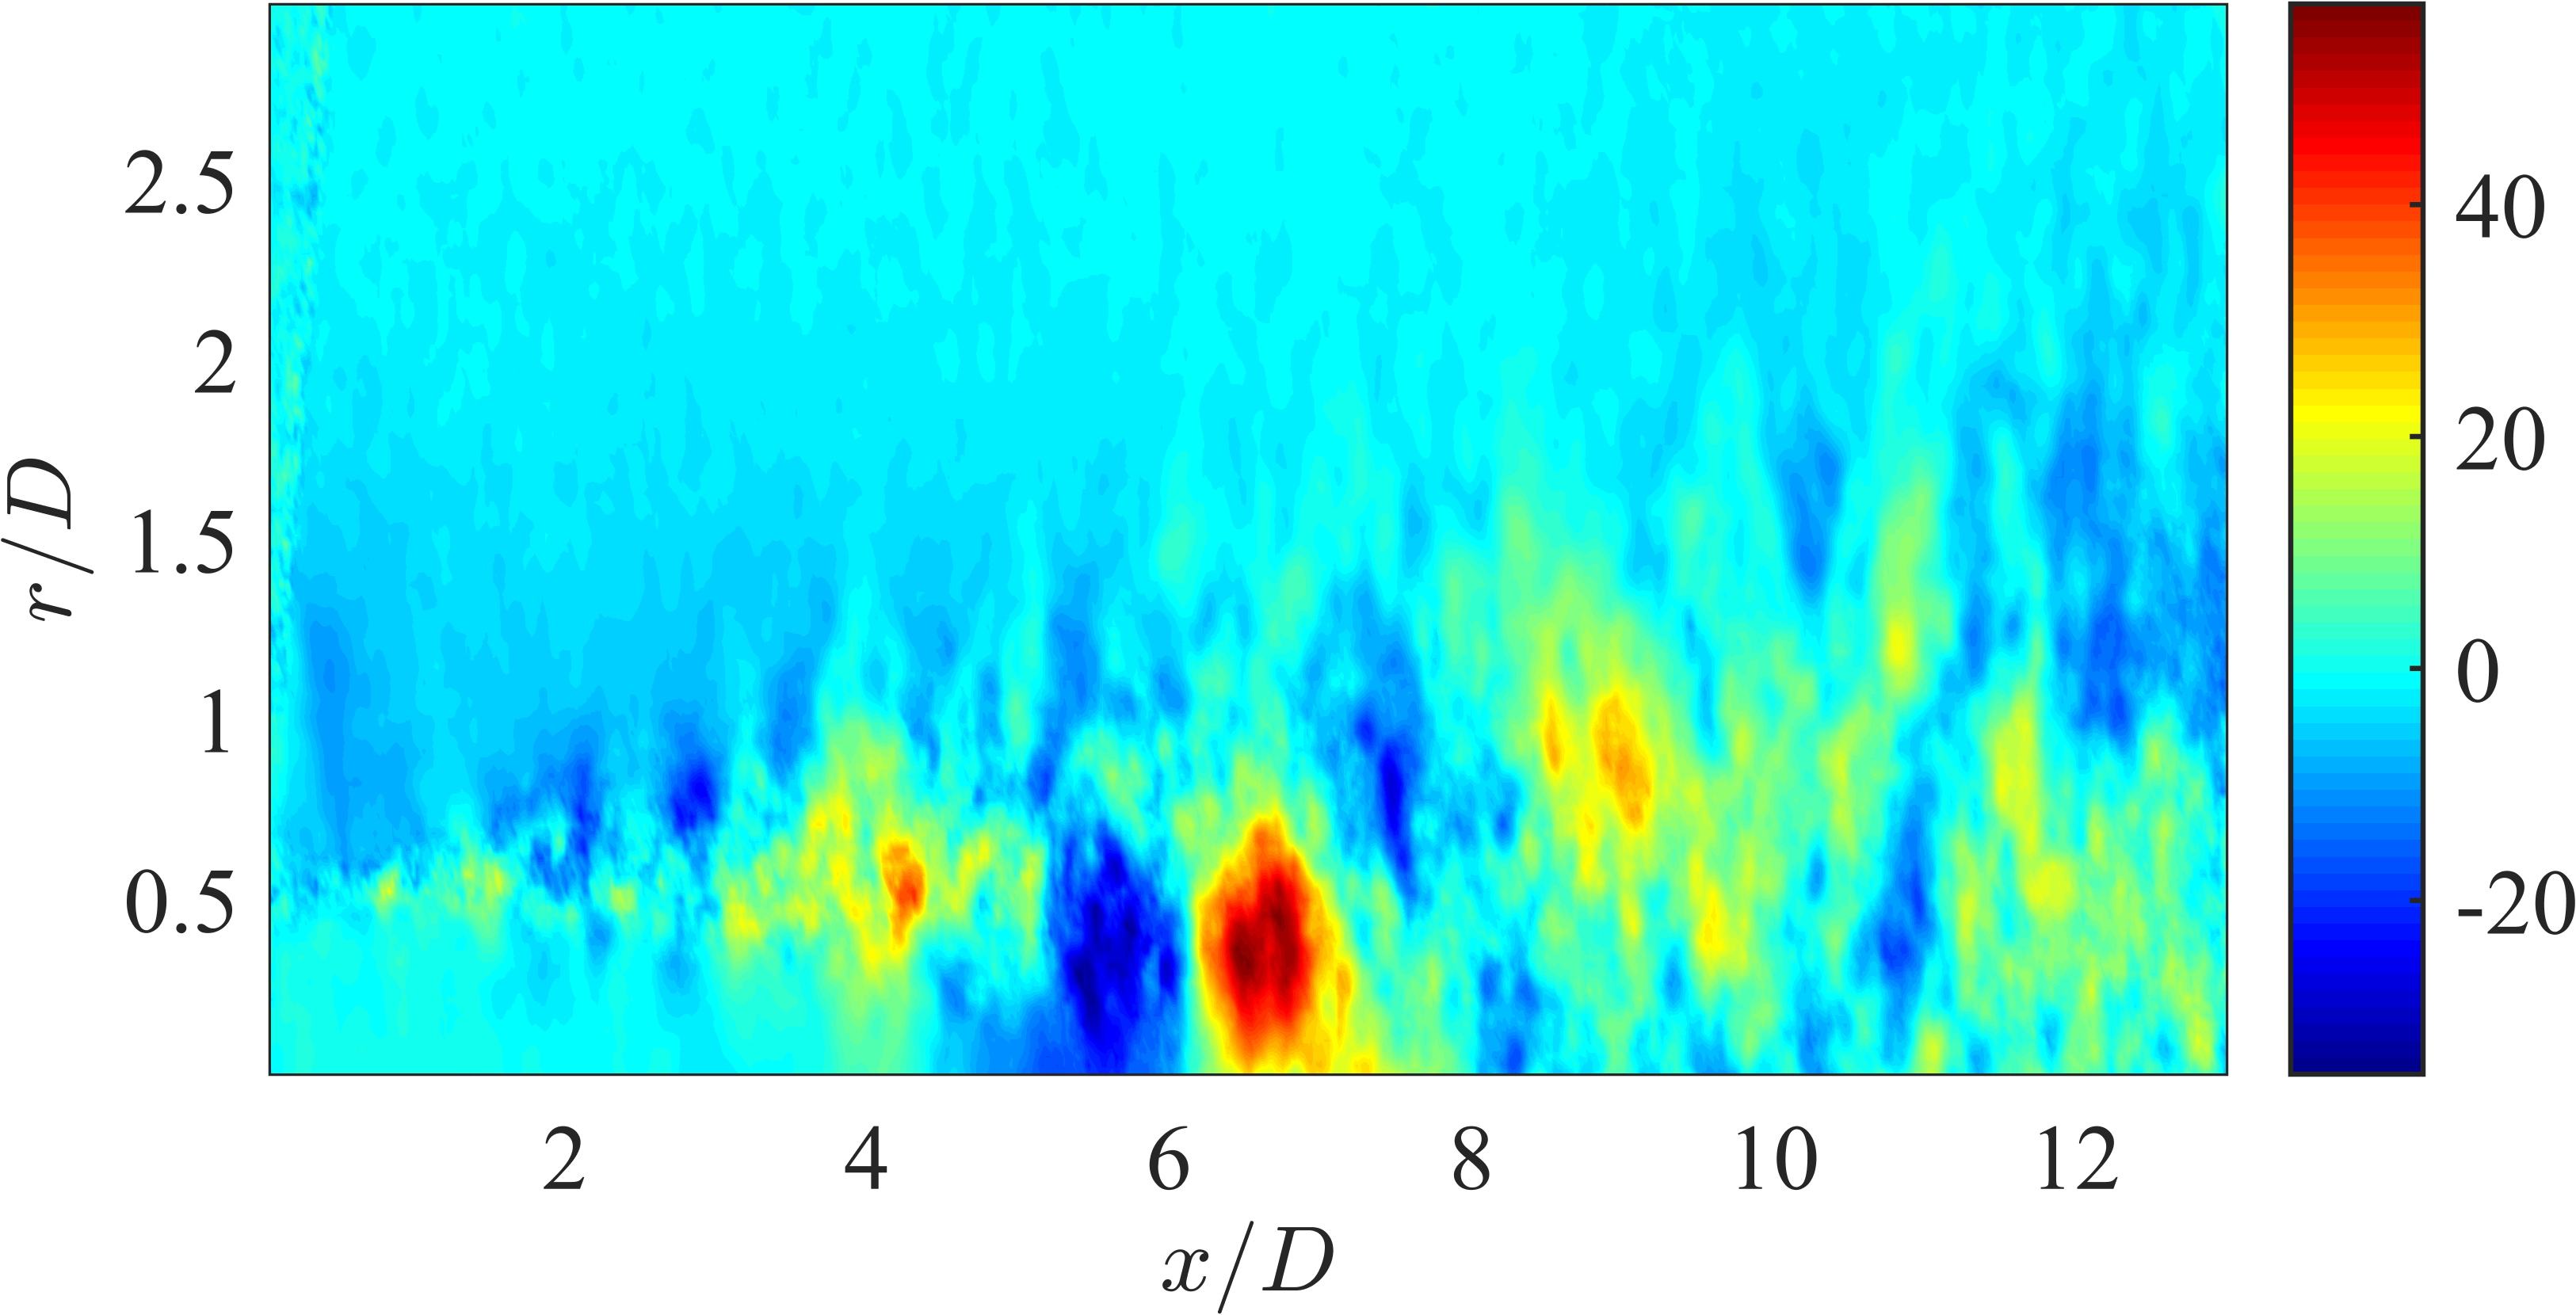
\includegraphics[width=0.95\linewidth]{Figures/ch5_valid_Inst_Ur.png}
%		\caption{}
%	\end{subfigure}\\
%	\begin{subfigure}{0.5\textwidth}
%		\centering
%		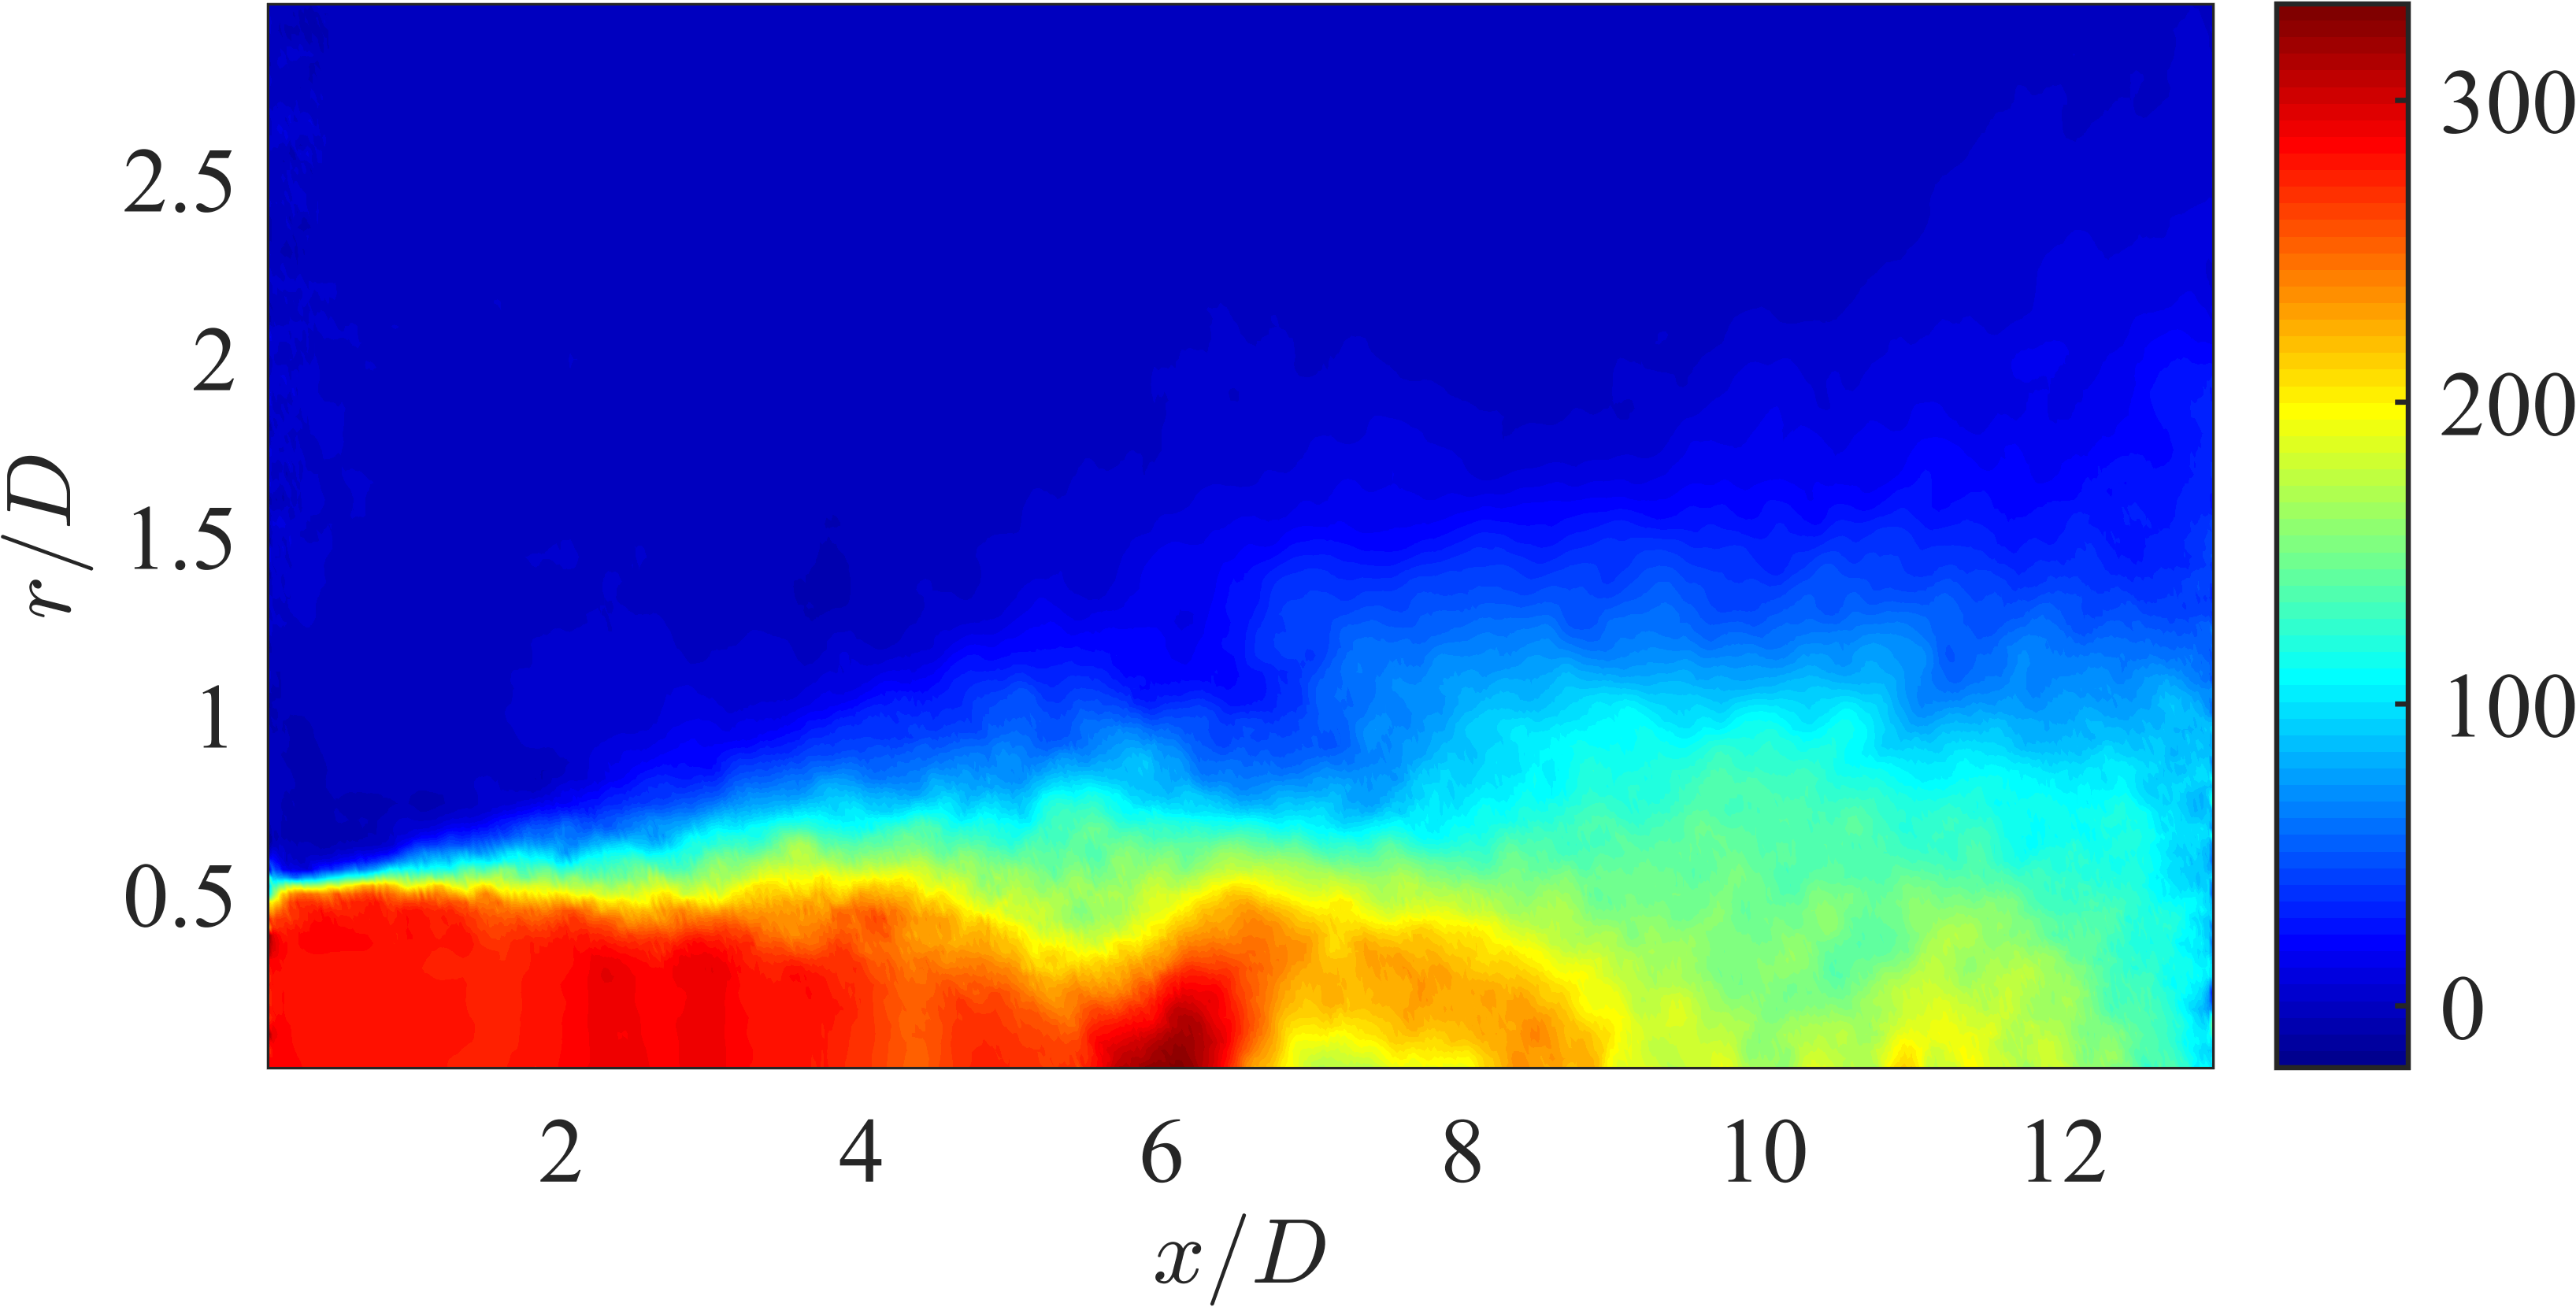
\includegraphics[width=0.95\linewidth]{Figures/ch5_valid_Inst_solUz.png}
%		\caption{}
%	\end{subfigure}%
%	\begin{subfigure}{0.5\textwidth}
%		\centering
%		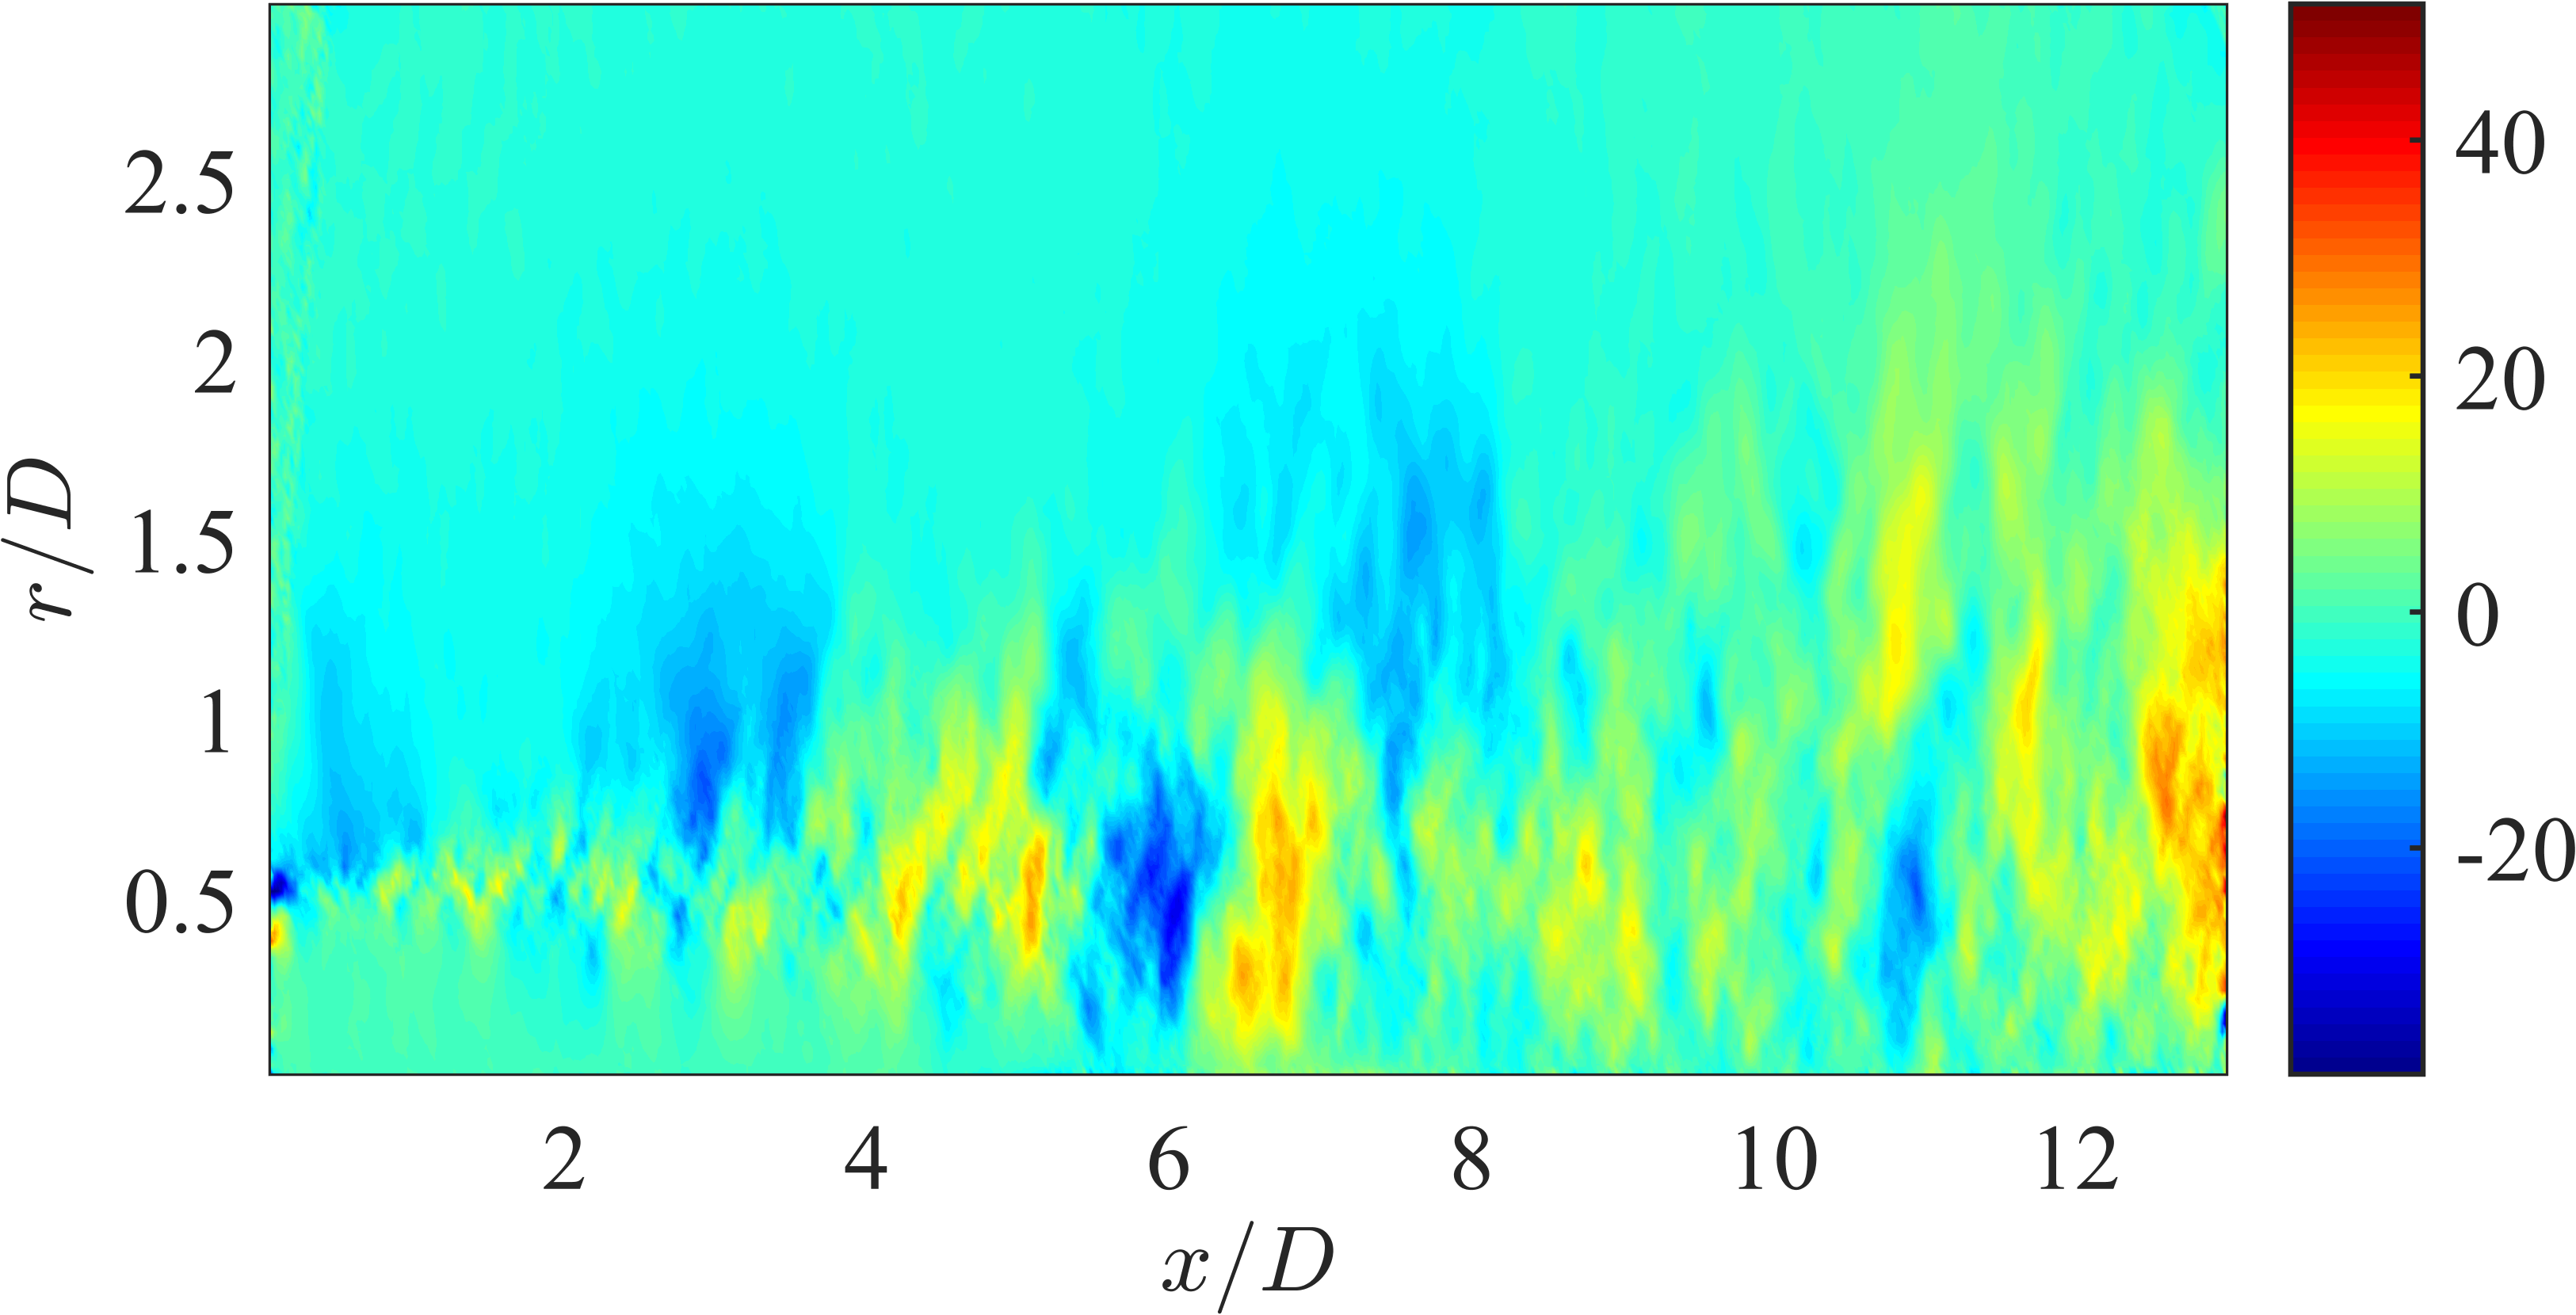
\includegraphics[width=0.95\linewidth]{Figures/ch5_valid_Inst_solUr.png}
%		\caption{}
%	\end{subfigure}\\
%	\begin{subfigure}{0.5\textwidth}
%		\centering
%		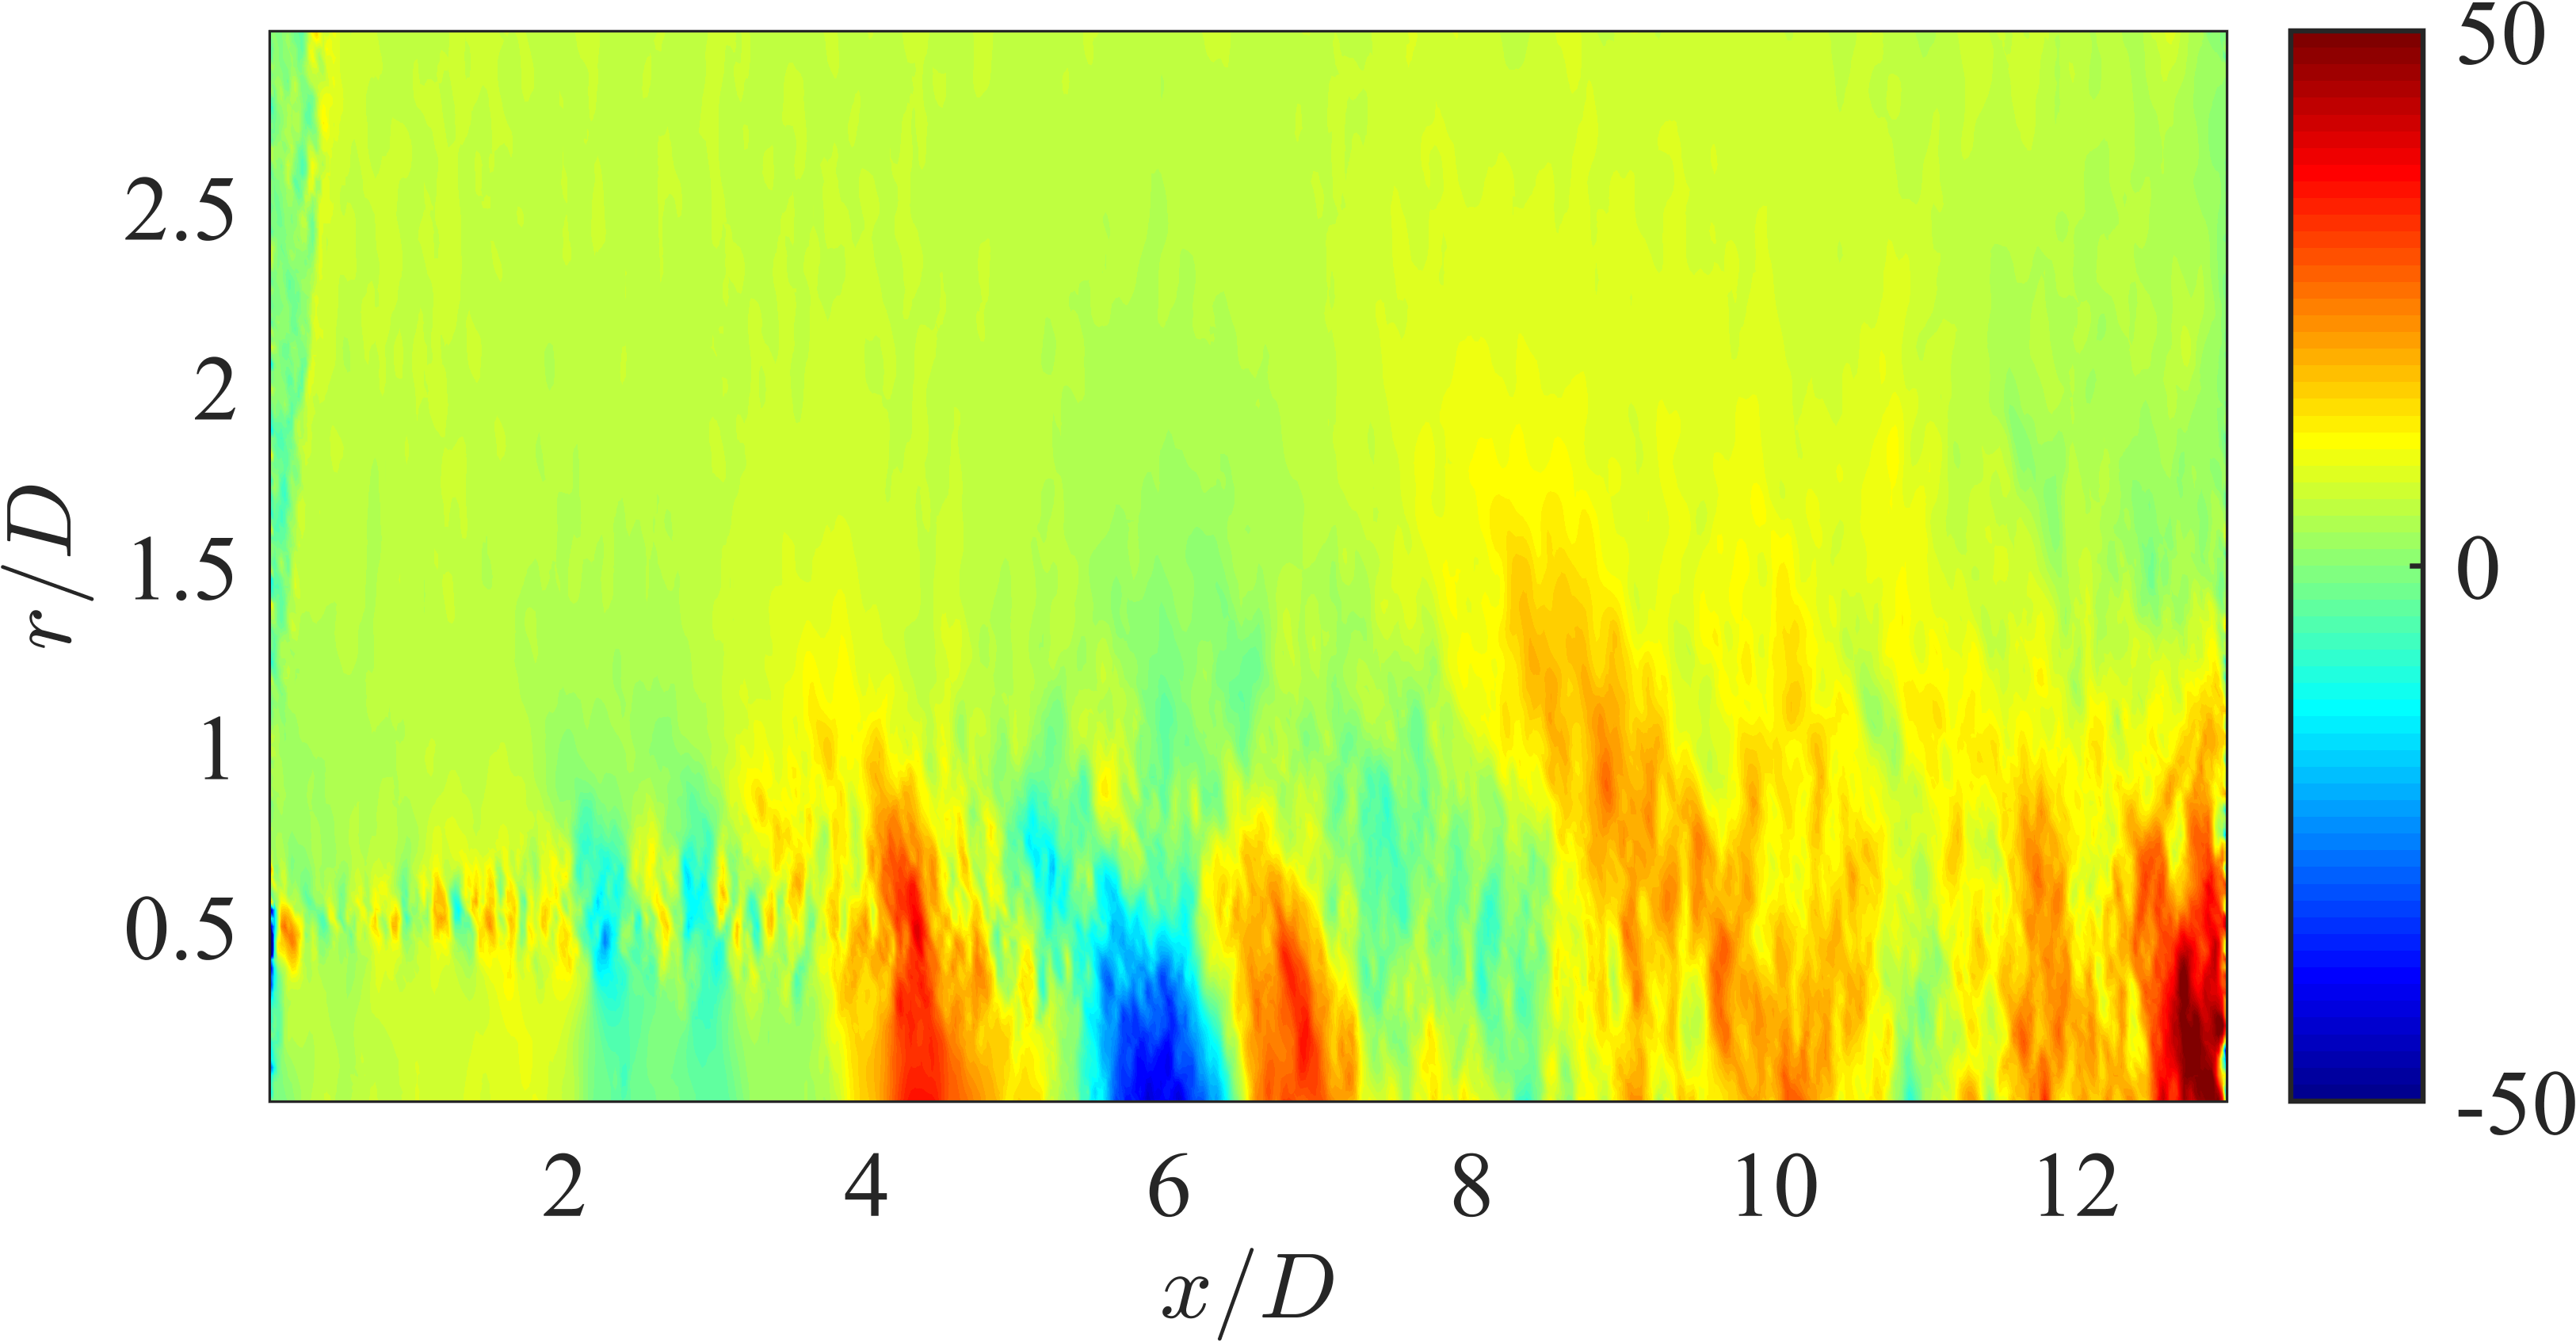
\includegraphics[width=0.95\linewidth]{Figures/ch5_valid_Inst_potUz.png}
%		\caption{}
%	\end{subfigure}%
%	\begin{subfigure}{0.5\textwidth}
%		\centering
%		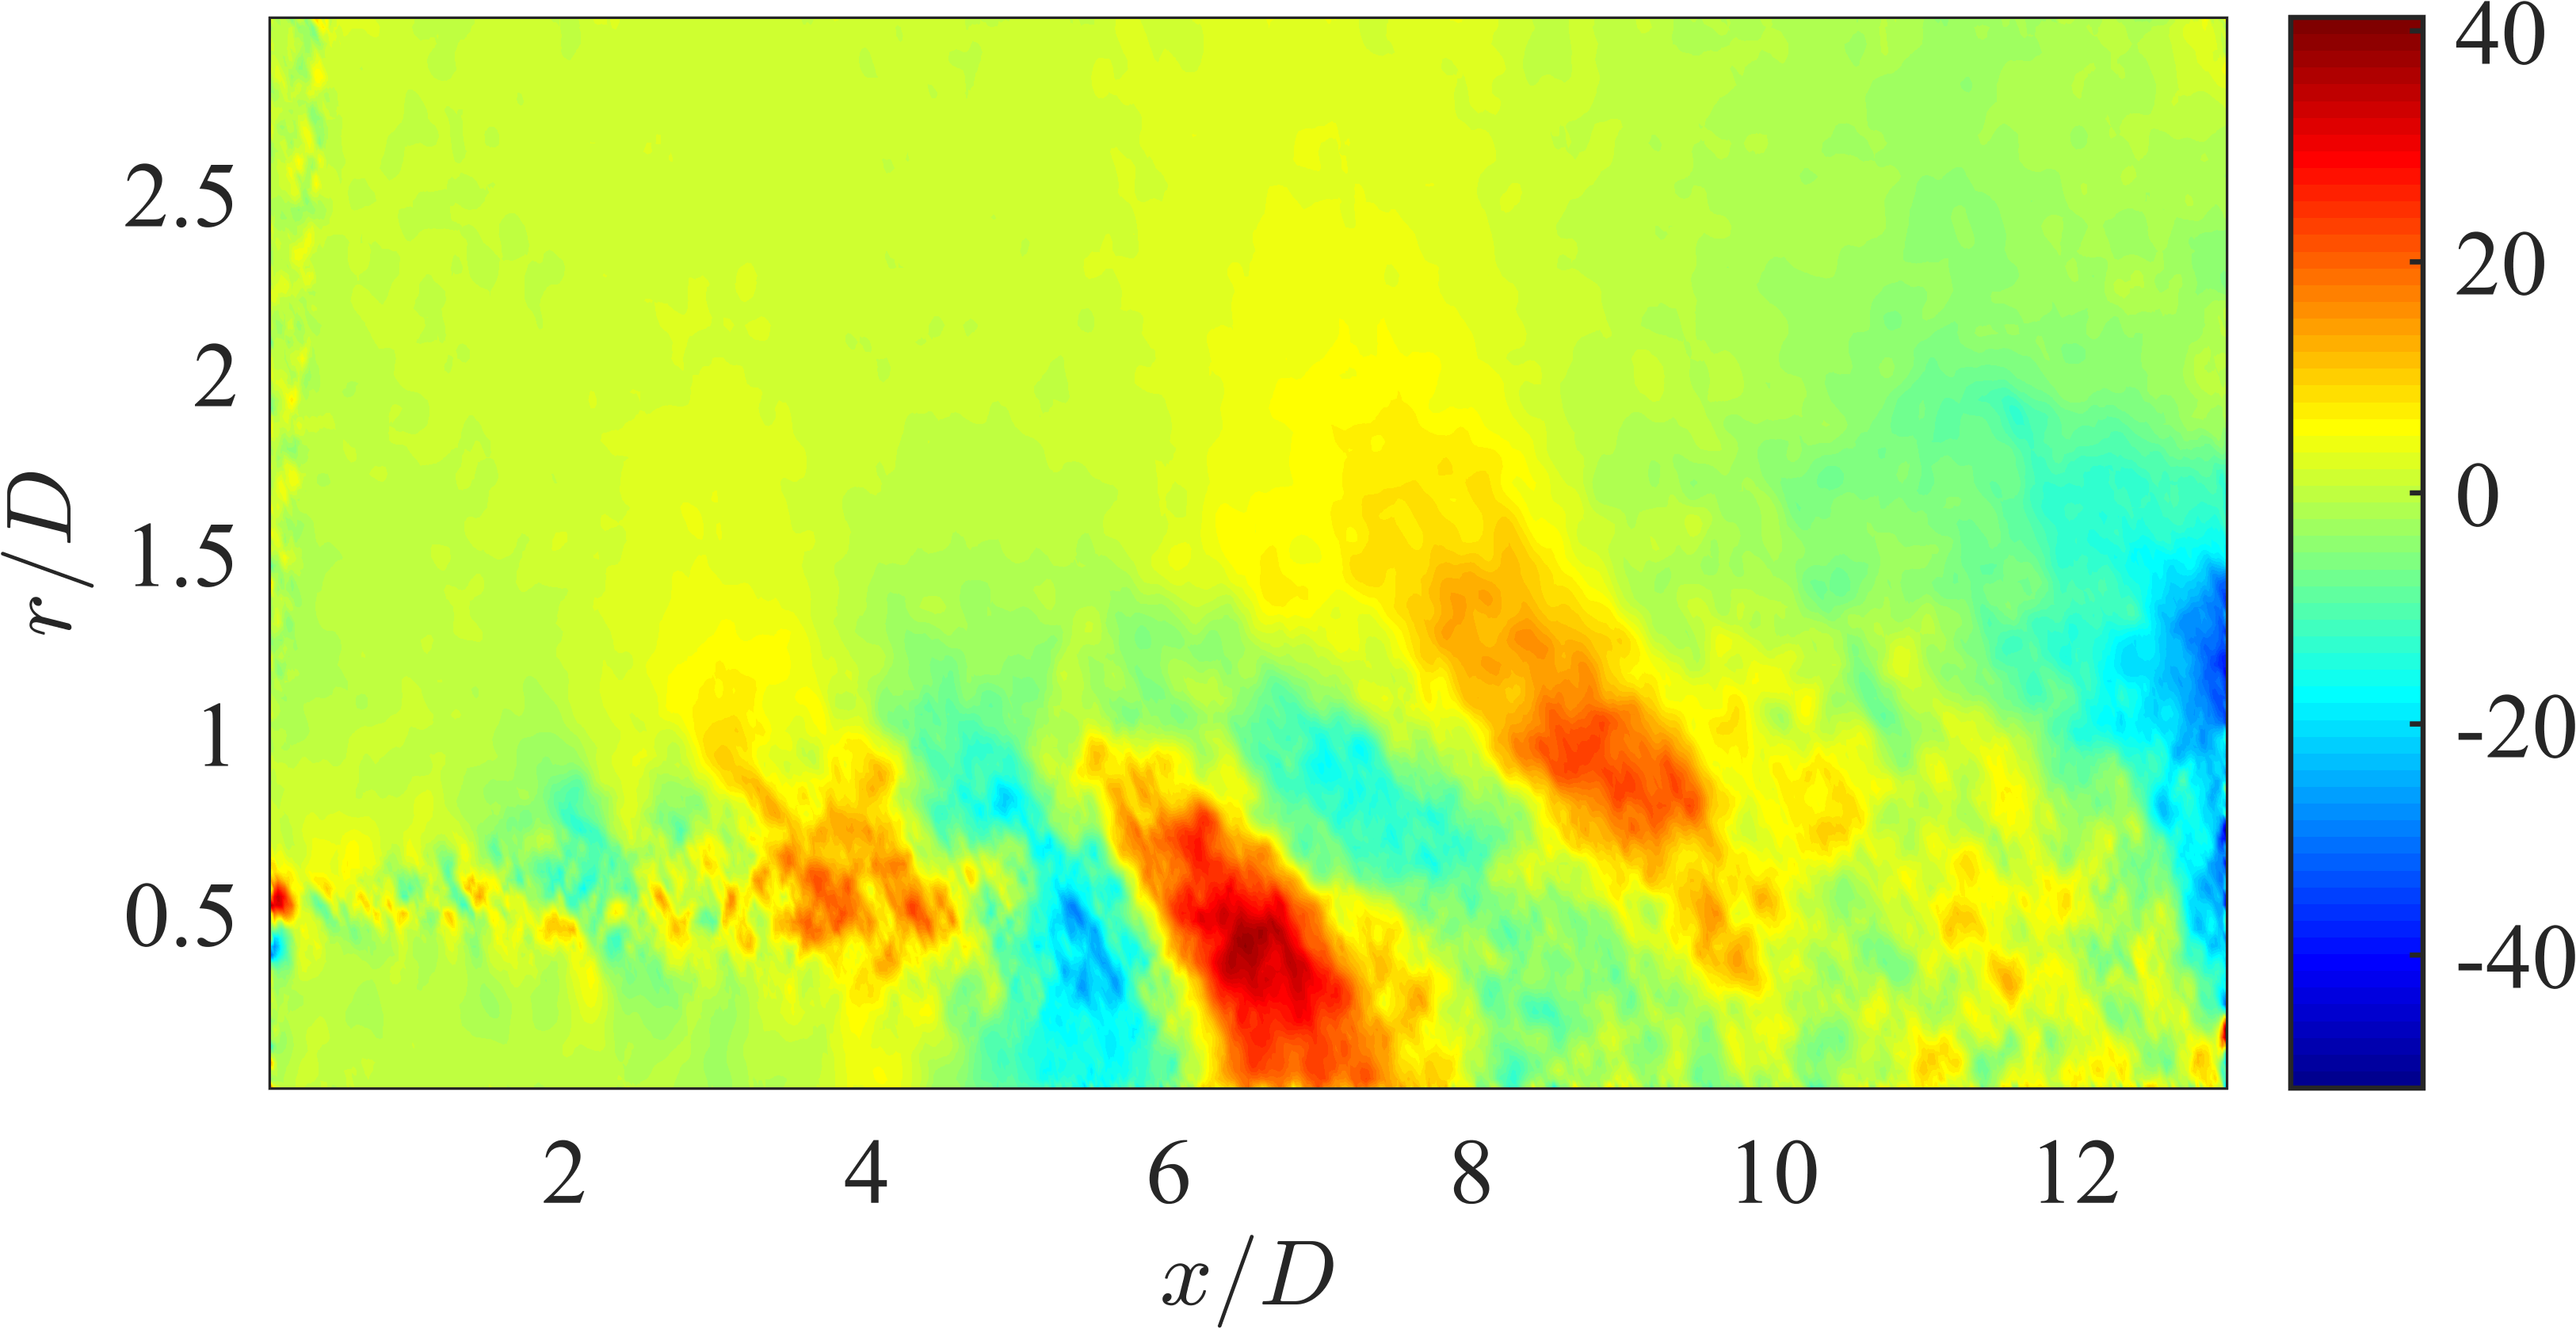
\includegraphics[width=0.95\linewidth]{Figures/ch5_valid_Inst_potUr.png}
%		\caption{}
%	\end{subfigure}
%	\caption{Instantaneous axial (a,c,e) and radial (b,d,f) velocity components for the original (a,b), solenoidal (c,d), and potential (e,f) velocity fields (units in m/s), for $St_{DF} = 0.05.$}
%	\label{fig:valid_helmholtz}
%\end{figure}
%
%\subsubsection{Pseudo-Pressure Solver}
%Once the solenoidal velocity field is known, the fluctuating pseudo-sound field can be computed as the incompressible solution to the momentum and continuity equations (\eq{eq:solenoidal_pressure}).
%The source field is calculated explicitly from the solution of the Helmholtz decomposition (that is, the double divergence of the incompressible velocity stress tensor) using second-order accurate finite differences.
%As with the preceding Poisson equation, the azimuthal terms in this second Poisson equation are assumed negligible in comparison to the radial and axial terms and are thus ignored.
%Again, as done previously for the Helmholtz decomposition, the governing equation is approximated using second-order accurate centered finite differences, and ghost nodes are used at the domain boundaries to enforce the boundary conditions.
%
%The hydrodynamic pressure field has been observed to strongly decay with radial position \citep{Arndt1997}; given the radial extent of the experimental domain, it was therefore assumed that the pseudo-sound fluctuations have decayed to negligible values by the time they reach the upper domain boundary.
%In accordance with the boundary assumptions made in the preceding section, at the inflow boundary plug flow has again been assumed, meaning that the pseudo-pressure \textit{fluctuations} are negligible at the inlet. 
%The outflow boundary was assumed to be far enough downstream such that the fluctuations were also negligible at the boundary.
%Finally, the lower boundary enforced the zero-normal-gradient required by the assumption of axisymmetry.
%
%Sample results for the pseudo-pressure field are shown in \fig{fig:valid_pseudopressure}, which corresponds to the solenoidal velocity decomposed in \fig{fig:valid_helmholtz}.
%As expected, a spatially-coherent fluctuation is observed coinciding with the location of the large-scale structure as identified in the velocity field.
%Lower-amplitude oscillations are also observed upstream of the end of the potential core, while downstream the fluctuations are fairly incoherent and low-amplitude.
%By the end of the experimental domain, the pseudo-pressure field has decayed to essentially negligible values.
%At the inlet however, a large-amplitude pressure sink resides along the jet lipline and extends for $x/D \lesssim 0.5$.
%The origin of this pressure sink is not clear to the researcher, however it is entirely numerical in nature; as will be seen in the following section, the consistency of this sink results in no superfluous aeroacoustic source being computed for this location.
%While the presence of this numerical error is unfortunate, given that it was not found to have a major effect on the computed aeroacoustic source field (which is ultimately the goal of this analysis), further inquiry into the cause of this numerical error was deemed unproductive.
%\begin{figure}
%	\centering
%	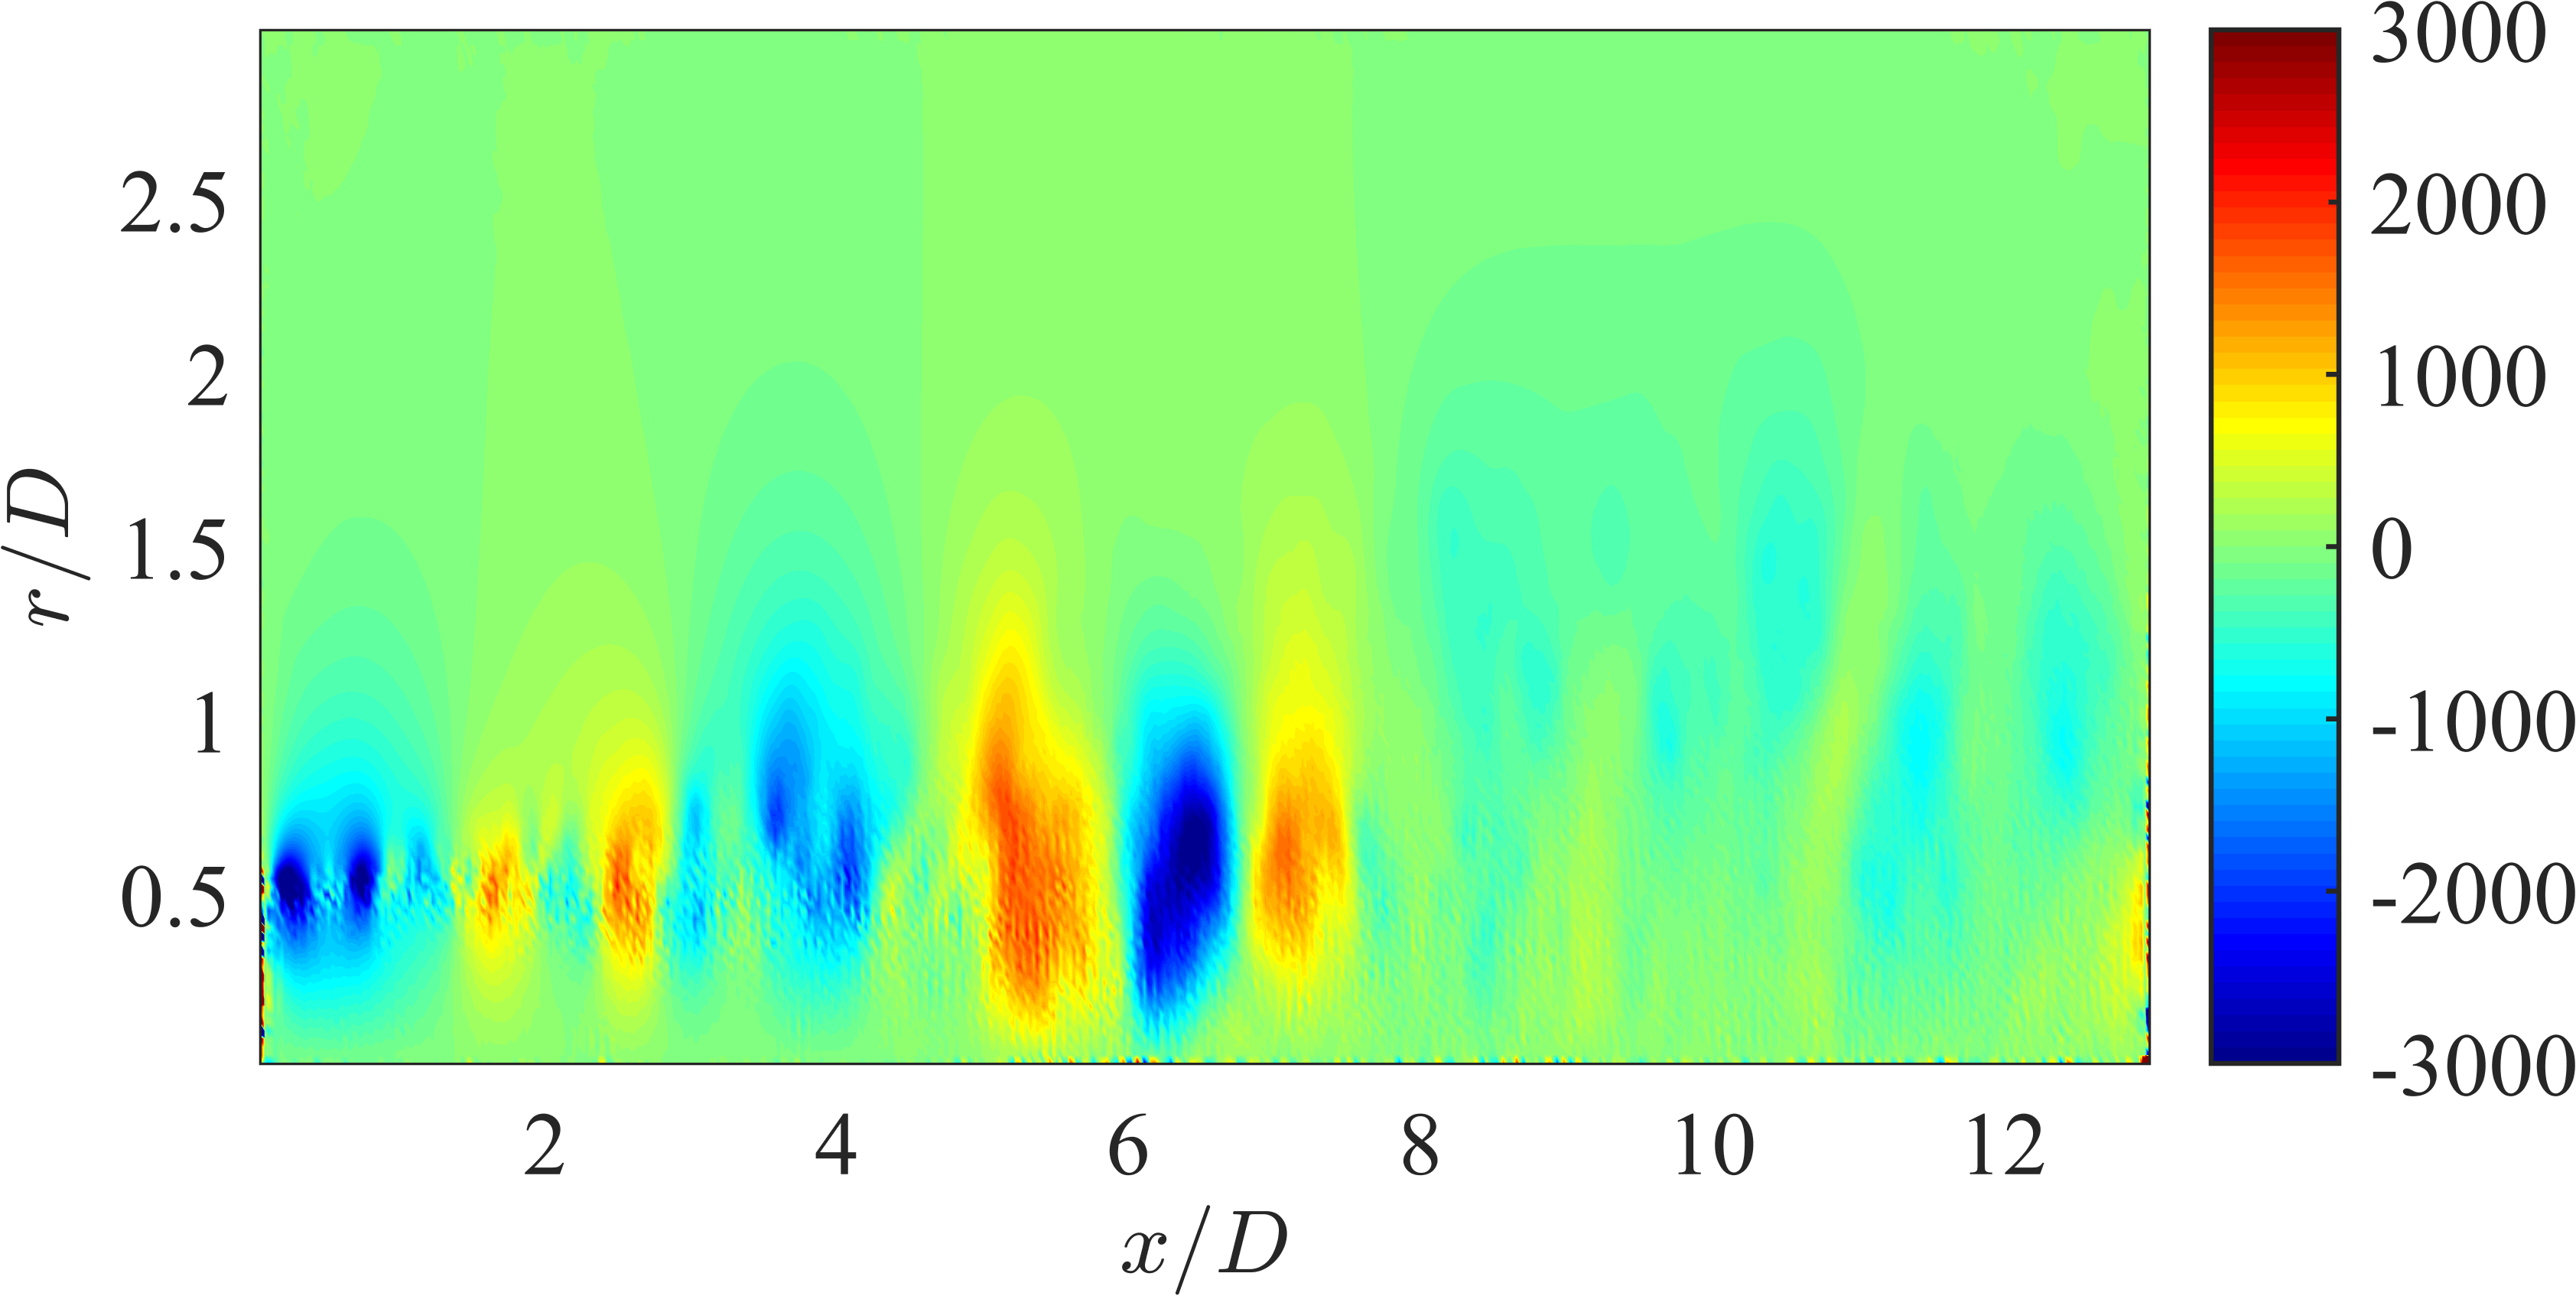
\includegraphics[width = 3.5in]{Figures/ch5_valid_Inst_ps.png}
%	\caption{Instantaneous pseudo-pressure field for the same conditions as \fig{fig:valid_helmholtz}.}
%	\label{fig:valid_pseudopressure}
%\end{figure}
%\subsubsection{Wavelet Denoising and Source Computation}
%The aeroacoustic source term can now be computed explicitly as the second temporal derivative of the pseudo-sound field (\eq{eq:ribner_source}).
%However, filtering of the pseudo-pressure field along the temporal dimension was found to be necessary before computation of the derivative, due to the accumulation of experimental and numerical error.
%As discussed by Farge \citep{Farge1992}, unlike the Fourier transform coefficients which are well-localized in frequency but completely delocalized in time, the wavelet transform coefficients are well-localized in both frequency and time. 
%As a result, a truncated set of the wavelet coefficients will better preserve the temporal characteristics of a given signal than a truncated set of Fourier coefficients.
%Hence, wavelet-based filtering was used to remove the influence of the experimental/numerical errors; more specifically, an energy threshold was applied to the orthogonal wavelet coefficients in order to remove the less-energetic, incoherent events from the pseudo-pressure field.
%Interested readers should see Donoho \& Johnstone [1994], Farge \etal [1999] and Ruppert-Felsot \etal [2009] for additional details on denoising using orthogonal wavelet transforms, including more advanced algorithms.
%
%For the current work, the fast orthogonal wavelet transforms implemented in Stanford University, Department of Statistics' \texttt{WaveLab 850} software library were utilized.
%The mother wavelet was defined as the $5^{th}$-order Battle-Lemarie wavelet; sample data was also analyzed using other smooth wavelets (high-order Coiflets and Symmlets) to ensure that the final results were not affected by the choice of mother wavelet.
%The orthogonal wavelet transform was performed along the temporal domain separately for each spatial location; the time-series was zero-padded so that it matched a dyadic grid.
%A soft energy threshold was used to separate the coherent, large-scale pressure fluctuations from the incoherent noise.
%In traditional wavelet-denoising, the threshold is often defined as $\epsilon = \sqrt{2 \sigma^2_n \mathrm{log}_e N}$, where $\sigma^2_n$ is the variance of the noise, and $N$ is the sample length.
%However, for the current work this threshold was found to be too lax, and so a much more aggressive energy threshold of $\epsilon = 8 \sigma_n \sqrt{ \mathrm{log}_e N}$ was used.
%This value was found by trial-and-error to be the lowest threshold which consistently removed all discontinuities in the temporal derivative of the pressure trace.
%The variance of the noise was estimated by median filtering, as provided by \texttt{WaveLab 850}.
%
%%In the work of Kearney-Fischer \etal \cite{Kearney-Fischer2013}, a pseudo-wavelet filter was used on the far-field signal at aft angles in order to extract the dominant, intermittent acoustic events which were believed to be related to the dominant, intermittent large-scale structures in the jet shear layer. 
%%In that work, an energy cutoff of $\epsilon = 1.5\sigma$ was used; here $\sigma^2$ corresponds instead to the variance of the \textit{signal} rather than the noise in the signal. 
%%Kearney-Fischer \etal found that a signal filtered in such a manner retained the relevant aspects of the far-field acoustic spectrum at shallow angles, in particular the dominant energy peak and strong roll-off at high and low frequencies.
%%Based on these results, a threshold of $\epsilon = 2\sigma$ was chosen for the current work (due to the low signal-to-noise ratio); for consistency, $\sigma$ was calculated over the entire field rather than at each individual point; the error (and hence, energy) did not scale with spatial location, resulting much lower signal-to-noise ratios at far radial and axial positions. 
%
%Sample results for the wavelet-denoising are shown in \fig{fig:valid_denoising} for $x/D=1.75$ at the jet lipline (as will be shown later, the sources are centered around the jet lipline upstream of the end of the potential core).
%Here, the source computed from the raw pseudo-pressure field has been plotted against the source computed from the pseudo-pressure field which has undergone the wavelet-denoising.
%A high-amplitude, relatively low-frequency compact waveform is observed in the pseudo-pressure field centered around $\tau U_j /D \simeq 2.25$; this is the hydrodynamic wave associated with the passaged of the large-scale structure observed in \fig{fig:valid_helmholtz}.
%While intuitively one would expect the temporal derivative of this compact waveform to dominate the source field, without filtering the source field is completely dominated instead by the high-frequency noise in the pseudo-pressure even though it is of comparably low amplitude.
%The wavelet-denoising eliminates this error however, and recovers the expected behavior for the second temporal derivative.
%\begin{figure}
%	\centering
%	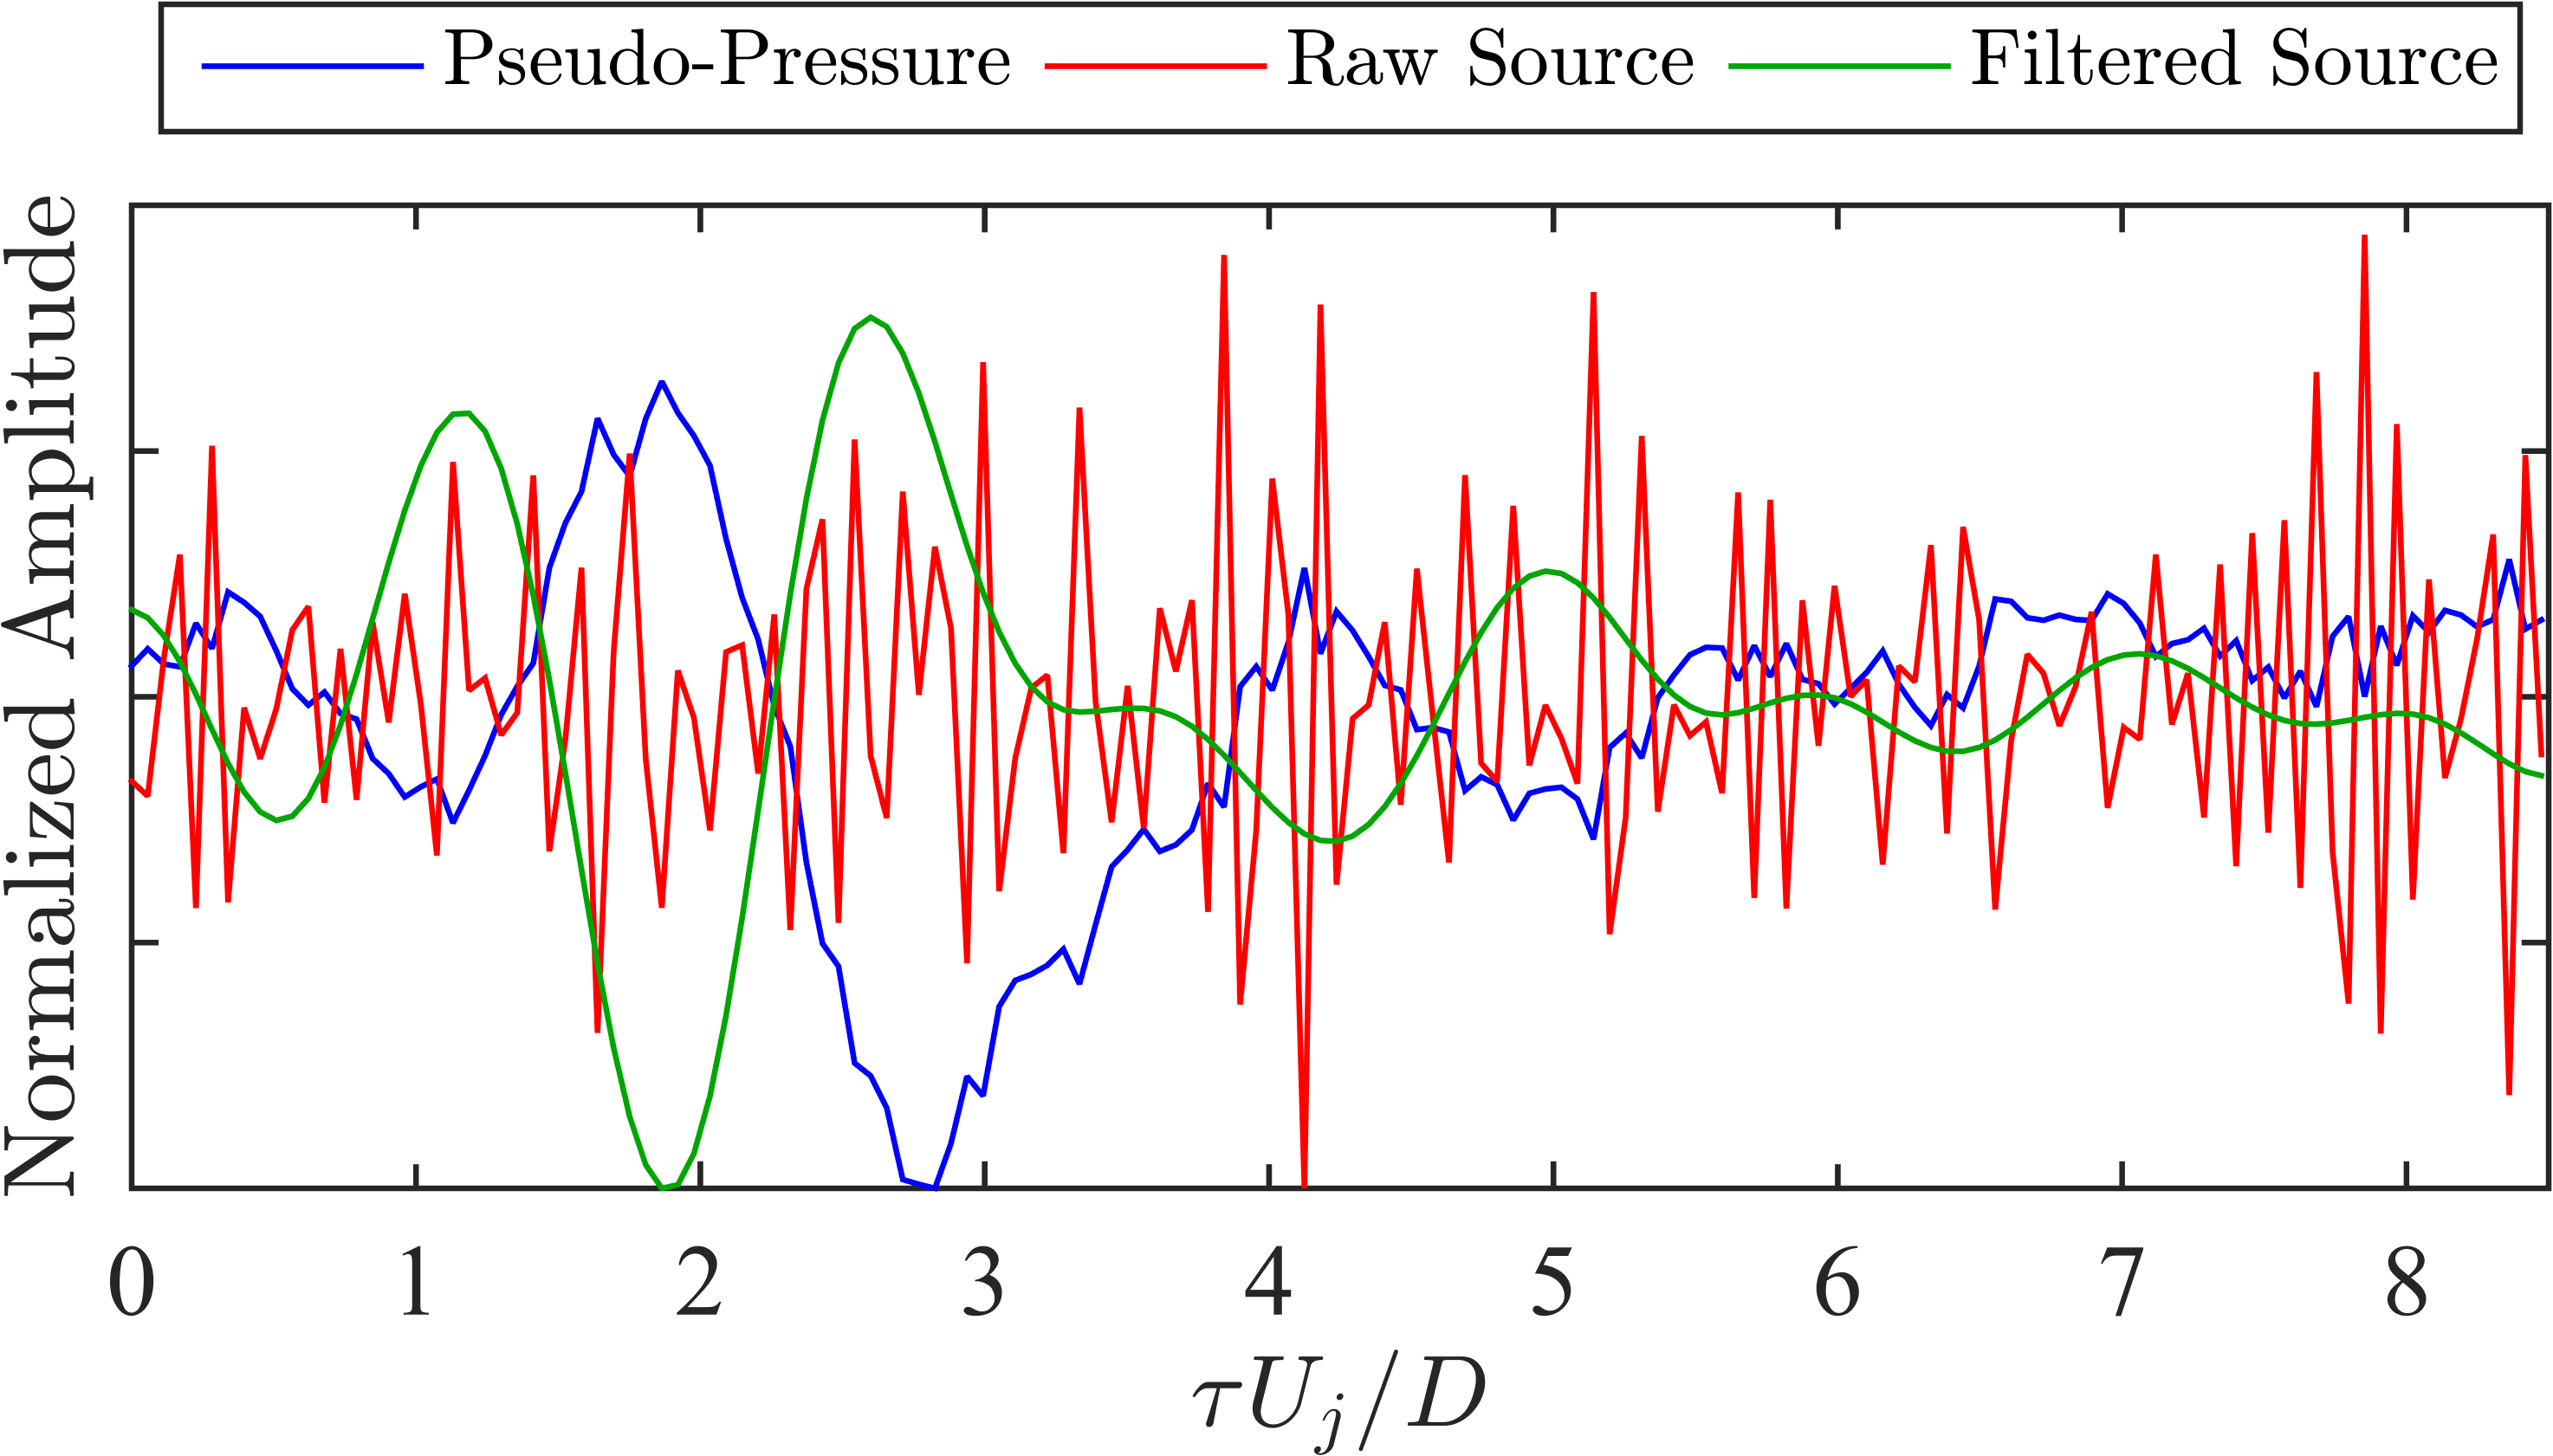
\includegraphics[width = 3.5in]{Figures/ch5_valid_denoising.png}
%	\caption{Effects of filtering of the pseudo-pressure field on the calculated aeroacoustic source at $x/D = 1.75, r/D = 0.5$; amplitudes have been arbitrarily normalized to ease visual comparisons.}
%	\label{fig:valid_denoising}
%\end{figure}
%
%Once the pseudo-pressure field has been properly filtered, the aeroacoustic source is simply calculated using second-order finite differences in time (\fig{fig:valid_denoising}).
%To compute the far-field noise, the source field can be spatially-integrated in retarded time, accounting for the propagation delay from each source location to the observer, per \eq{eq:source_integration}; here, this was performed by trapezoidal integration. 
%\begin{figure}
%	\centering
%	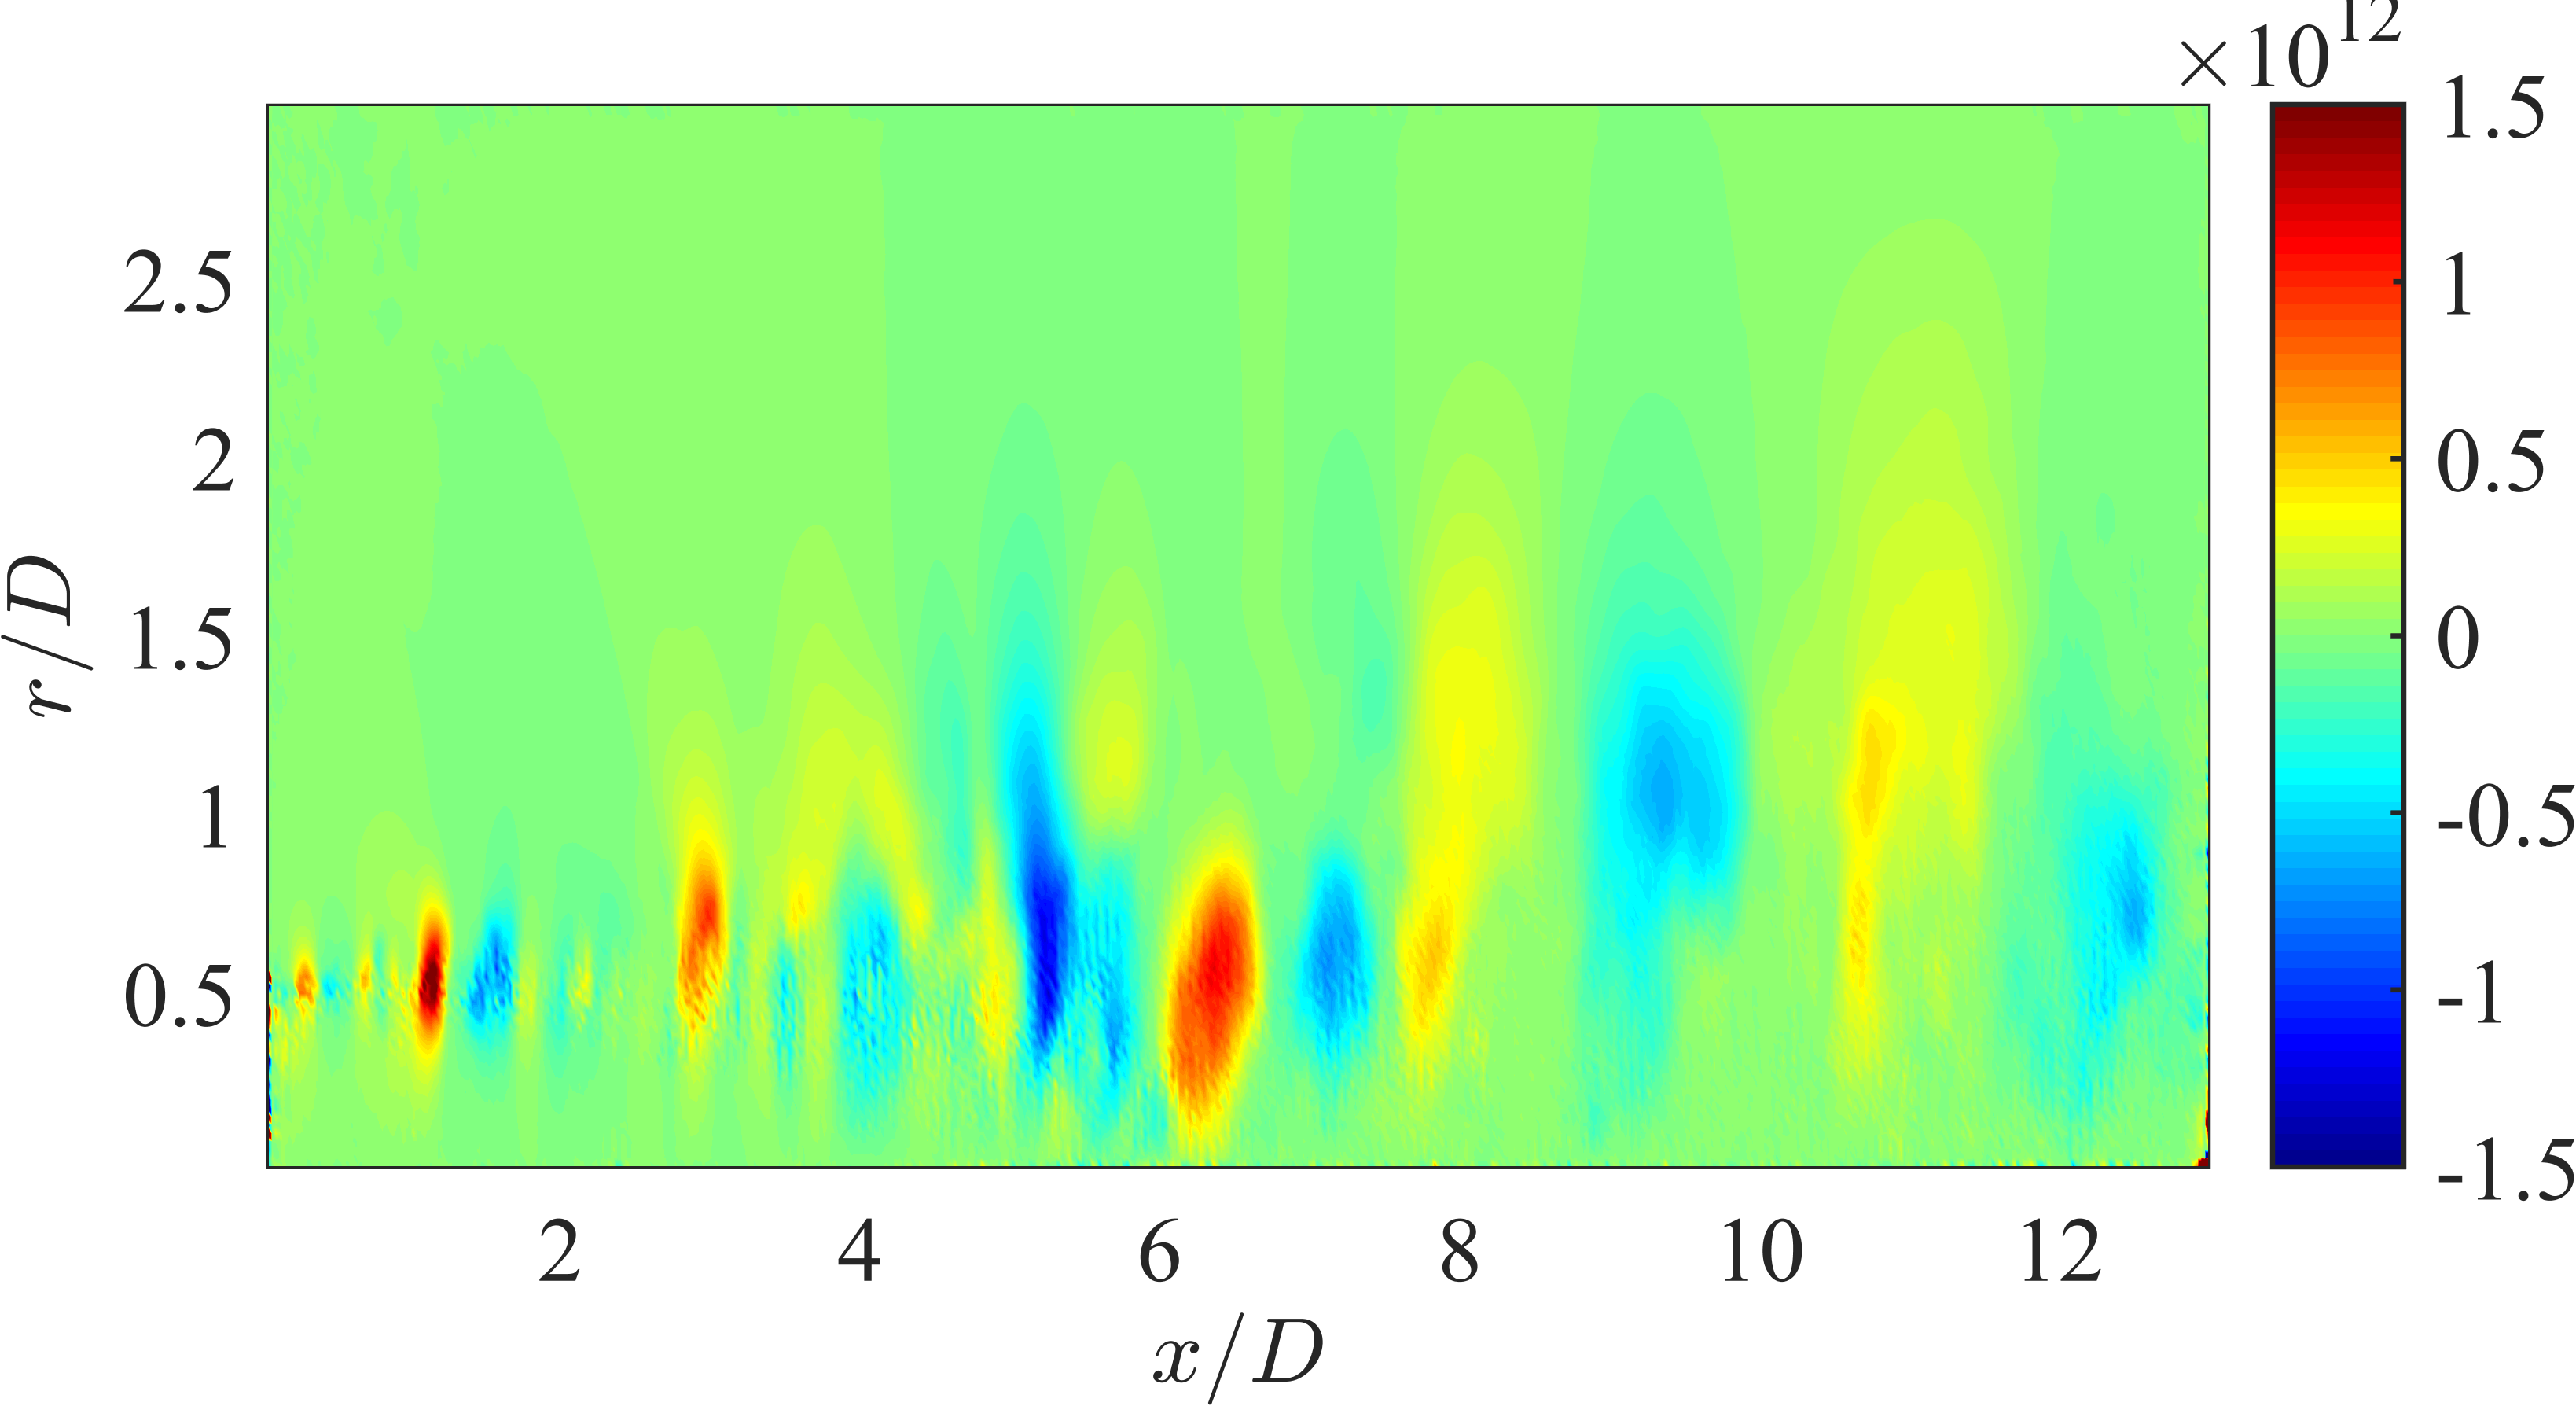
\includegraphics[width = 3.5in]{Figures/ch5_valid_Inst_source.png}
%	\caption{Instantaneous source field for the same conditions as \fig{fig:valid_helmholtz}.}
%	\label{fig:valid_source}
%\end{figure}
%
%\section{Wavepackets in the Pseudo-Pressure Field}
%The signature of the large-scale structures in the irrotational near-field pressure has been well-known for some time.
%As discussed in \sect{sect:nearfield}, the near-field pressure response to a large-scale structure takes the form of a compact wave which is modulated in amplitude and spatial extent as it convects through the jet shear layer; the near-field response to excitation-induced large-scale structures is discussed in more detail by Sinha \etal \citep{Sinha2012}.
%Similar results have also been found by Tinney \& Jordan \citep{Tinney2008} in a natural, subsonic jet.
%Per Ribner's analysis, these near-field pressure signatures are related to the noise sources and hence can serve as a useful validation of the computed pseudo-pressure fields since they are close physical analogues (though the hydrodynamic component of the irrotational near-field pressure isn't strictly incompressible, compressibility effects are minor). 
%\begin{figure}
%	\centering
%	\begin{subfigure}{.5\textwidth}
%		\centering
%		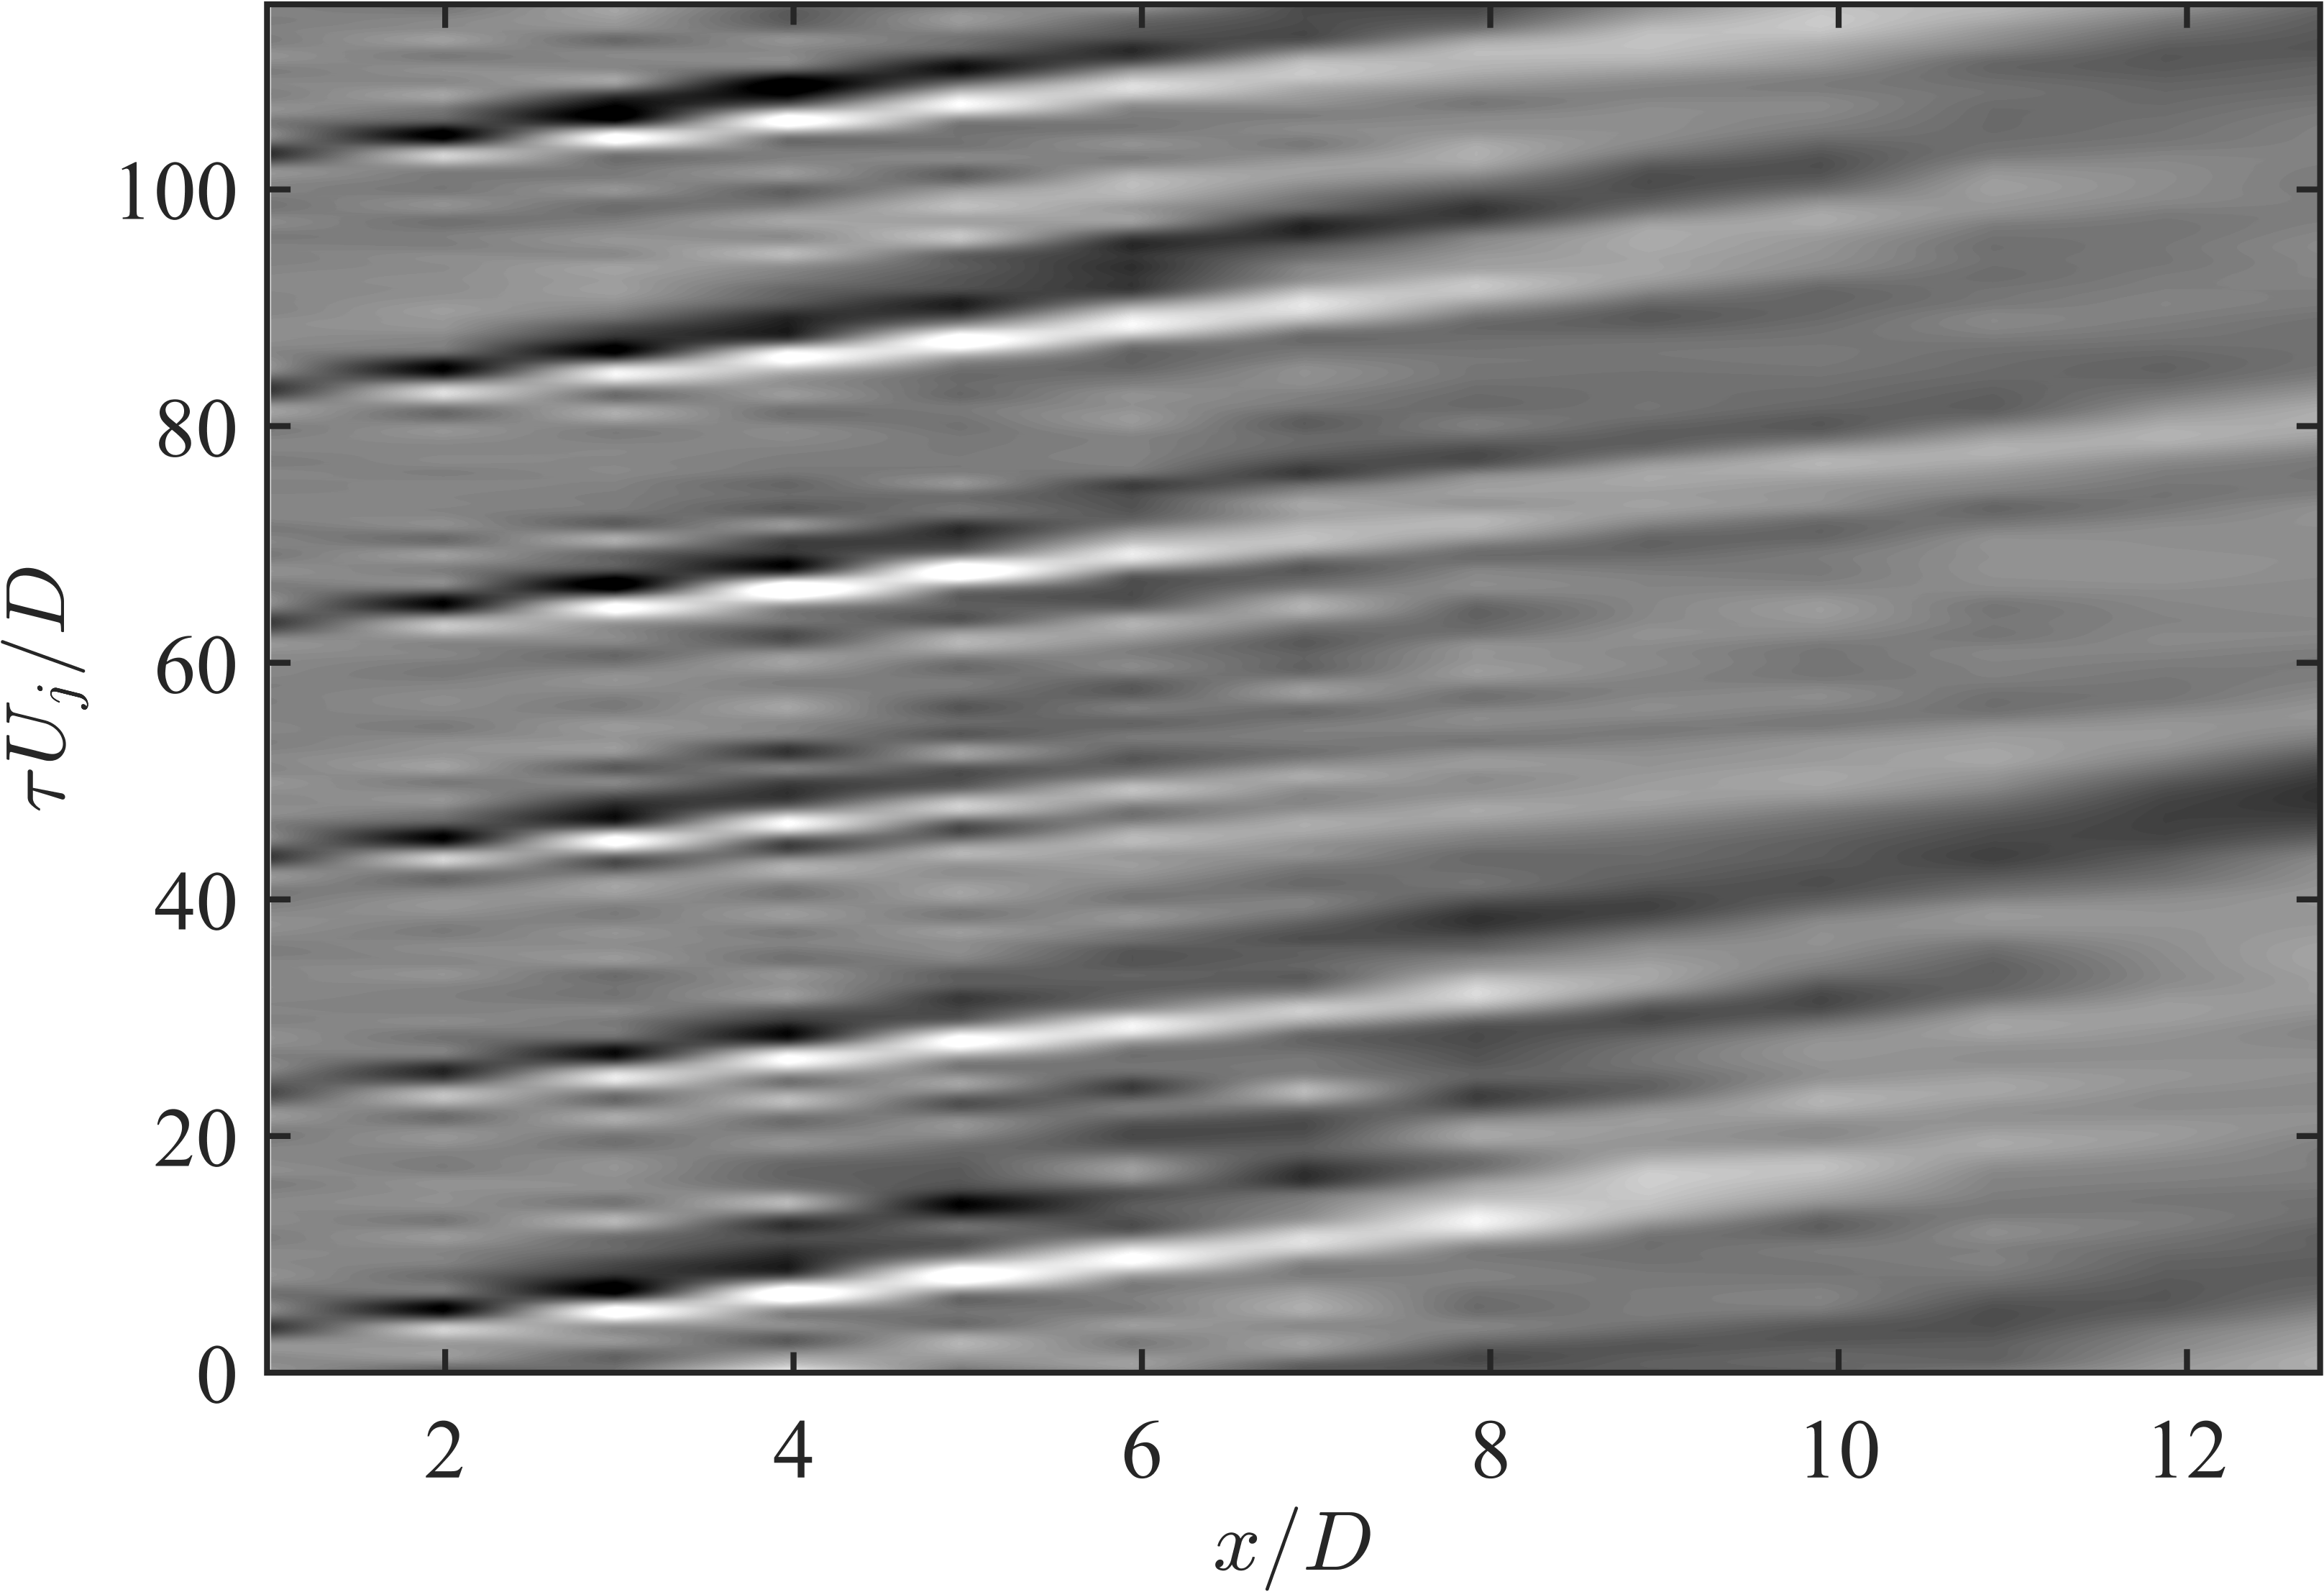
\includegraphics[width=0.95\linewidth]{Figures/ch5_st005_NearField_wvpkts.png}
%		\caption{}
%	\end{subfigure}%
%	\begin{subfigure}{.5\textwidth}
%		\centering
%		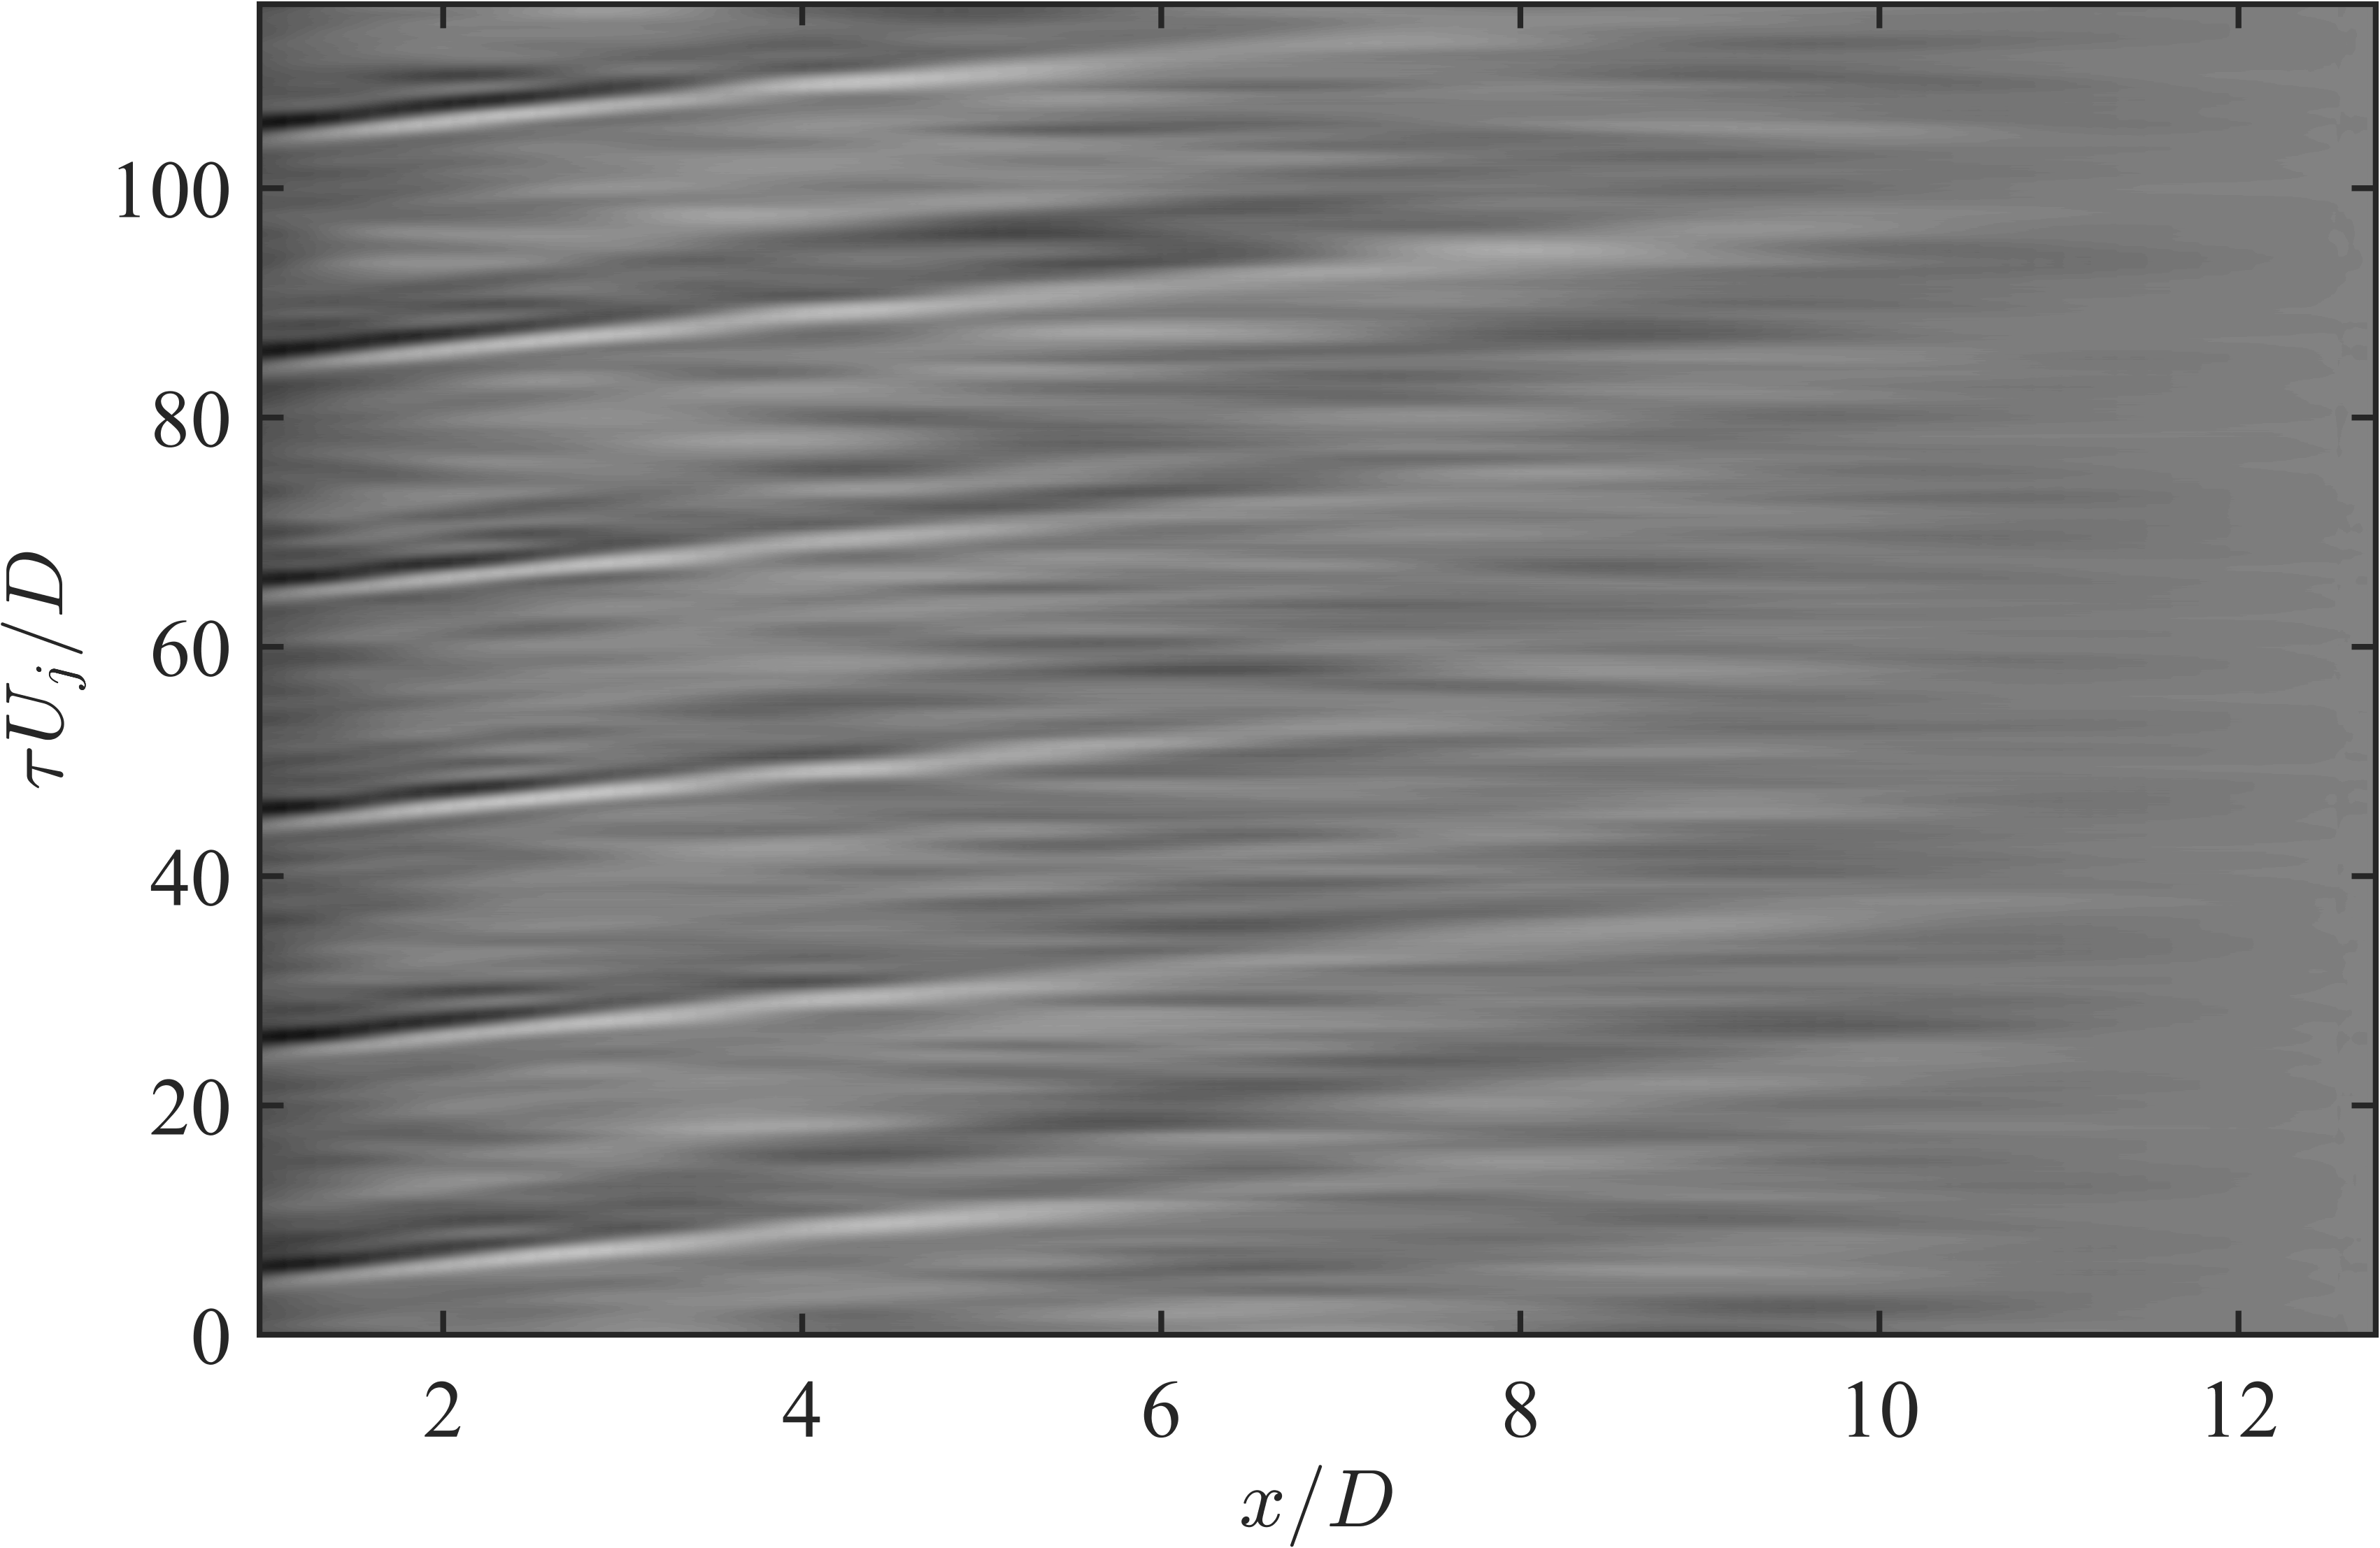
\includegraphics[width=0.95\linewidth]{Figures/ch5_st005_FlowField_wvpkts.png}
%		\caption{}
%	\end{subfigure}\\
%	\begin{subfigure}{.5\textwidth}
%		\centering
%		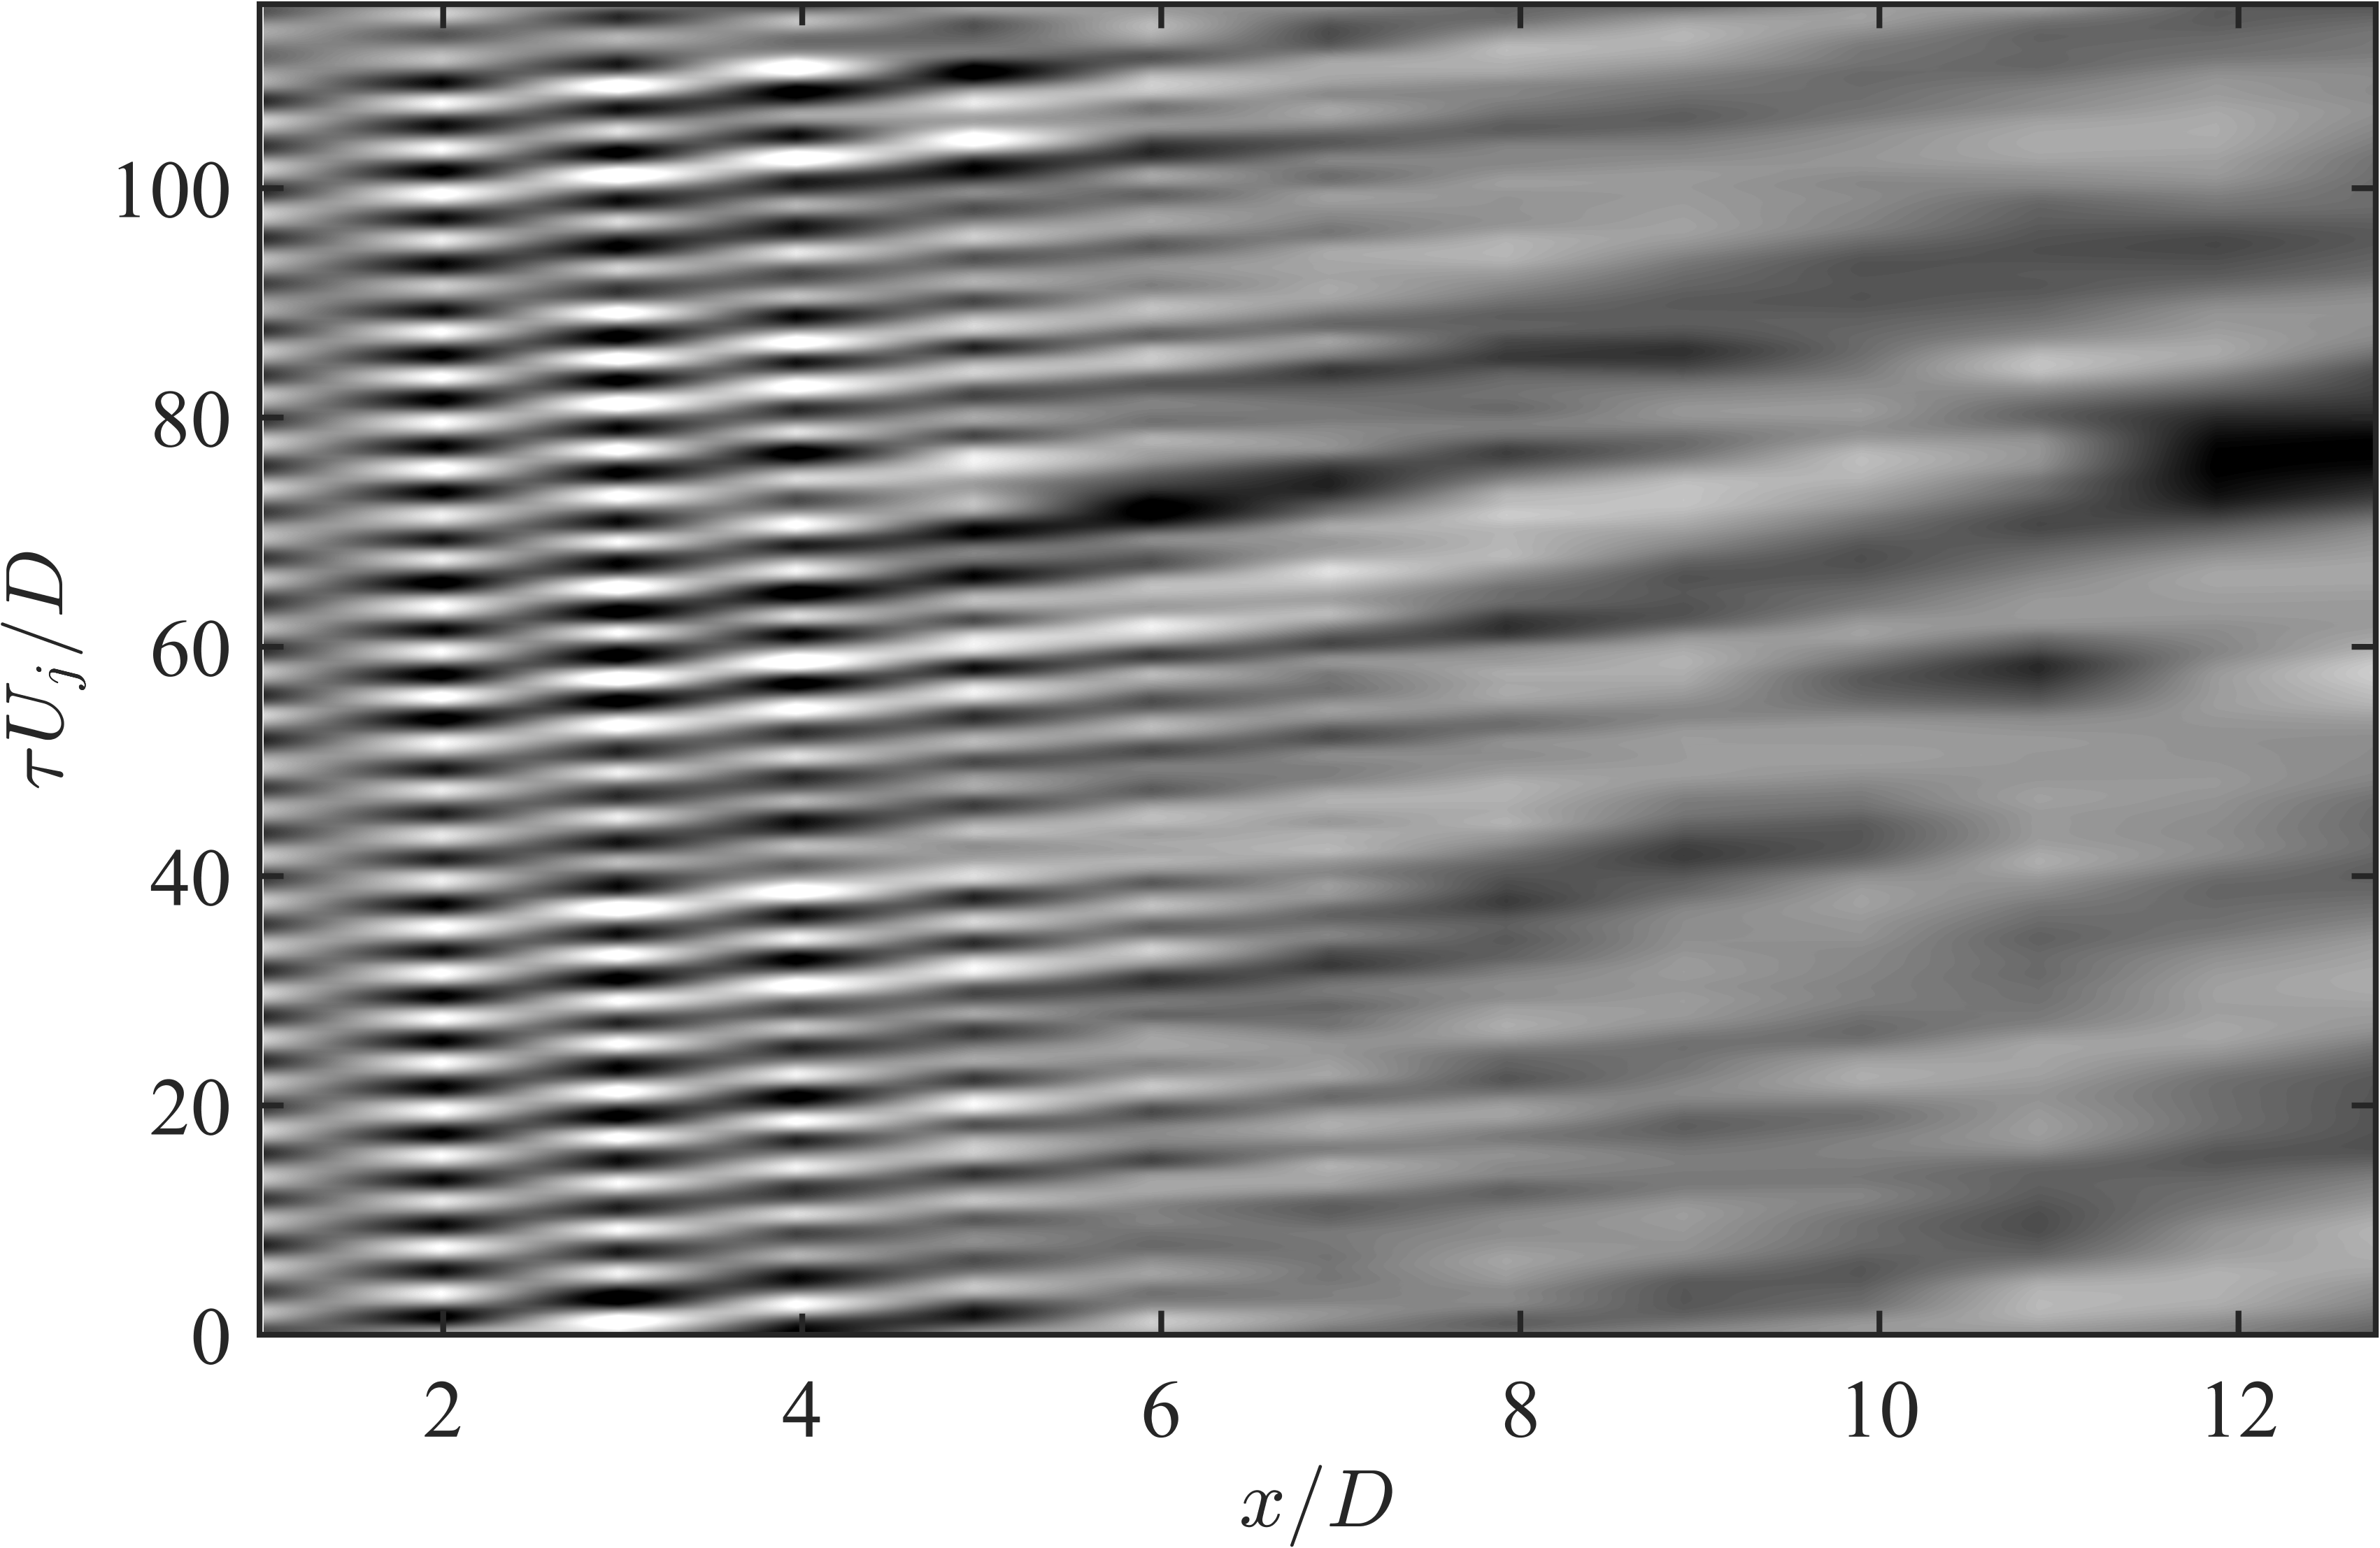
\includegraphics[width=0.95\linewidth]{Figures/ch5_st025_NearField_wvpkts.png}
%		\caption{}
%	\end{subfigure}%
%	\begin{subfigure}{.5\textwidth}
%		\centering
%		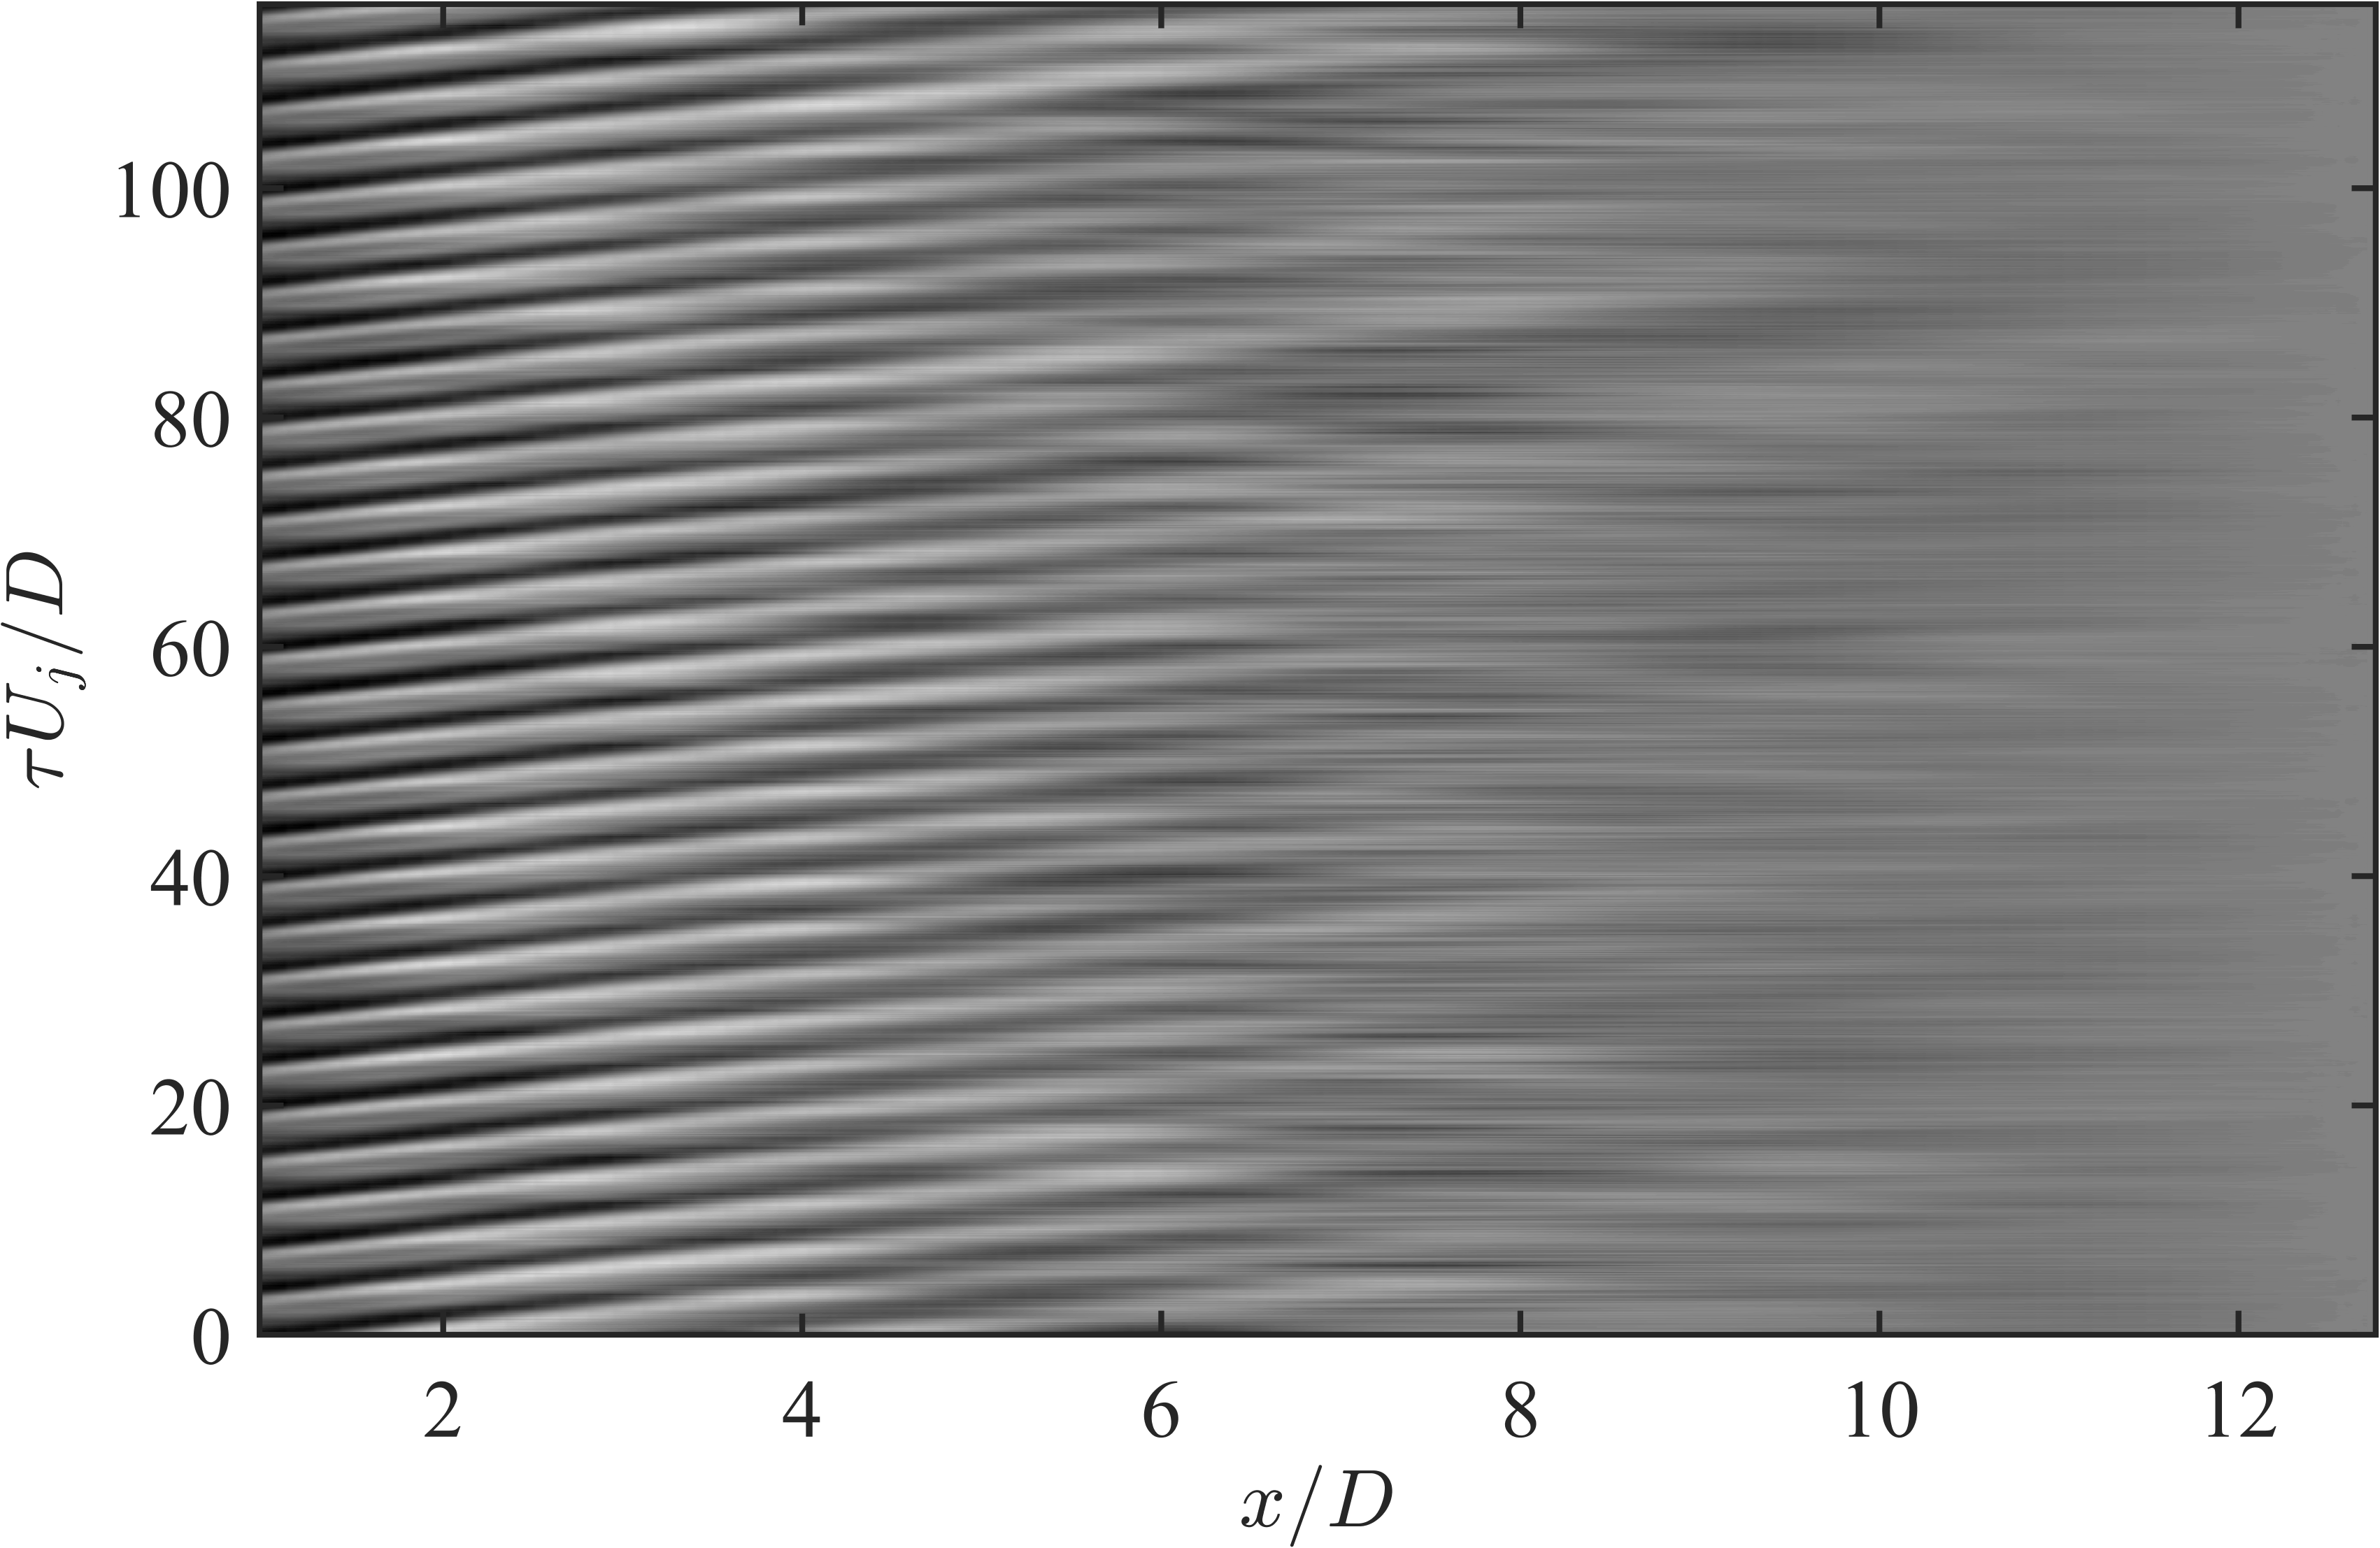
\includegraphics[width=0.95\linewidth]{Figures/ch5_st025_FlowField_wvpkts.png}
%		\caption{}
%	\end{subfigure}
%	\caption{Comparison of wavepackets measured from the hydrodynamic component of the irrotational near-field (a,c) against those in the computed pseudo-pressure field (b,d) for $St_{DF} = 0.05$ (a,b) and $St_{DF} = 0.25$ (c,d). A constant intensity map of $\pm 500$ Pa was used for all plots, and the experimentally measured near-field pressure was acquired \textbf{separately} from the velocity fields used to compute the pseudo-pressure.}
%	\label{fig:flowfield_wvpkts}
%\end{figure}
%
%In \fig{fig:flowfield_wvpkts} the hydrodynamic component of the irrotational near-field pressure as measured directly by the linear microphone array is compared against the pseudo-pressure field computed from the estimated time-resolved velocity fields for two excitation frequencies. 
%The `probe' locations in the pseudo-pressure field were chosen to mimic those of the near-field microphone array (just outside the shear layer and inclined $8.6^\circ$ with respect to the jet axis), just at a much higher spatial resolution.
%Note that the irrotational pressure fields shown were acquired separately, \ie near-field pressure measurements from the first experimental setup in \sect{sect:NF_methodology} are being compared against pseudo-pressure estimated using pressure measurements from the second experimental setup. 
%
%As expected, a clear wavepacket response is observed in the pseudo-pressure fields at the excitation frequency, similar to the behavior found in the hydrodynamic near-field pressure (note that the poor spatial resolution of the near-field microphones is producing an aliasing error for $St_{DF}=0.25$).
%For both fields and excitation frequencies, the wavepackets are the strongest and most coherent upstream of the end of the potential core.
%Downstream of the potential core, the flow is far more disorderly, as some of the LAFPA-induced structures have broken down completely while others have not - this is most readily observed for $St_{DF}=0.05$ where more than a few LAFPA-induced structures persist weakly far downstream.
%Surprisingly, the amplitude of the pseudo-pressure response is quite similar to that of the measured near-field pressure response (though by no means identical).
%
%The pseudo-pressure field does unfortunately exhibit a poor match against the measured near-field pressure in the far-downstream region; the cause for this is two-fold.
%First, since the pressure field is highly damped with radial distance and wavenumber \citep{Arndt1997}, estimating turbulent fluctuations near the jet centerline becomes increasingly difficult as the microphones move further away due to the spreading of the shear layer; the velocity information just simply isn't present in the near-field pressure fluctuations.
%Second, as the structures begin to breakdown near the end of the potential core, they lose their axisymmetry.
%This presents additional difficulties for the stochastic estimation, since the near-field microphones are offset azimuthally from the PIV laser sheet a vortex captured in the streamwise slice of the flow-field is not
%necessarily azimuthally-coherent (note the many asymmetric POD modes found in \fig{fig:ch4_St005_PODmodes} and \fig{fig:ch4_St025_PODmodes}) and hence may not be captured by the microphones (or vice versa).
%Given the results of \sect{sect:nearfield} as well as Hileman \etal \citep{Hileman2005}, which found the dominant source region to be located near the end of the potential core, rather than two potential core lengths downstream, this discrepancy between the measured and computed pressure fields, though unfortunate, is not expected to effect the final results or interpretation thereof.  
%
%\section{Accuracy of the Acoustic Far-field}
%As will be shown in the following section, the energy of the hydrodynamic field (pseudo-pressure) is orders of magnitude greater than the acoustic field.
%Hence, even slight experimental errors in the source field can overwhelm the computations for the acoustic field, rendering them next to meaningless for far-field predictions.
%This problem is not unique to Ribner's or Lighthill's approaches to the acoustic analogy; it plagues vortex sound theories as well \citep{Bridges1992}.
%In Ribner's dilatation acoustic analogy the source field takes the form of quadrupoles \citep{Ristorcelli1997}; the delicate interplay of these sources and sinks determining the acoustic far-field at a given spatial and temporal position.
%
%For reference, the computed acoustic signal at a far-field observer position matching the experimental far-field array ($R = 2.57$~m from the nozzle exit, at $\phi = 30^\circ$) has been plotted against the measured signal in \fig{fig:ch5_farfield}.
%For simplicity, the signals have been phase-averaged and only a single excitation period is shown.
%A coherent fluctuation could conceivably be observed in the acoustic field of the impulsively-excited jet (\fig{fig:ch5_farfield_imp}) centered around $\tau \simeq 0.8$, however given the lack of quiet time expected in the signal this could just as easily be wishful thinking.
%An offset in the time-of-arrival for the coherent wave between the calculated and measured signals could be due simply to an error in the positioning of the microphone relative to the nozzle exit, though given the poor match regardless of time-of-arrival, investigating this was deemed nonessential.
%Similarly, the computed acoustic signal for the periodic excitation cases ($St_{DF} = 0.25 \text{ and } 0.35$) bears only the vaguest similarities in shape and amplitude to the measured signal.
%Perhaps the most sympathetic observation of these plots is that the error between the measured and computed signals is at most $\sim 4$~Pa, or $\sim 0.1$\% of the peak amplitude of the pseudo-pressure field!
%Ultimately this means of course, that the computed source field should be viewed with some level of reservation, and hence will only be analyzed in the broadest of terms.
%\begin{figure}
%	\centering
%	\begin{subfigure}{1\textwidth}
%		\centering
%		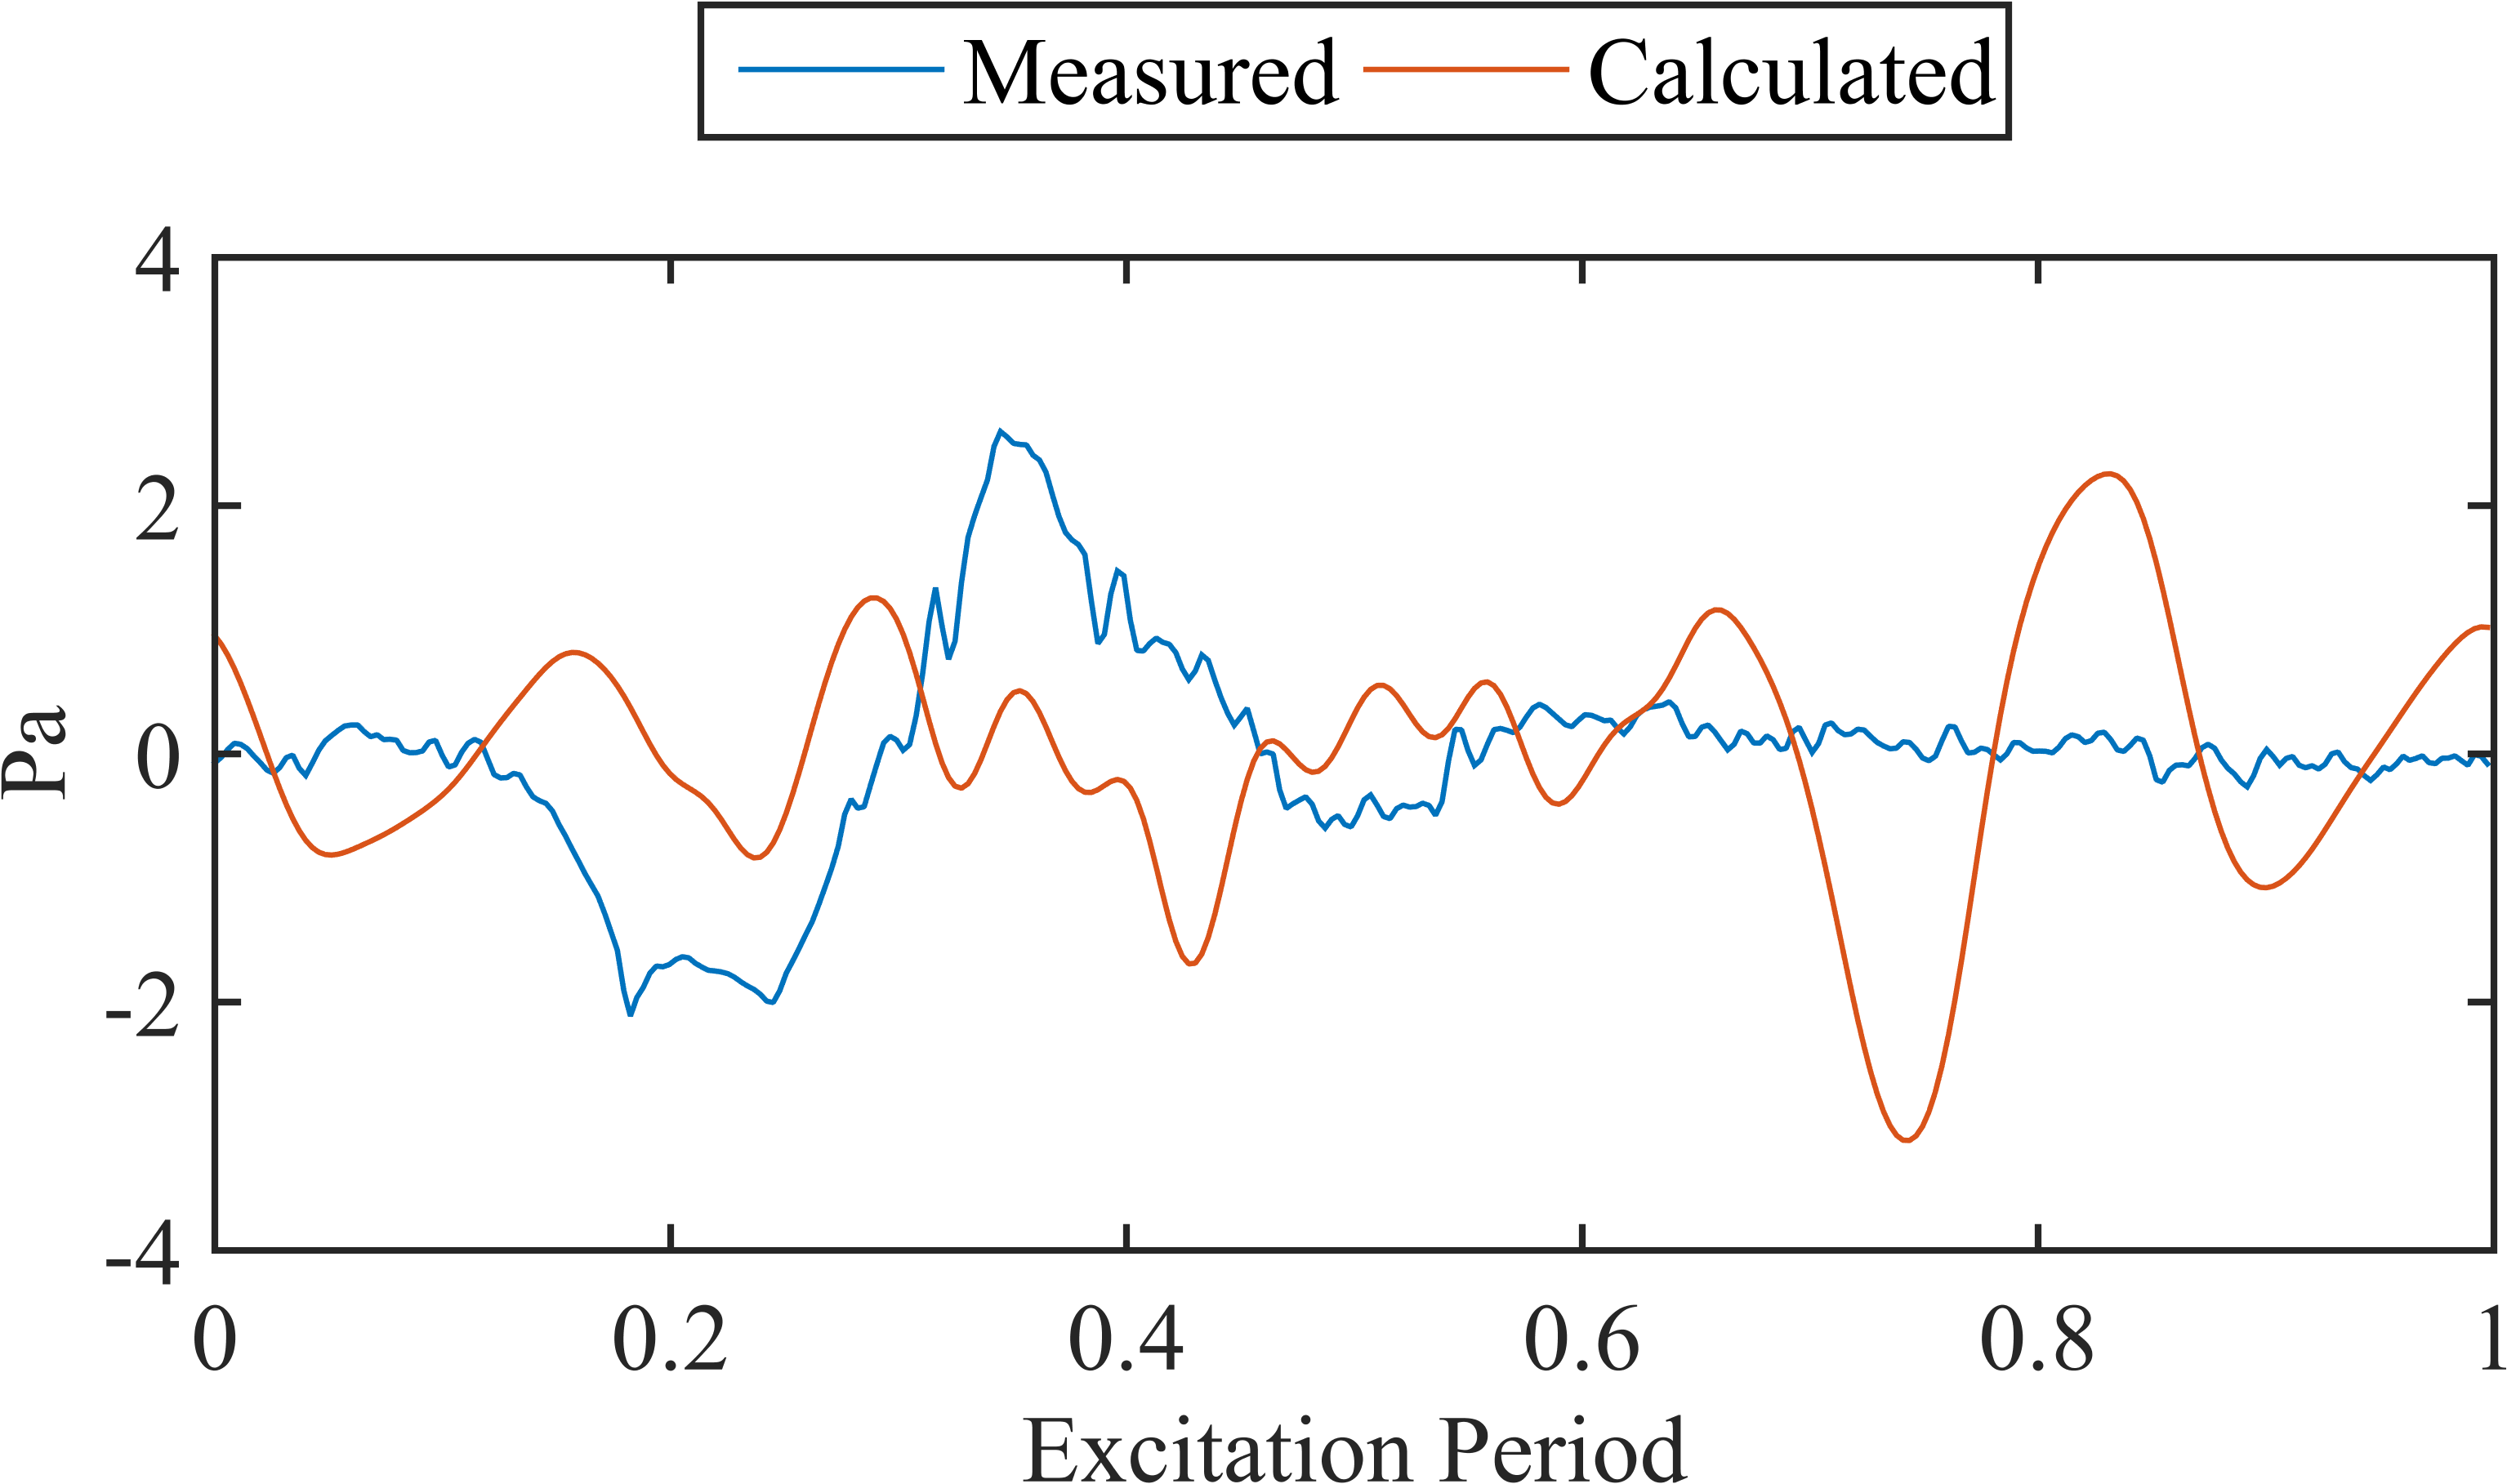
\includegraphics[width=3.5in]{Figures/ch5_St005_FF_v2.png}
%		\caption{$St_{DF} = 0.05$}
%		\label{fig:ch5_farfield_imp}
%	\end{subfigure}\\
%	\begin{subfigure}{1\textwidth}
%		\centering
%		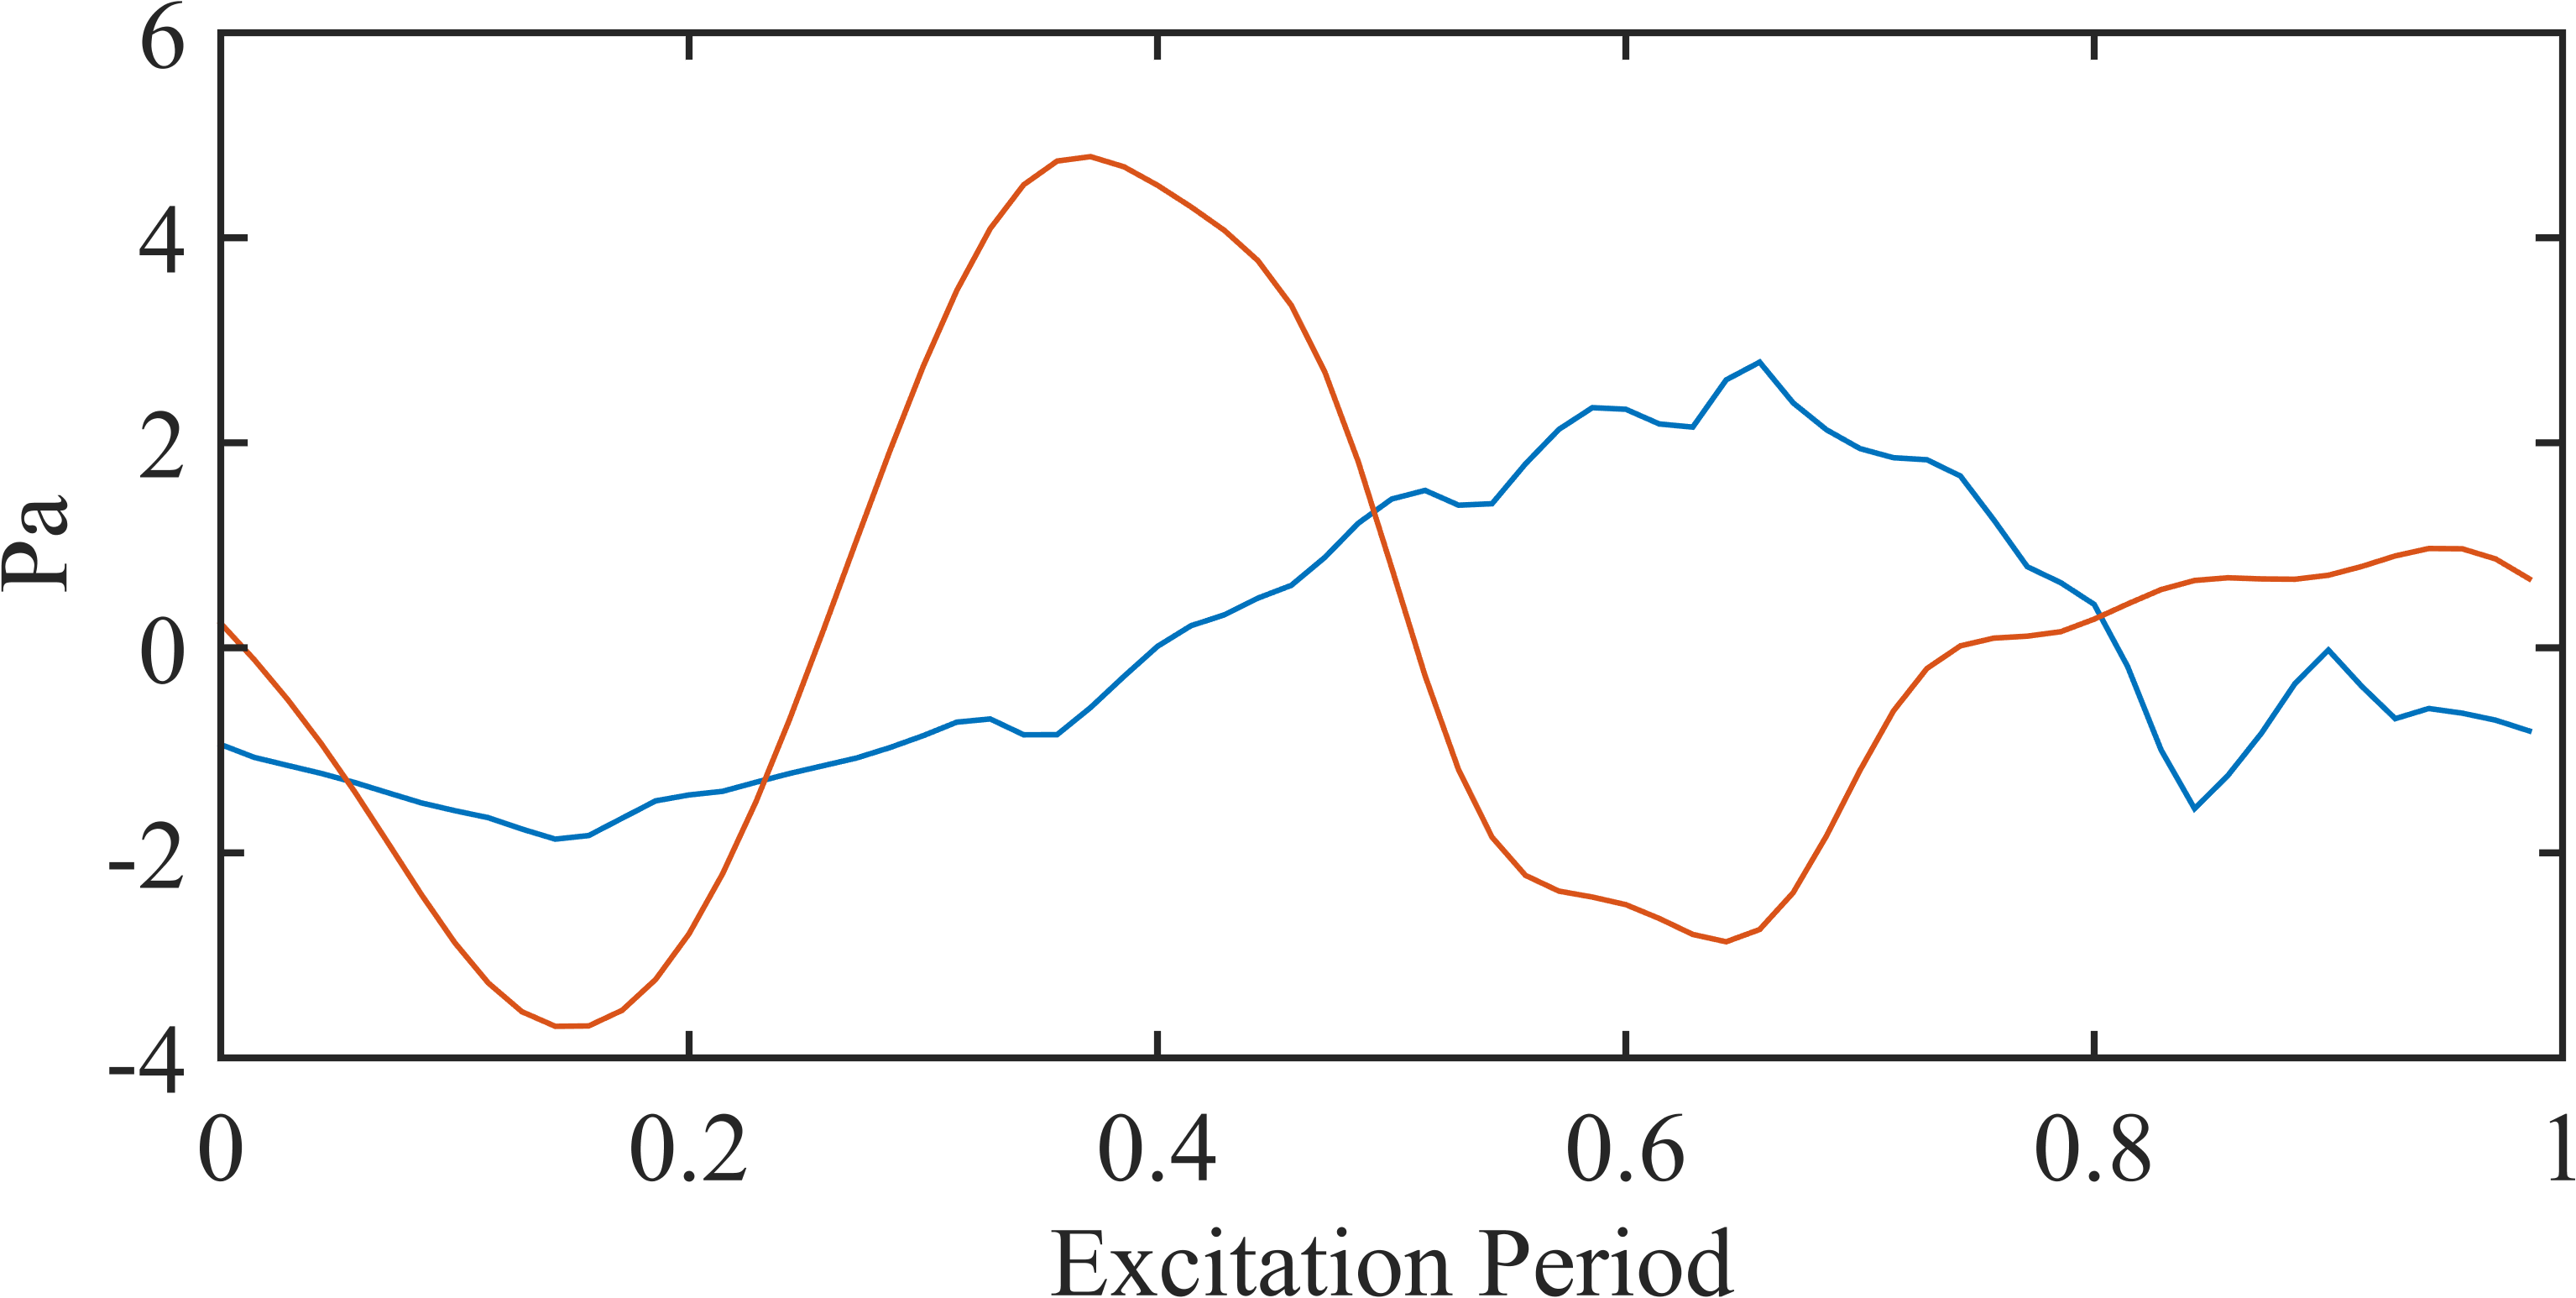
\includegraphics[width=3.5in]{Figures/ch5_St025_FF_v3.png}
%		\caption{$St_{DF} = 0.25$}
%	\end{subfigure}\\
%	\begin{subfigure}{1\textwidth}
%		\centering
%		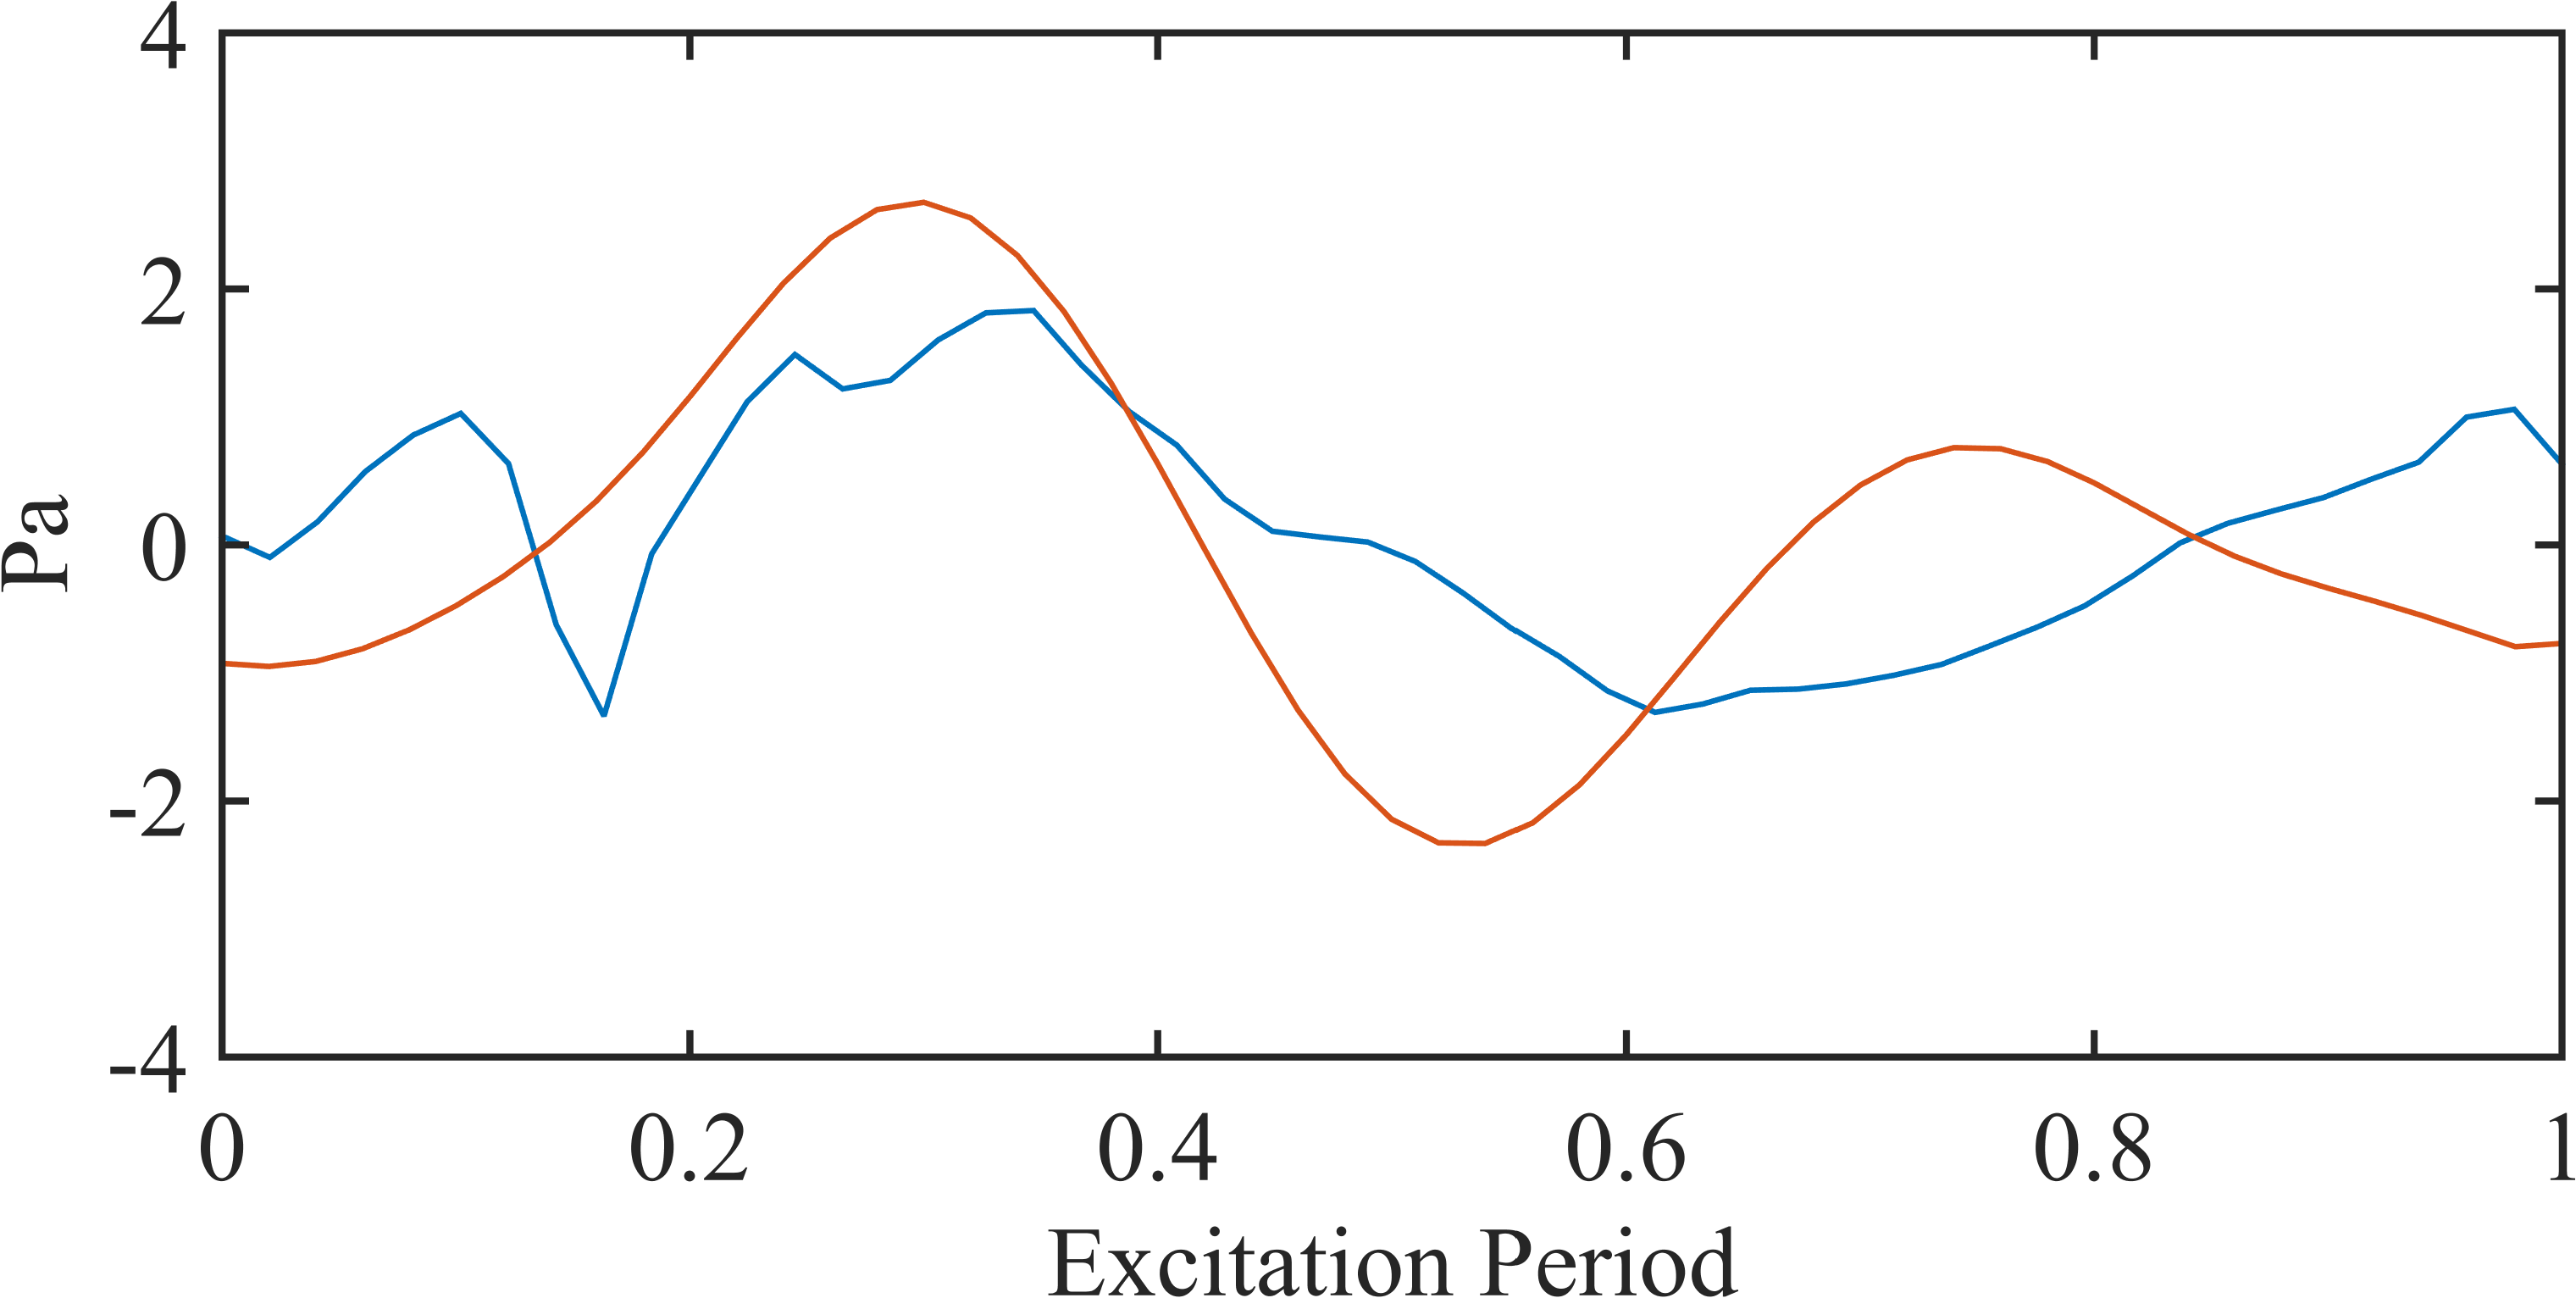
\includegraphics[width=3.5in]{Figures/ch5_St035_FF_v3.png}
%		\caption{$St_{DF} = 0.35$}
%	\end{subfigure}
%	\caption{Comparison of the phase-averaged far-field signal at $30^\circ$ computed from the source field against the signal measured by the far-field microphone array.}
%	\label{fig:ch5_farfield}
%\end{figure}
%
%\section{Aeroacoustic Behavior of Coherent Structures}
%The pseudo-pressure field induced by the coherent vortex takes the form of a spatially-modulated traveling wave; this can be observed in \fig{fig:PSL_St005}.
%A strong expansion wave is found to be centered on the vortex, preceded by an equally strong compression wave.
%As the vortex convects downstream and amplifies, the radial extent of the pressure fluctuation amplifies as well; initially the pressure fluctuation is concentrated only around the jet lipline but by $x/D \simeq 2$ the pressure fluctuations reach all the way to the jet centerline.
%These pressure fluctuations induce secondary, weaker fluctuations both precede and follow the dominant pair as they convect downstream.
%The strength of this traveling wave is directly proportional to the strength of the vortex, as the vortices begin to break down near $x/D = 4$, the pseudo-pressure fluctuations decay rapidly as well. 
%A similar behavior is observed for the periodically-excited jets ($St_{DF} = 0.25$ is shown in \fig{fig:PSL_St025}), though the pseudo-pressure field now of course takes the form of a periodic train of convecting vortices and modulating waves.
%Compared to the impulse-excitation case, the radial extent of the pressure fluctuations in the periodic-excitation cases grows much more rapidly.
%\begin{figure}
%	\centering
%	\begin{subfigure}{0.75\textwidth}
%		\centering
%		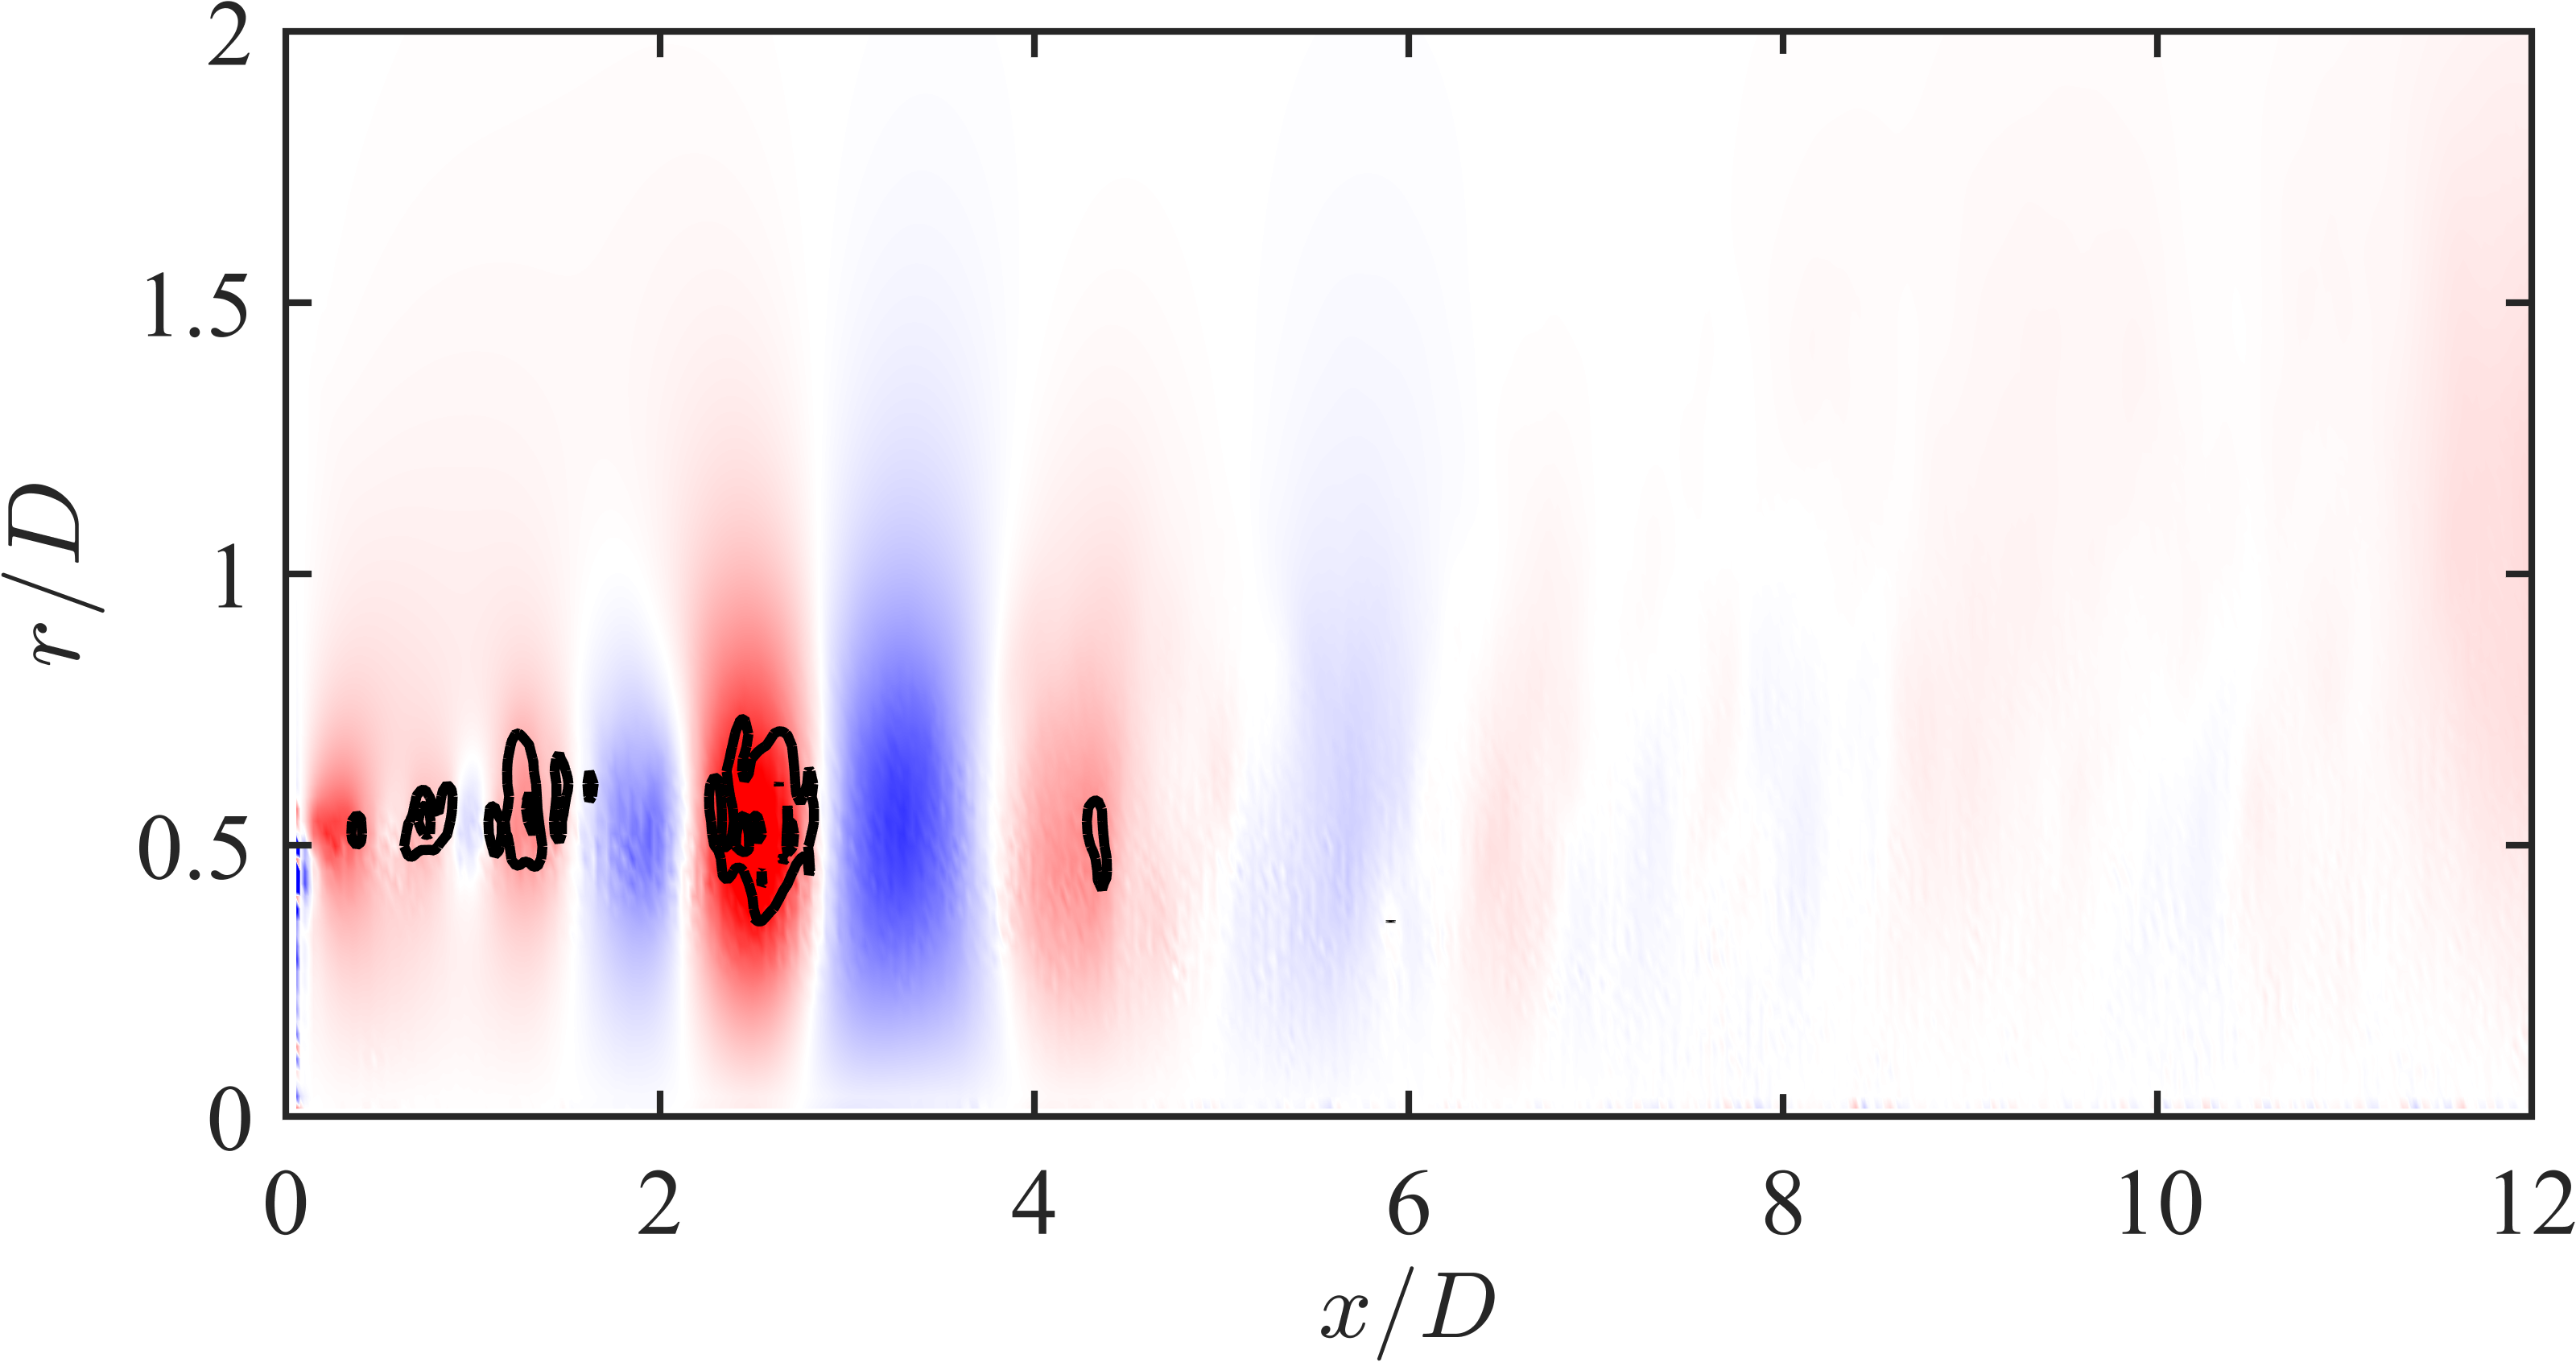
\includegraphics[width=0.95\linewidth]{Figures/ch5_St005_PSL_101.png}
%		\caption{$\phi = 9 \pi /16$}
%	\end{subfigure}\\
%	\begin{subfigure}{0.75\textwidth}
%		\centering
%		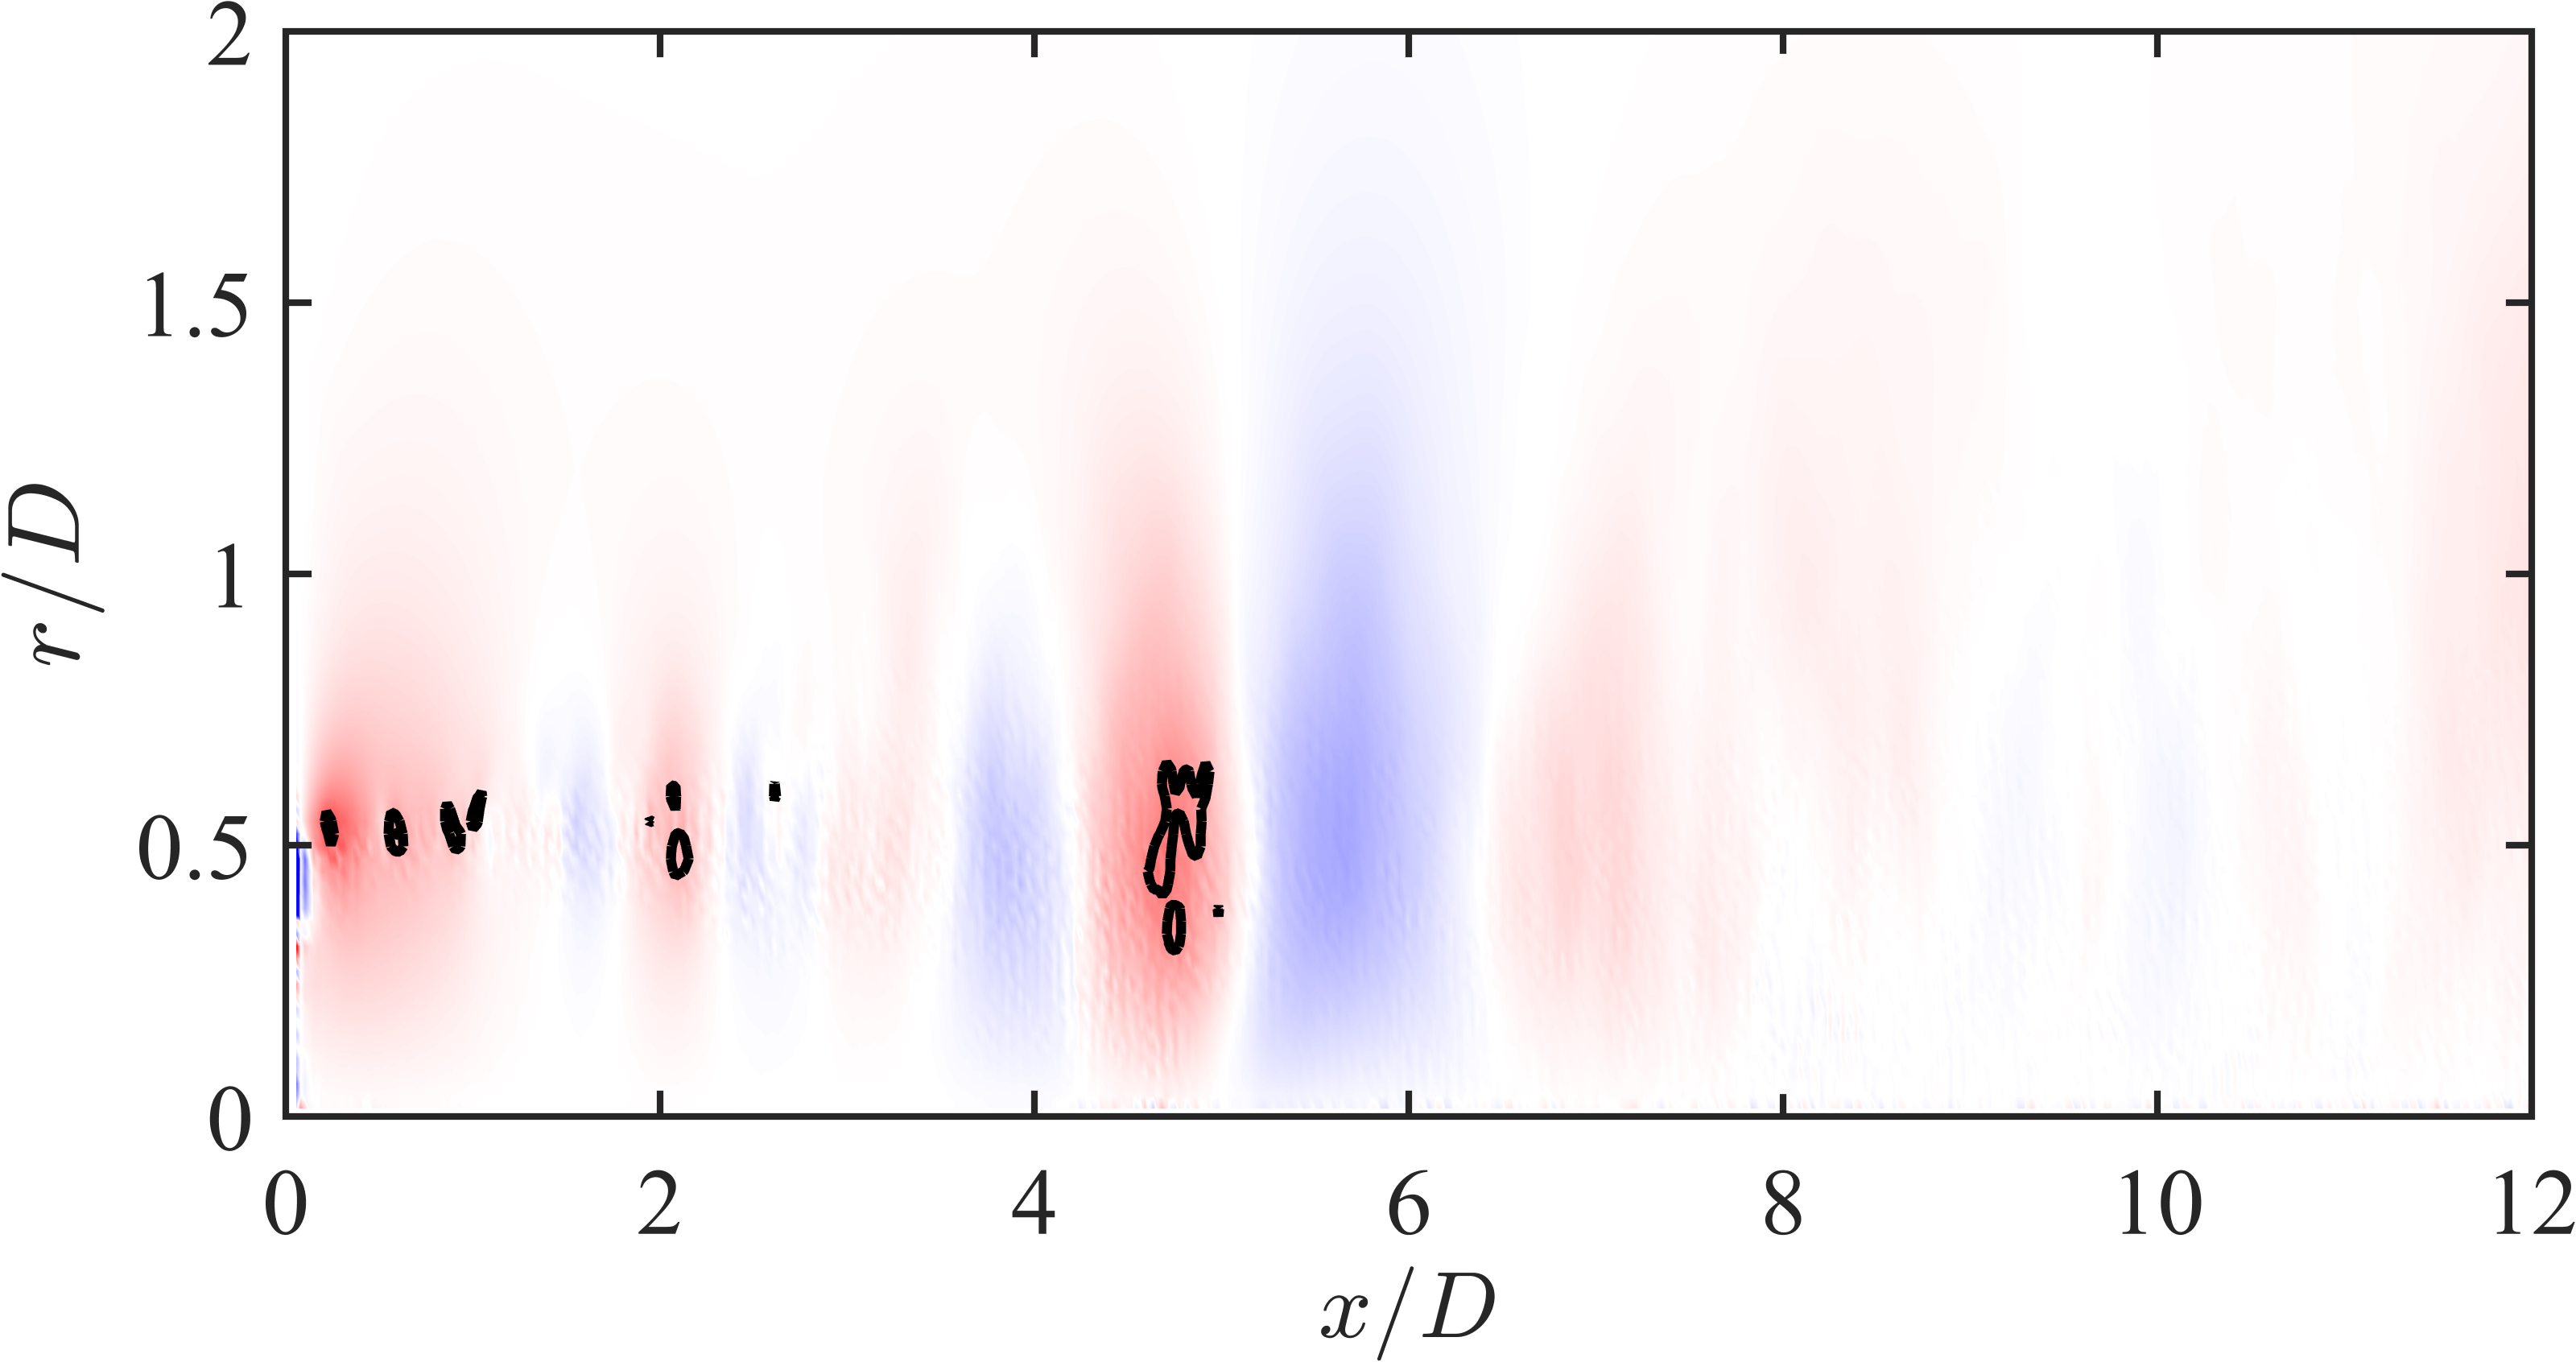
\includegraphics[width=0.95\linewidth]{Figures/ch5_St005_PSL_161.png}
%		\caption{$\phi = 7 \pi /8$}
%	\end{subfigure}
%	\caption{Pseudo-pressure field induced by the large-scale structure ($St_{DF} = 0.05$) at two excitation instances, with swirling strength overlain in black contours. A consistent color map (of $\pm 4000$~Pa) and contour level are used for the two plots; regions of red indicate negative fluctuations.}
%	\label{fig:PSL_St005}
%\end{figure}
%\begin{figure}
%	\centering
%	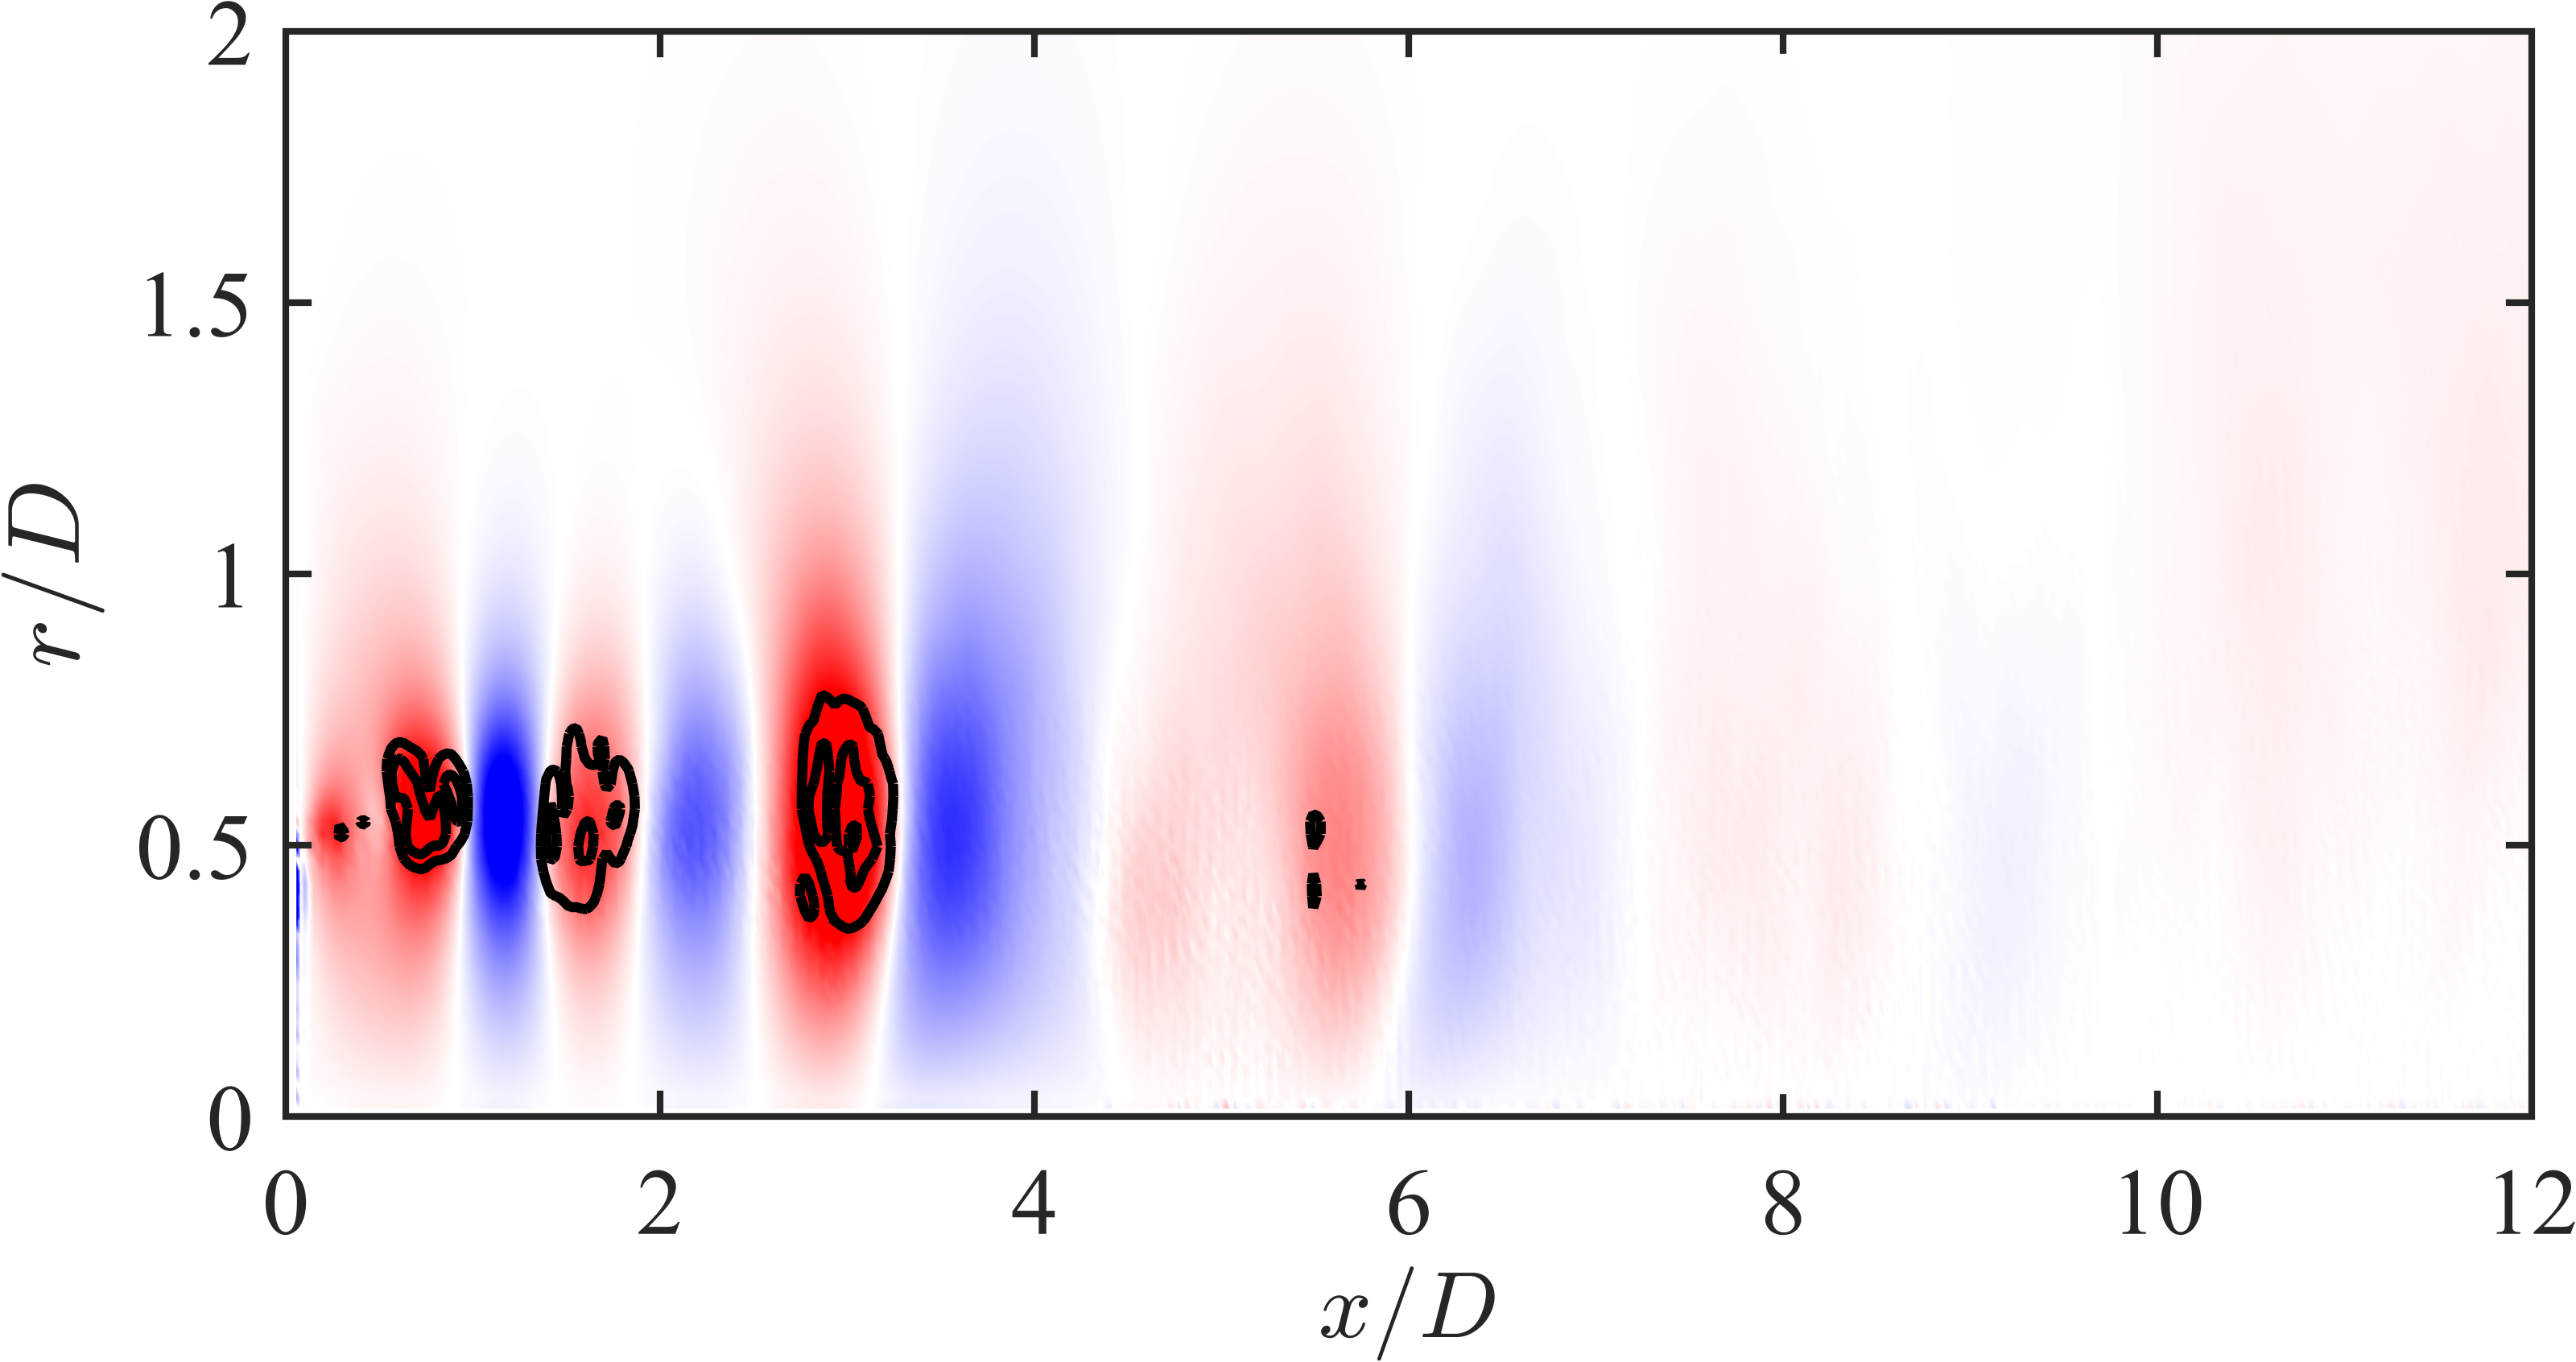
\includegraphics[width=0.70\linewidth]{Figures/ch5_St025_PSL_41.png}
%	\caption{Pseudo-pressure field induced by the periodic large-scale structures ($St_{DF} = 0.25$) at an arbitrary phase.}
%	\label{fig:PSL_St025}
%\end{figure}
%
%It should come as no surprise then that the aeroacoustic source would take the form of a wavepacket, centered around the coherent vortex.
%This is shown in \fig{fig:SL} for both the impulsively- and periodically-excited structures.
%Owing to the rapid growth and pairing process, the source field for the periodically-excited structures quickly amplifies and saturates by $x/D \simeq 2$.
%In contrast, a slow amplification is observed for the impulsive structure, which reaches its maximum amplitude just before the vortex begins to decay. 
%Based on the temporal extent of the acoustic response in the far-field, the acoustic wavelength of the emission produced by the individual ring vortex is $\sim 11D$, which would mean that the sources are non-compact per the results of \fig{fig:SL_St005}.
%This is in general agreement with the analysis of Michalke \citep{Michalke1972}, which showed that the experimentally observed far-field spectral directivity could be reproduced using an axially-coherent, noncompact source model.
%Of course, the amplitude of the source term alone does not determine acoustic emission; the acoustic emission is essentially the linear summation of the source/sink pairs (evaluated at retarded time) generated by the evolution of the vortices - a high amplitude source field coexisting with zero acoustic emission at a particular instant in time is therefore possible.
%A rapid truncation of the source term therefore has the potential to significantly amplify the acoustic emission.
%\begin{figure}
%	\centering
%	\begin{subfigure}{0.75\textwidth}
%		\centering
%		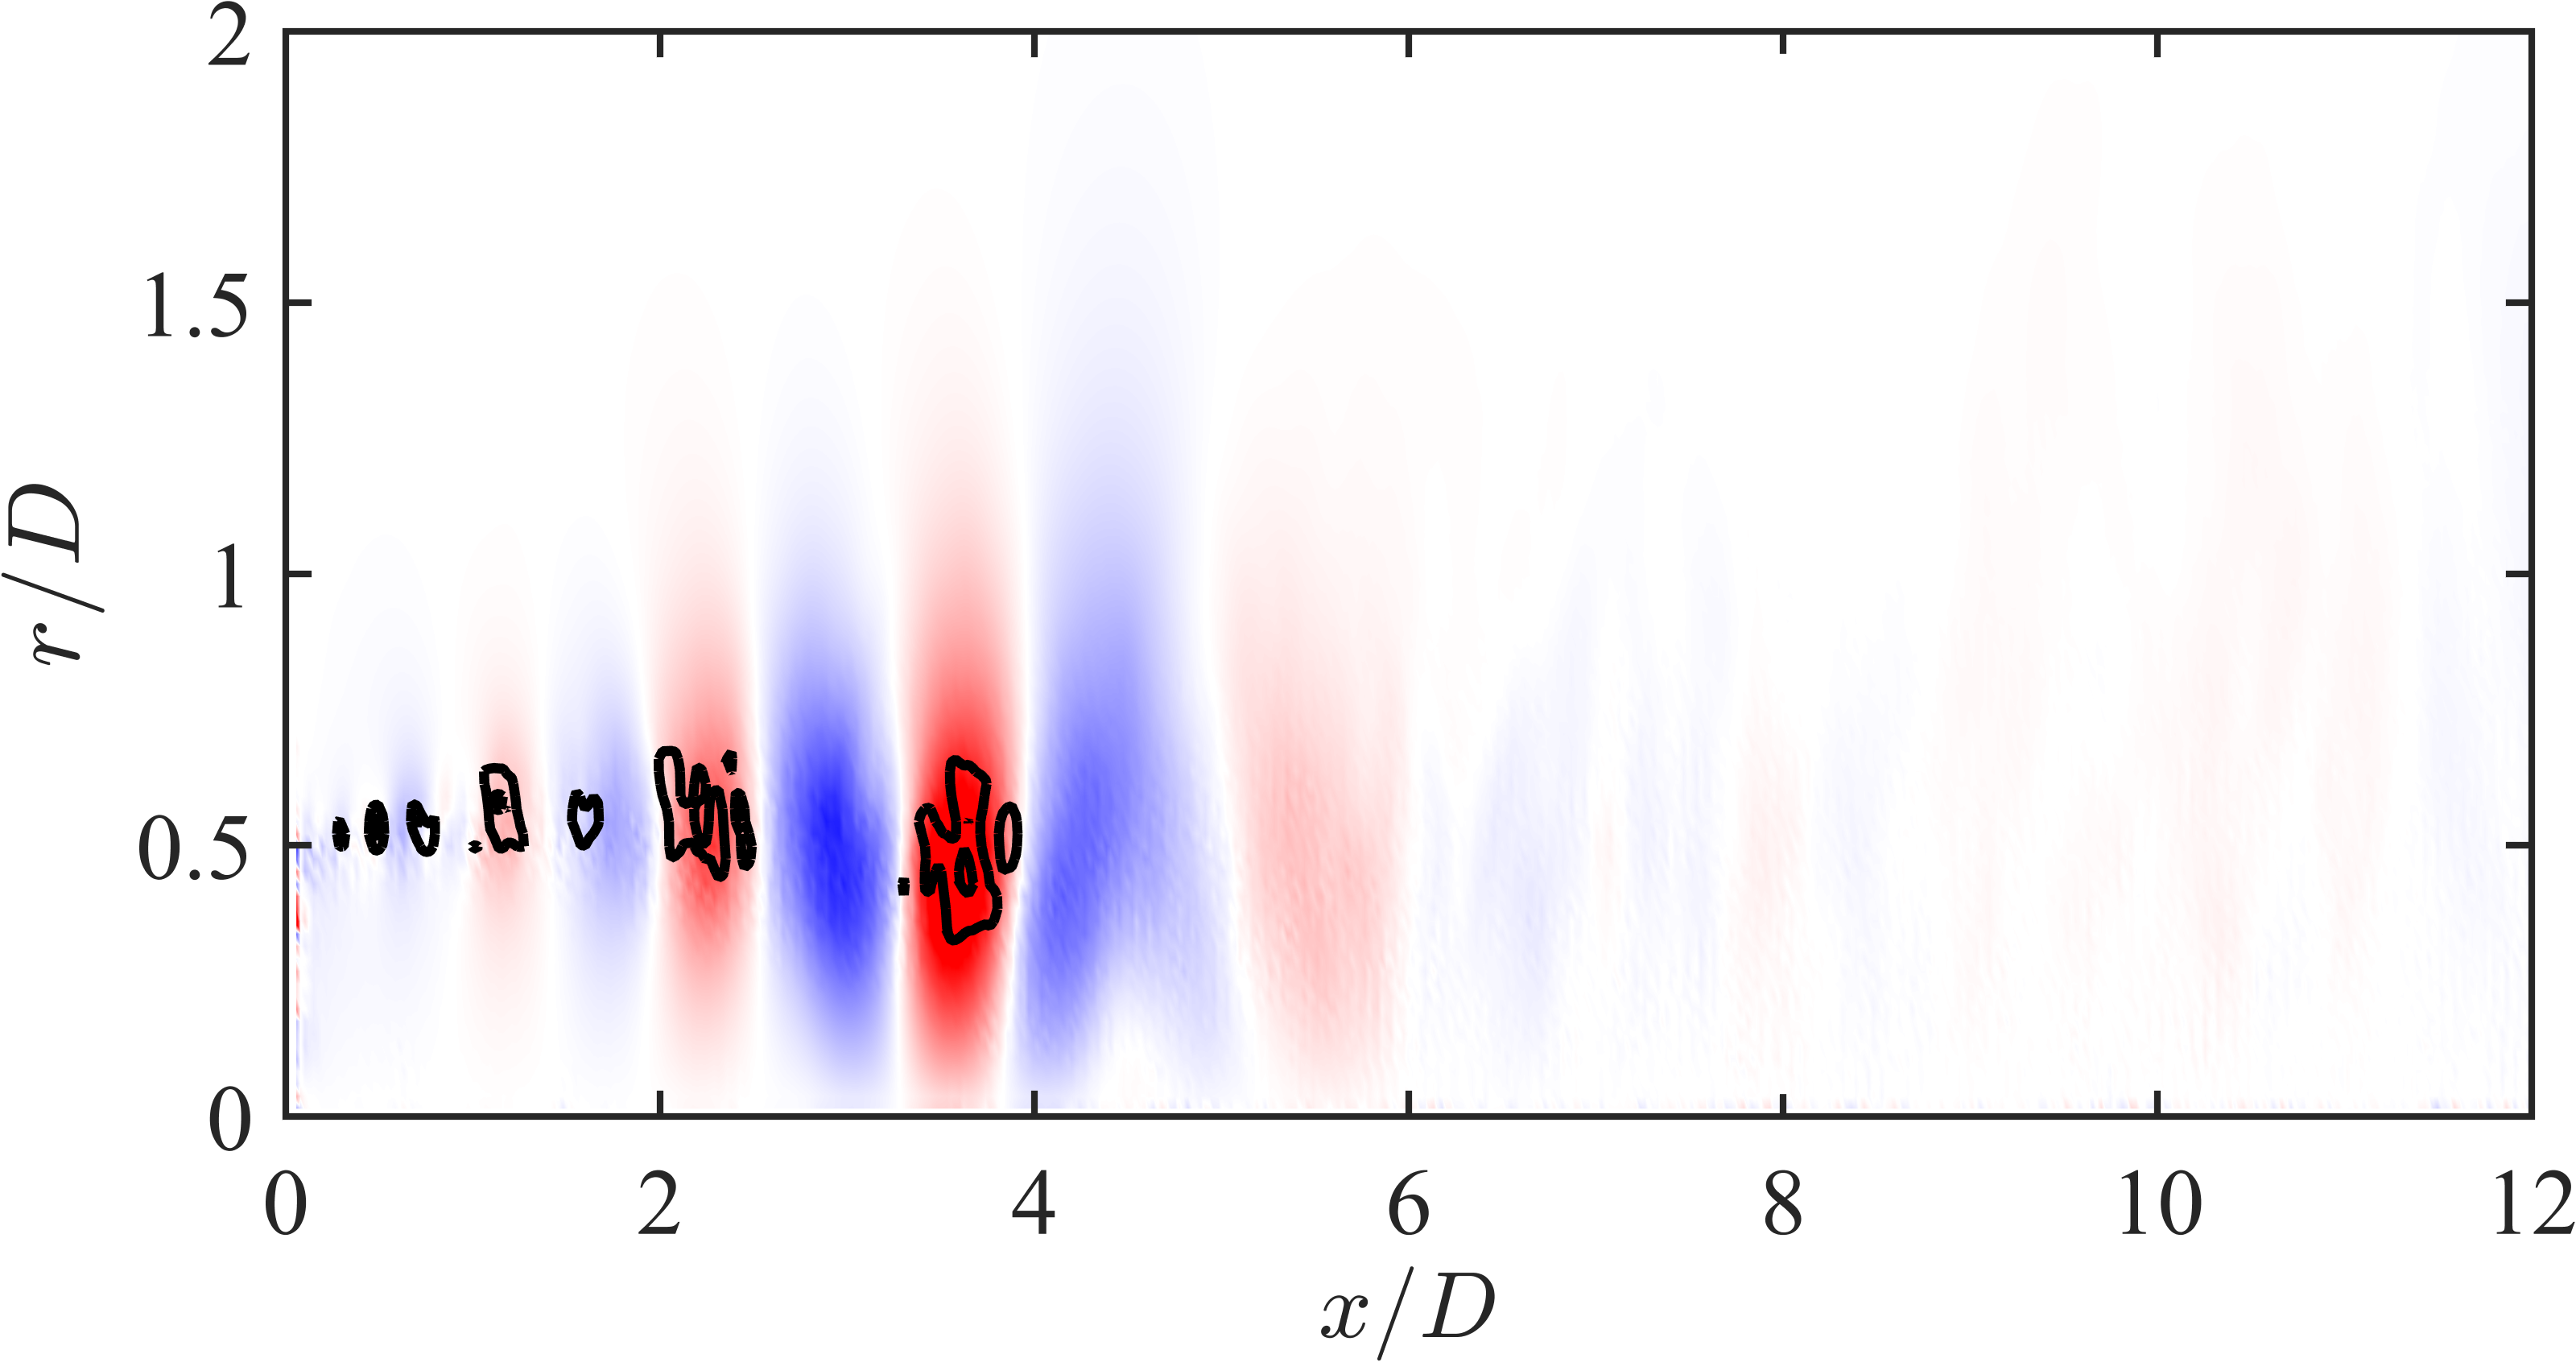
\includegraphics[width=0.95\linewidth]{Figures/ch5_St005_SL_131.png}
%		\caption{$St_{DF} = 0.05$}
%		\label{fig:SL_St005}
%	\end{subfigure}\\
%	\begin{subfigure}{0.75\textwidth}
%		\centering
%		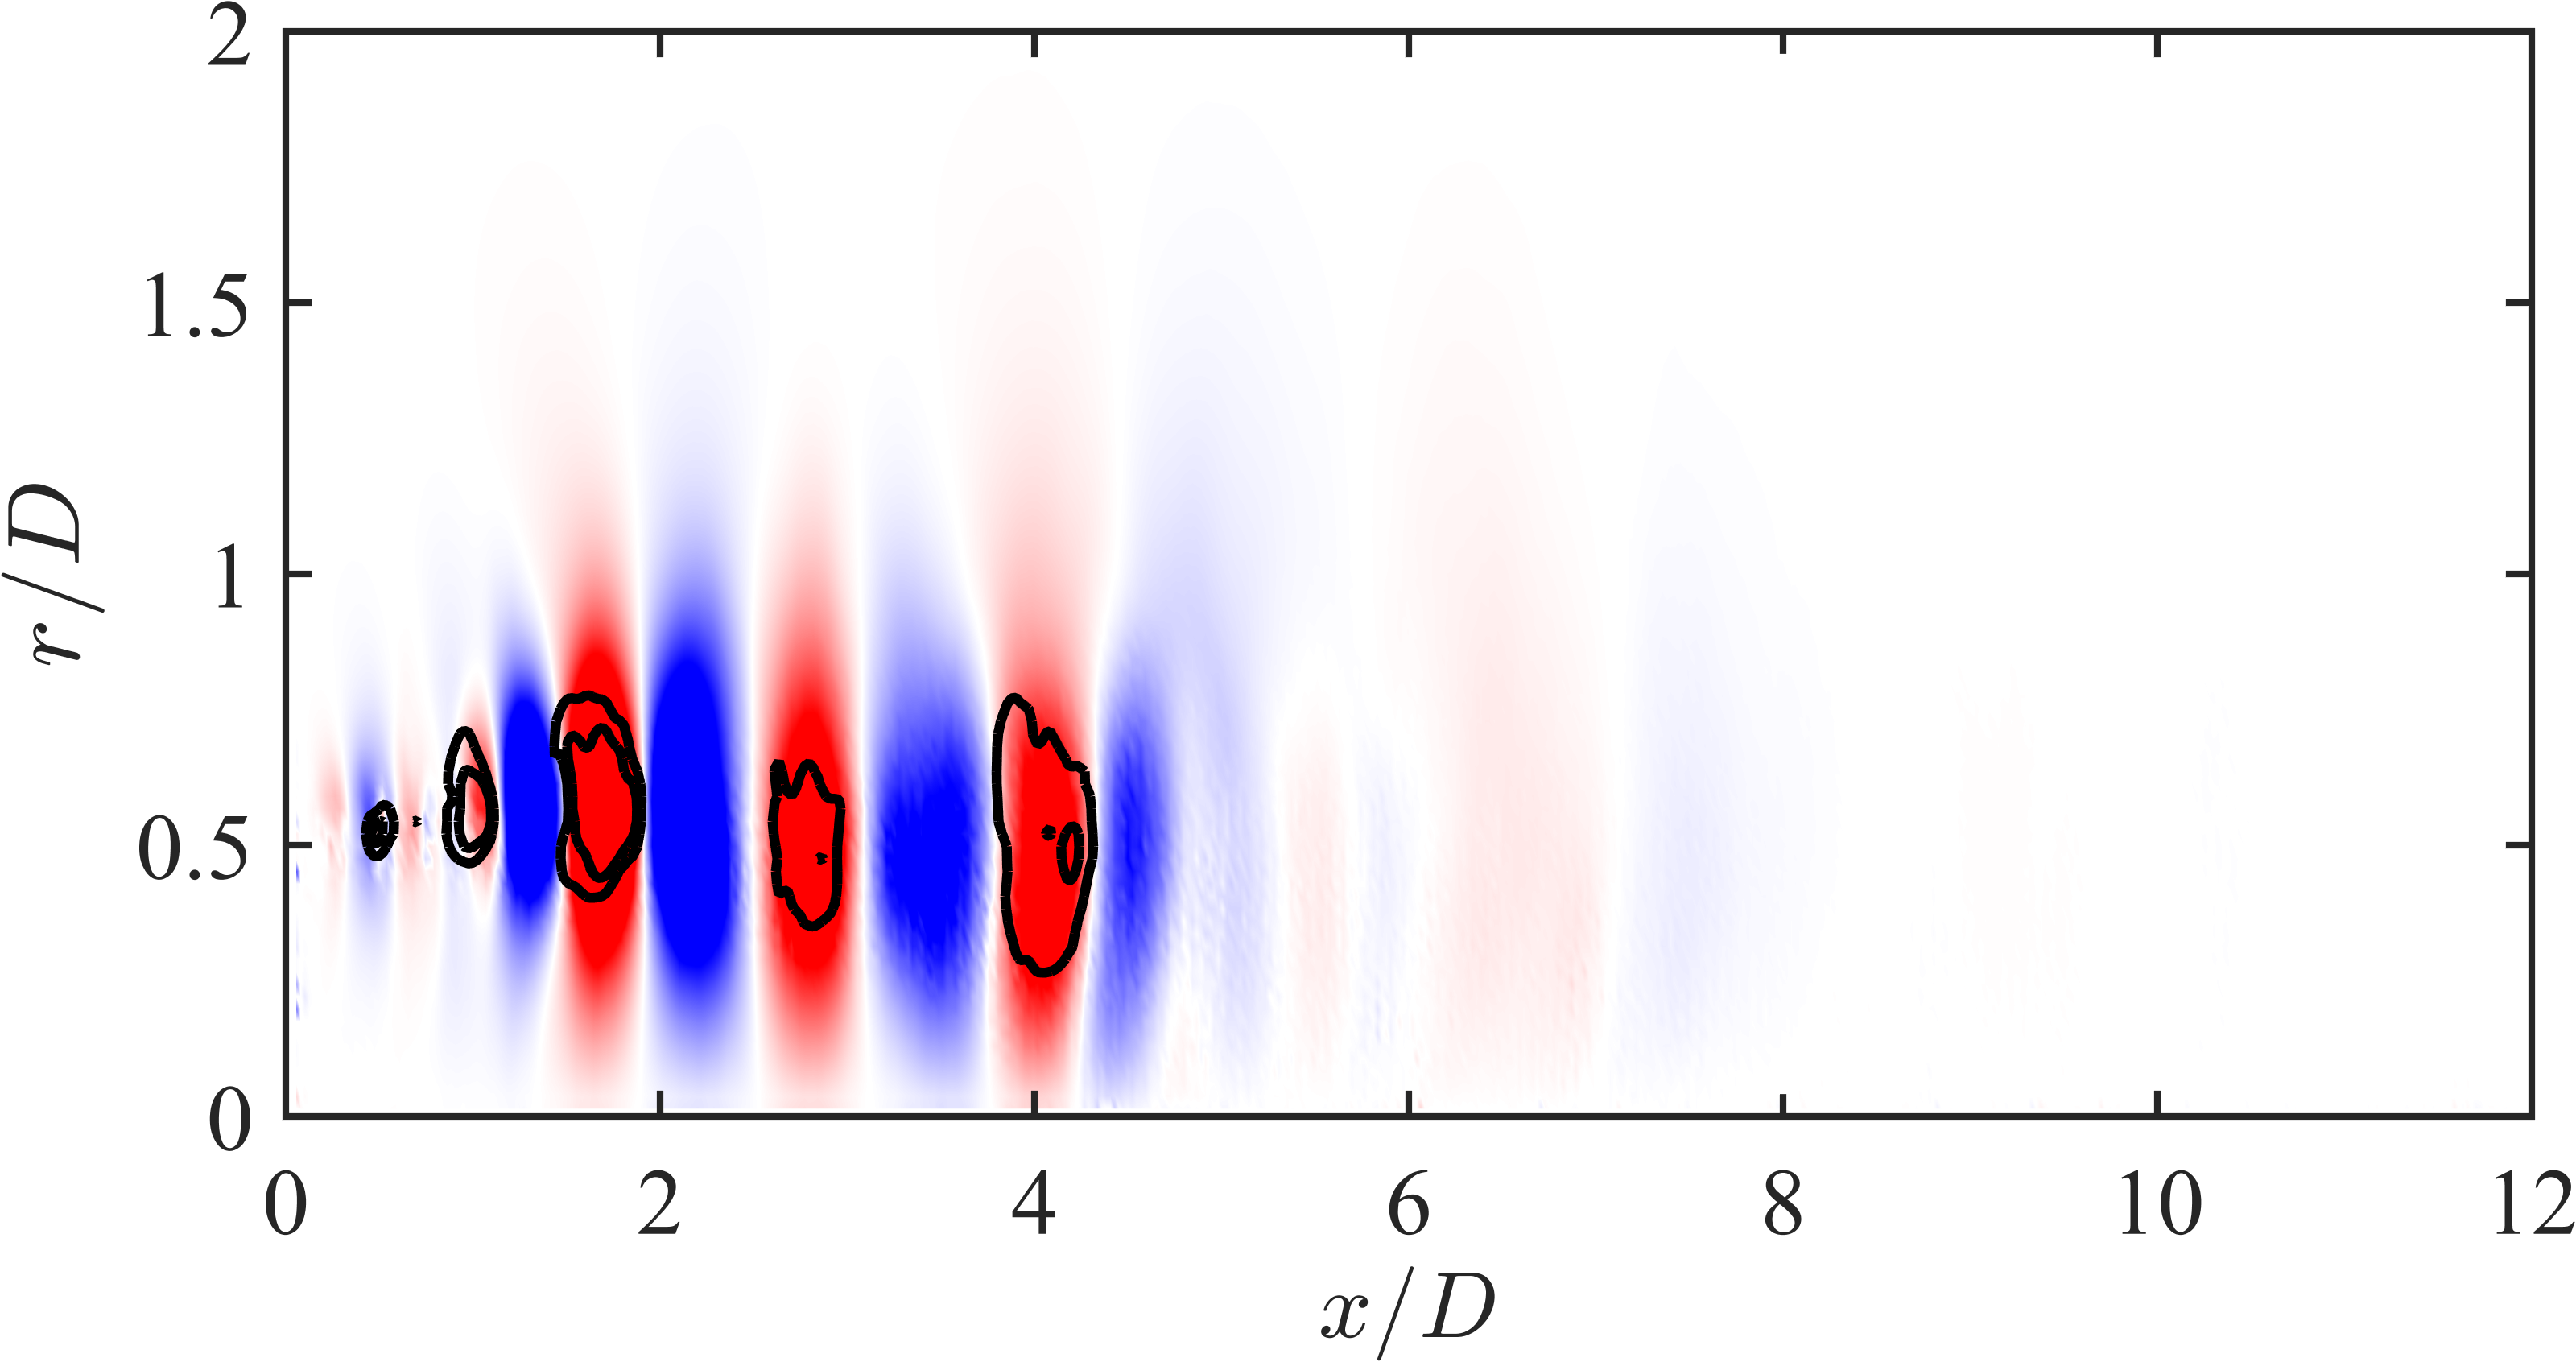
\includegraphics[width=0.95\linewidth]{Figures/ch5_St025_SL_1.png}
%		\caption{$St_{DF} = 0.25$}
%	\end{subfigure}
%	\caption{Aeroacoustic source wavepackets induced by the large-scale structures. For readability, the colormap has been inverted from previous figures; here regions of red indicate positive fluctuations.}
%	\label{fig:SL}
%\end{figure}
%
%This issue was explored in depth by Cavalieri \etal \citep{Cavalieri2010} using analytic models for subsonic wavepackets.
%By allowing the wavepacket amplitude and spatial extent to vary in time (termed `jittering' by the researchers), the superdirective, intermittent acoustic emission pattern observed in high-speed jets was recovered and the predicted amplitude was within 1.5 dB of the measured.
%A similar modulation of the spatial extent and amplitude of the source wavepackets can be observed here, depicted in \fig{fig:jittering}.
%For the impulsively-excited jet, a single dominant acoustic source region is observed, modulated in space and time per the passage of the large-scale structures, and located at $ 2 \lesssim x/D \lesssim 6$.
%As discussed previously, corresponds to the disintegration of the large-scale coherent vortices as they begin to self-interact near the end of the potential core.
%For the $St_{DF} = 0.25$ excitation case, the overall amplitude of the acoustic source field is much higher than for the impulsively-excited case.
%However, a similar modulation of the amplitude and spatial extent is observed here.
%Unlike the impulsively-excited case however, the periodically-excited jet has, in addition to the downstream acoustic source, a high-intensity source region  for $x/D \lesssim 2$, corresponding to the pairing of the multiple harmonic structures generated per excitation pulse.
%That the significant amplification of the fluctuating Reynolds' stress produced by the vortex merging is amplifying the source field, is unsurprising.
%For this excitation frequency, the results of \sect{sect:nearfield} indicate that this is ultimately failing to significantly affect the far-field acoustic emission, at least at low polar angles.
%\begin{figure}
%	\centering
%	\begin{subfigure}{0.33\textwidth}
%		\centering
%		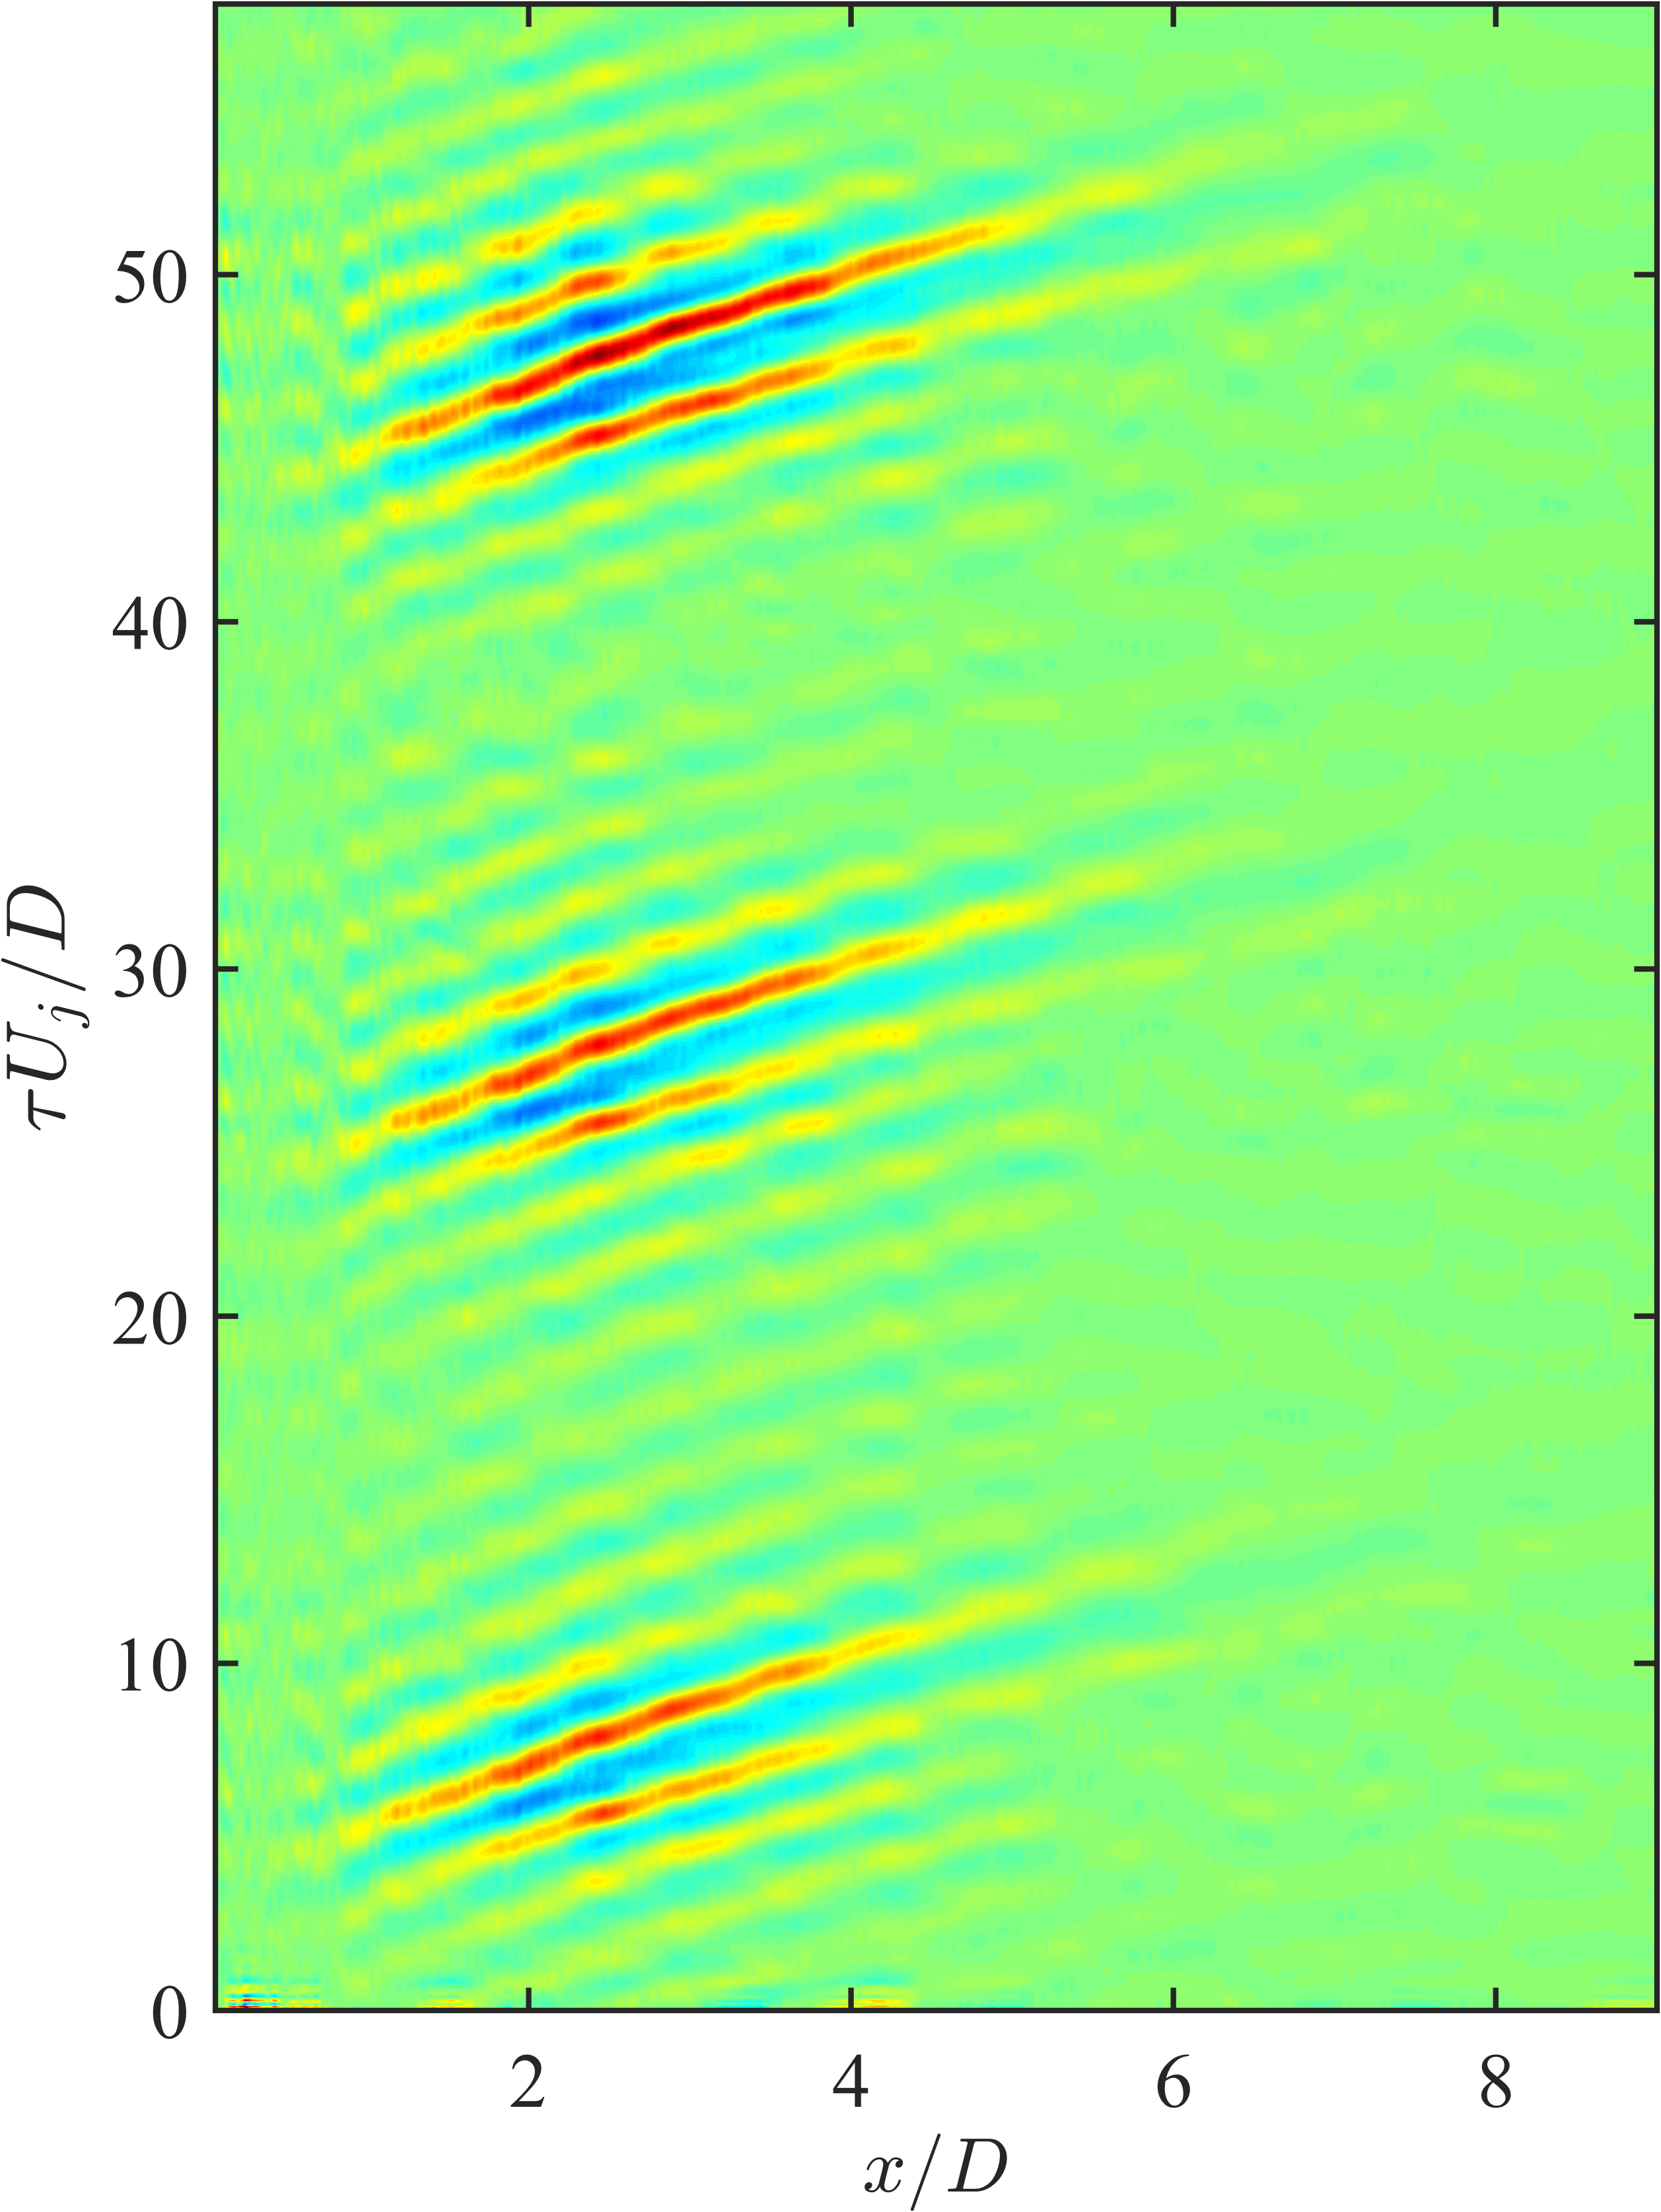
\includegraphics[width=0.95\linewidth]{Figures/ch5_St005_modulated_source.png}
%		\caption{$St_{DF} = 0.05$}
%	\end{subfigure} % %
%	\begin{subfigure}{0.33\textwidth}
%		\centering
%		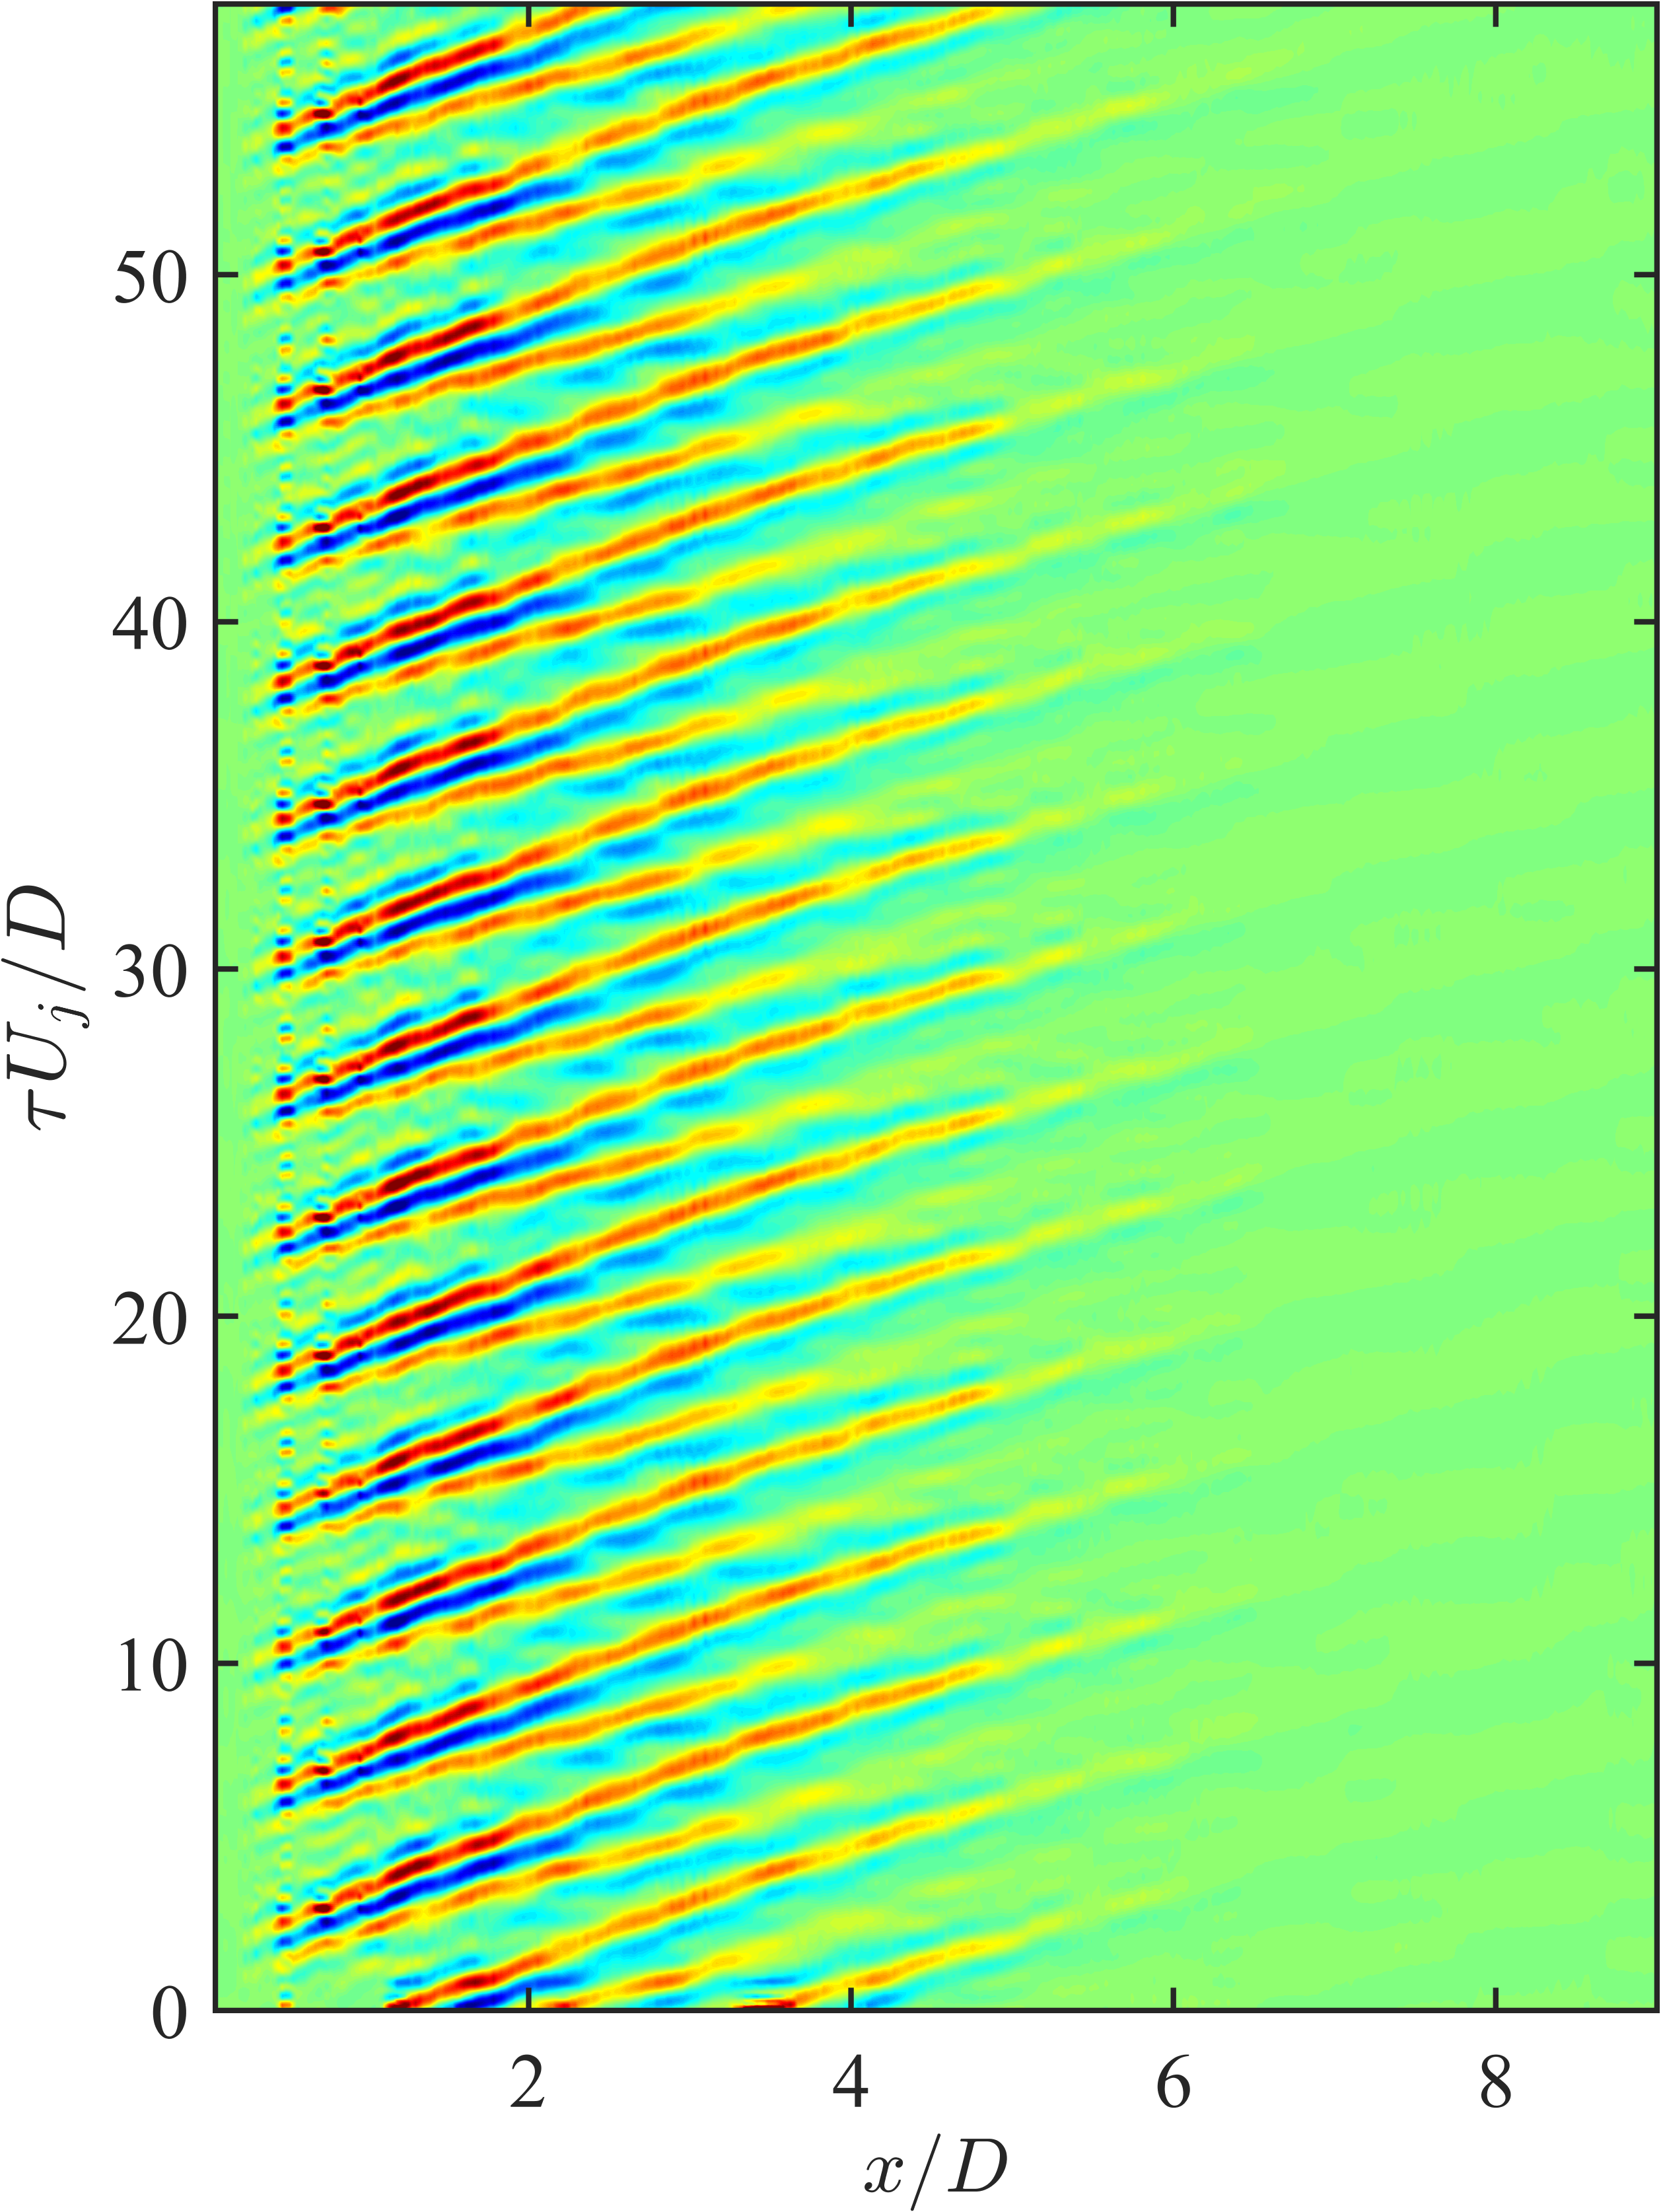
\includegraphics[width=0.95\linewidth]{Figures/ch5_St025_modulated_source.png}
%		\caption{$St_{DF} = 0.25$}
%	\end{subfigure}% %
%	\begin{subfigure}{0.33\textwidth}
%		\centering
%		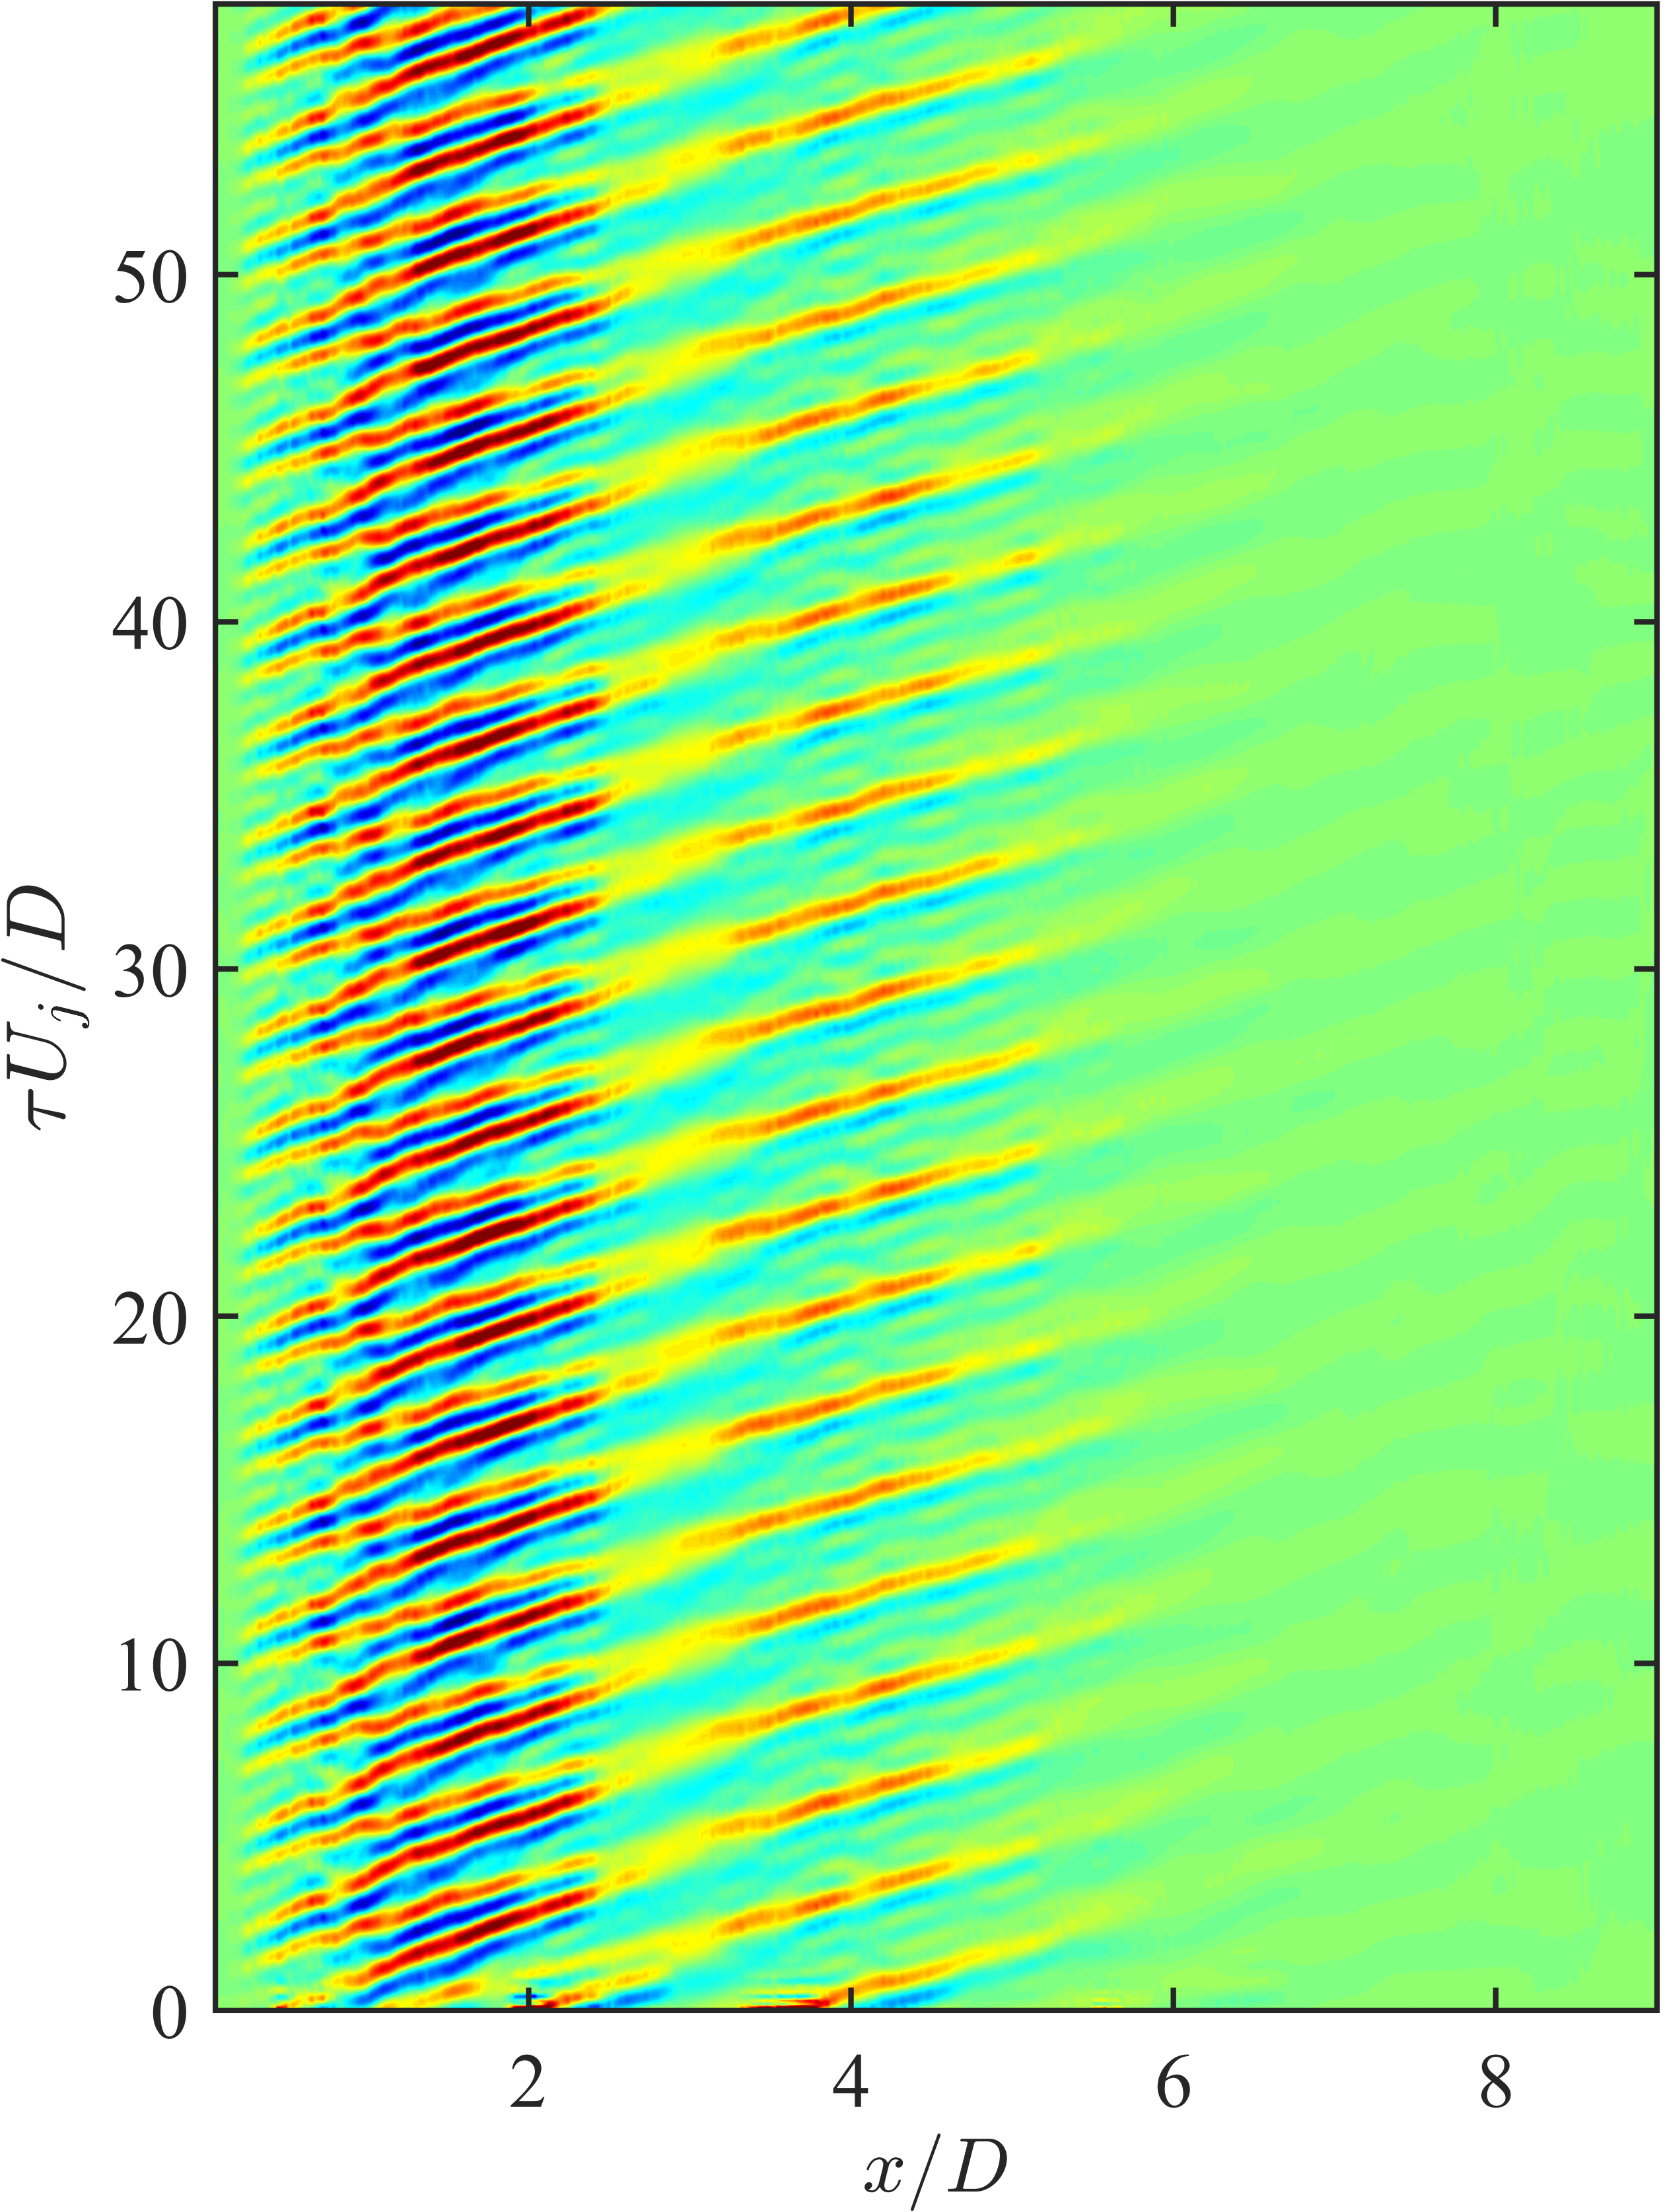
\includegraphics[width=0.95\linewidth]{Figures/ch5_St035_modulated_source.png}
%		\caption{$St_{DF} = 0.35$}
%	\end{subfigure}
%	\caption{Spatio-temporal modulation of the aeroacoustic source as measured along the lipline of the jet.}
%	\label{fig:jittering}
%\end{figure}
%
%As the excitation frequency is further increased to $St_{DF} = 0.35$ however, the relative importance of the aeroacoustic source associated with the vortex merging is significantly increased.
%The source field in the $St_{DF} = 0.35$ exhibits two highly distinctive regions in which the waveform undergoes a rapid modulation; this is in contrast to the results for $St_{DF} = 0.25$, where the source associated with the vortex merging and the source associated with the structure disintegration appear combined.
%Vortex merging has been experimentally identified as acoustically important in low-speed, low-Reynolds number jets \citep{Kibens1980}.
%The results of this section indicate that, under the right circumstances, vortex merging might also play a non-negligible role in the noise generation process in high-speed turbulent jets.